%% thesis.tex
%%
%% this file, mythesis.tex, is the main file of a fictitious
%% Penn State Ph D thesis
%%
%%
%% this material can be used as a template to prepare your own Ph D thesis
%%
%% this file was created Sept 1995 by Stephen G. Simpson,
%% simpson@math.psu.edu
%%
%% revised November 1996, S. Simpson
%% revised 2002, Sarah Gallager (to allow deluxetables)
%% modified a little more by Michele Stark (2004)
%% modified to use the new psuthesis.cls (Mar 2005) with a signature
%%   page and a committee page

\documentclass[11pt]{psuthesis}

% % Please add the following required packages to your document preamble:
% \usepackage[table,xcdraw]{xcolor}
% If you use beamer only pass "xcolor=table" option, i.e. \documentclass[xcolor=table]{beamer}
\usepackage[normalem]{ulem}
\useunder{\uline}{\ul}{}

%% optional packages, in case you want AMS math macros and AMS symbols
\usepackage{amsmath,amssymb}
%% allows bibtex, \citet{}, \citep{} referencing:
\usepackage{natbib}
%% I truthfully don't know what the following is for, but I never used it:
%\citestyle{aa}
%% optional package, in case you want PostScript graphics:
\usepackage{graphicx}
%% the following allows you to use the AAS deluxetable environment:
%\usepackage{deluxetable}
%% Use the following if you have tables that are longer than a single page::
%\usepackage{longtable}
%% Use the following if you have (non-deluxetables, i.e., longtables) that
%% you need to display landscape oriented:
%\usepackage{lscape}


% \usepackage{balance}       % to better equalize the last page
% \usepackage{graphics}      % for EPS, load graphicx instead
% \usepackage[T1]{fontenc}   % for umlauts and other diaeresis
% \usepackage{txfonts}
% \usepackage{mathptmx}
\usepackage[pdflang={en-US},pdftex]{hyperref}
% \usepackage{color}
% \usepackage{booktabs}
% \usepackage{textcomp}

% Some optional stuff you might like/need.
\usepackage{microtype}        % Improved Tracking and Kerning
% \usepackage[all]{hypcap}    % Fixes bug in hyperref caption linking
\usepackage{ccicons}          % Cite your images correctly!
% \usepackage[utf8]{inputenc} % for a UTF8 editor only


%% for a less-than-final version of the thesis, this command
%% places "DRAFT: <date> AT <time>" at the top of each page...
%\thesisdraft
%% (comment this out for the final version)

%% you can speed things up by compiling only one chapter at a time
%\includeonly{somechapter}
%\includeonly{someotherchapter}
%\includeonly{yetanotherchapter}
%\includeonly{Ithinkyougettheideachapter}
%\includeonly{conclusions}
%% (comment this out for the final version)

%% Fix the text citations so that there is no comma between the authors and
%% year.  This will help contain the furious Brandt red pen.
\bibpunct{(}{)}{;}{a}{}{,}

%% Change the fonts back to something reasonable.
%% Note: scriptsize is typically smaller than footnotesize.
%\renewcommand{\scriptsize{\@setfontsize\scriptsize\@ixpt{9pt}}
%\renewcommand{\footnotesize{\@setfontsize\scriptsize\@xpt{10pt}}

%%
%% These are all the definitions that I've used throughout my thesis.
%\input{/enter/path/to/your/definitions}

\begin{document}

%%Comment this out for the final thesis:

%%

%% at the beginning of the thesis we have a title page, a signature
%% page, and an abstract

\author{Dong Chen}


\title{\uppercase {Supporting Collaborative Information Analysis Using interactive Visualization: A Design Research}}

\dept{Information Sciences and Technology}

\submitdate{Dec 2020}

\copyrightyear{2020}


% \begin{singlespace}

\readerone{John M. Carroll \\
         Distinguished \prof{Information Sciences and Technology} \\
         \adviser \\
         \chair}

\readertwo{Alan MacEachren\\
           \prof{Geography} \\
           Affiliate \prof{Information Sciences and Technology} \\           
           Director of GeoVista Center}

\readerthree{Xiaolong Zhang \\
             \assocprof{Information Sciences and Technology}}

\readerfour{Mary Beth Oliver \\
             Donald P. Bellisario \prof{Media Studies} \\
             Co-Director of Media Effects Research Laboratory}


%%   Key to titles:
%% Associate Professor: \asocprof{of what}
%% Assistant Professor: \assistprof{of what}
%% Full Professor: \prof{of what}
%% also Dept. Head: \head{of what}
%% You can also do things like: ``Associate \head{of what}''

\begin{frontmatter}

%this is the ``normal'' signature page from the original version of the class
\signaturepage

\begin{doublespace}
\titlepage
\end{doublespace}

%this is the new committee page
\committeepage

\abstract

Collaborative information analysis is a form of sensemaking that involves modeling and representation of complex information space through synchronous and asynchronous team interactions over extended periods. Effectiveness of collaboration determines team performance, which directly impacts the justice of decisions made or solutions proposed. Effective collaboration is challenging because extra efforts are required to develop and maintain team awareness on top of information analysis task, which itself demands a high need of cognition.

A lot of research has been conducted to support collaboration and information analysis \textit{separately}. For example, numerous tools and techniques have been developed to facilitate the processing and visualization of information analysis, but the majority are designed for individual use rather than for collaborative use. On the other hand, collaborative tools, also known as groupware, are developed to improve team effectiveness, yet they often lack support for advanced information modeling and representation. A gap exists between the two research areas, a design space yet to be explored when a \textit{team} is engaged in collaboratively analyzing a set of data. Simply applying design implications from both areas together should not work because we must address the tension of need for cognition in both the task of collaboration and the task of information analysis. To some extent, the task of collaborative information analysis is a different activity from either. People are engaged in a different workflow and face new challenges, which this research tries to understand and support.

Evaluating effective tool support for collaborative information analysis is another multifaceted and complex problem. Researchers often reduce the complexity of the analytic task for the sake of ease of measurement. In practice, it is challenging to model complex analytic scenarios in lab studies which span only a couple of hours, and real cases and professional analysts are often limited to access in reality. However, the level of task complexity directly determines the need for cognition in analysis and influences the collaboration strategy teams will employ. This research addresses the challenge of empirical evaluation and targets at situations in which professionals need to both analyze complex information and collaborate about decisions.

My research starts with a task analysis of an example of collaborative information analysis in the real world: an undergraduate course of intelligence analysis at Pennsylvania State University. I described student analysts' workflow and their team behavior with current tooling. Specifically, the study observes that structured techniques are frequently employed but lack serious collaborative support. Based on the observation, five design objectives are proposed for a better collaborative tool. These objectives drive the design and development of a new tool out from this dissertation, \textit{CAnalytics}, an integrated analytic workspace that supports real-time collaborative data annotation for information modeling and collaborative data visualization for information analysis. 

\textit{CAnalytics} is evaluated in two classroom studies, in which students are being trained to become professional information analysts. I did a quantitative analysis on system logs and student reports, as well as a qualitative analysis of questionnaires. The first study emphasizes assessment of integrating structured information modeling and visualization in a single collaborative workspace. I analyze different team behaviors on multiple dimension, and their interaction with team performance. The second study focuses on supporting a higher-order information analysis activity, i.e. collaborative hypothesis development, using a structured approach. Both studies contribute to the understanding of analysts' team behavior in collaborative information analysis and the role of computing tools in support of both collaboration and information handling.

In summary, this dissertation contributes an understanding of how analysts use computing tools for collaboratively analyzing information in the real world. The research produces a collaborative visualization tool that leverages structured techniques from the intelligence community as well as design knowledge of team awareness from the CSCW (Computer-Supported Collaborative Work) community. The classroom studies evaluate design choices and help identify emerging design challenges. The dissertation ends with design implications and proposes that structured techniques and collaboration be enablers for each other.





%% this is the end of the abstract

%% after the abstract come the table of contents, the list of tables,
%% and the list of figures
%% Note about the figure list... so the figure list is a decent length,
%% use the following command for the figure captions:
%% \caption[Short figure title to appear in figure list]{Normal figure caption}
%% (this trick unfortunately does not work with the deluxetable
%% ``\tablecaption'' command, so be careful what you put in the table captions)
%%
%% If you have really long tables that cover multiple pages, you
%% will want to use the ``longtable'' environment (it is very similer to
%% deluxetable) but allows you to specify headers and footers for the first,
%% last, and middle pages of the figure.

%% use this command to omit the list of tables,
%% if the thesis doesn't contain any tables
%\nolotables

%% use this command to omit the list of figures,
%% if the thesis doesn't contain any figures
%\nolofigures

\tables

%% next come the acknowlegements (optional) and the preface (optional)

\acknowledgments  % optional

I would like to express my deepest appreciation to  Dr. John M. Carroll, my advisor, for his support and guide during my doctoral program. He brought me into the world of Human-Computer Interaction and has been continuously inspiring me to be innovative and curious of the unknown.

My thanks also go to my committee members, Dr. Alan MacEachren, Dr. Luke (Xiaolong) Zhang, and Dr. Mary Beth Oliver. Their constructive criticism helps improve the quality of this research significantly.

The classroom studies of this research were conducted in the course by Col. Jake Graham and Dr. Luke (Xiaolong) Zhang. I would like to thank them for providing me with such a great research opportunity. This research will not be possible without their support. 

Finally, I want to thank my wife, Bing Wang, and my son, Leo Chen, for their love, patience, and belief in me. 

This material is based upon work supported by the National Science Foundation, under Award No. 1450893, 2014-2015. It was also supported by assistantships at Pennsylvania State University. Any opinions, findings, and conclusions or recommendations
expressed in this publication are those of the author and do not necessarily reflect the views of the awarding agencies.


%\preface    % optional

\clearpage
%
%\vspace*{2.0truein}
%
%\LARGE
%\parbox{4.0truein}{
%\par\noindent
%Rome did not create a great empire by having meetings, they did it by
%killing all who opposed them.\\
%\hspace*{\fill}--Unknown
%}
%\normalsize

\end{frontmatter}

%% this is the end of the front matter

%% now we include the actual chapters of the thesis
%% there are individual chapter files ch-intr.tex, ch-over.tex, ...
%% (NOTE: you do not need the ``.tex'' extention on the file name
%% in the include statement)
%% these chapters can be in a sub-directory, for example:
%% \include{chapterdirectory/chaptername}

\chapter{Introduction}
\section{Introduction}\label{introduction}

\subsection{Motivation}

Collaborative information analysis is a form of sensemaking wherein a team analyzes a complex information space of facts and relationships to identify and evaluate causal hypotheses. It is conducted in various domains and its effectiveness is critical to the justice of the resulting decision and conclusion. A common example is crime investigation \citep{kirk1953crime}; a variety of putative facts are assembled, including financial records, witness observations and interviews, and social connections of various sorts among persons of interest, from which investigators collaboratively assess means, motives, and opportunities, articulate and investigate further hypotheses and deductions, and develop one or more theories of the crime. One of the challenges is the volume of information and the level of sophistication of relationships among the information, which could easily go beyond the capacity of individual human cognition. 

Collaboration is critical in such complex tasks. Effectiveness of collaboration determines team performance, and thus the justice of decisions made or solutions proposed. Researchers have repeatedly found evidence of low performance of distributed groups compared to face-to-face groups (as reviewed in \cite{Olson2000}). They have attributed the performance issues to extra efforts required to maintain \textit{awareness} \citep{Heath2002d, Gutwin1998f} for distributed groups. To collaborate effectively, people need to know a lot about their collaborators: where they are, what they are looking at, what they are working on, what they recently did, what they are planning to do, what they know, what skills they have, who they know that might know something, and so forth. None of the information, however, is intuitively available in distributed settings.

 Indeed, many deficits exist that could result in disruptions in the flow of communication within distributed groups \citep{Carroll2009i}: field of view diminished, facial expressions are limited, the possibility to use gestures is reduced, sharing of tools and artifacts is constrained, and exchanged information could be delayed. Further, in the case of miscommunication, it is difficult to repair, or even discover the resulted misunderstanding. Even worse, the challenges become more salient as the range and complexity of the task expand. 
 
Collaborative information analysis tools, also known as Information analytical groupware \citep{Grudin1994e}, are designed to facilitate analytic collaboration and collaborative sensemaking.
Numerous tools have been developed in the research community. However, these works often focus on amplifying individual cognitive abilities (e.g. \cite{Stasko2008, Bier2008}), or collaboration with relatively simple tasks (for example, trip planning). Most of them lack complex serious empirical evaluation studies \citep{Goyal2016,Convertino2011}, or do not include a full-featured supporting tool \citep{Carroll2013,Borge2012}. The state-of-the-art analytic tools that are currently widely used, such as IBM Analyst's Notebook \citep{IBM}, and PARC ACH \citep{PARC}, are designed for individual use only. 

\subsection{Problem}

This dissertation describes and discusses \textit{a design research that developed and evaluated groupware for supporting collaborative information analysis}. 

A critical challenge for information analysts is building a structured preliminary data model and ensuring that the data model is employed effectively in hypothesis development and evaluation \citep{wongsuphasawat2019goals, kandel2012enterprise}. This is an open challenge. Standard structured techniques often do not support it at all; for example, Analysis of Competing Hypotheses (ACH) assumes that data has been modeled, and that relevant evidence can be adduced appropriately to various hypotheses, but provides no structured support for either \citep{Gelder2008}. My work aims to build an integrated environment which bootstraps a structured approach following which analysts can build data model and develop hypotheses in one place. 

Another challenge is to develop and maintain team awareness while engaging in a cognitively demanding task. The concept of awareness has been a major focus in the field of Computer-Supported Collaborative Work (CSCW) \citep{Steinmacher2013a, Carroll2009i, Heath2002d}. Research has investigated many aspects of awareness, its role, and measurement, but its interaction with information analysis, more specifically, usage of structured techniques is less examined. Support for structured techniques are often designed for individuals, and its employment in collaboration is less researched \citep{Heuer2009}. This study focuses on awareness support in applying structured techniques.

Finally, the study aims to understand computer-supported collaborative work in a close-to-reality environment. Many studies look into the usage of low-fidelity tools and usage in a controlled lab experiment over a short period. It remains unclear whether insights gained from
those low-fidelity tools can be applied to more advanced interactive tools. This is especially true for collaborative tools, because tools and teams often develop into a new system over time, and can behave quite differently as the system develops more awareness \citep{Stahl2006}. While new tools bring about new affordances, they inevitably introduce extra constraints. The new affordances and constraints of the tool shape the way users approach a task, and even completely transform the
task itself \citep{Carroll1989}. This research examines how analysts employ high-fidelity groupware in their collaboration and observes their behavior in a natural environment, in particular, in a classroom setting.

\subsection{Research methods}

To address the problem, I started with a task analysis \citep{schraagen2000cognitive} of collaborative information analysis by observing team behaviors in an intelligence analysis course at Pennsylvania State University. Based on the design requirements, I developed a fully functional tool, CAnalytics, which supports collaborative information modeling and analysis. The tool is then evaluated in two intelligence analysis classroom studies. Each study is analyzed with qualitative and quantitative research methods. Results and design implications are reported at the end of each  study.

\subsection{Dissertation structure}

Chapter 2 models the task of information analysis, and explores popular structured techniques. It then turns to a review of research on awareness in collaboration. The chapter ends with a survey of available tools for supporting collaborative information analysis. 

Chapter 3 introduces CAnalytics, a collaborative visualization tool I designed and developed for information analysis. I started with a task analysis and defined five design objectives of CAnalytics. The chapter then highlights the major features of the system and critical implementation details. 

Chapters 4 and 5 present two classroom studies that investigate the design and evaluation of CAnalytics. Study One focuses on evaluating the design of an integrated collaborative workspace and the way the structured technique is performed. Study Two examines collaborative hypothesis development. Each study yields design implications for the field.

Finally, Chapter 6 reflects on the research method and lessons learned from the result. 


\chapter{Literature Review}
\section{Task of Collaborative Information Analysis}

Collaborative information analysis is a form of sensemaking wherein a team
analyzes a complex information space, assertions involving people, places,
transactions, and events with varying relevance to the analysts’ concerns from
sources with varying credibility and reliability. In general,
analysts seek to identify relationships beyond facts that are literally specified in the original data. Taking a broad view of the task, collaborative information analysis happens in lots of group activities that are data intensive. Different forms of collaborative information analysis tasks
are actively explored in various research domains. For example, collaborative
information seeking (CIS) \citep{Shah2014i} is capturing increasing attention as
complementary to traditional individual information seeking. Beyond simply
searching and collecting information, researchers note that CIS requires
participants to also analyze and understand information \citep{Paul2010}, which is similar to what we address here. Also, the visualization
community investigates interactive visualization techniques to assist collaborative
analysis, known as collaborative visual analytics \citep{Isenberg2011}, in which a team relies on the
``use of computer-supported, interactive, visual representations of data with
the common goal of contributing to joint information processing activities''
(p. 312). Further, Web 2.0 techniques make ``social data
analysis'' possible, wherein any people can upload and share a dataset, and gain
collective insights \citep{Morton2014}.

Other examples of collaborative information analysis include
intelligence analysis where professional analysts integrate evidence and
expertise to support hypotheses \citep{Heuer1999}, scientific collaboration in
which researchers piece together established theories and new findings to
explain a phenomenon \citep{Farooq2009}, crisis management
where stakeholders share crisis context and resource distribution to make rescue
plans \citep{Tomaszewski2012b, Convertino2011}, healthcare services where doctors share
a patient’s information and make diagnostic decision \citep{Reddy2008c}, daily
trip plan where a family synthesizes information about tourist resorts and plans
the route, and many other scenes. 

To address the challenge of cognitive load and collaboration, we
target those information analysis tasks with complex data nature. Specifically, we investigate in the domain of Intelligence Analysis. 

\subsection{Modeling the task of information analysis}
Given the similarity of information analysis in different domains, researchers have proposed conceptual models to characterize the practice. These models abstract user behavior patterns and help researchers think of these tasks on a high level, thus guiding the design of supporting tools. Pirolli and Card’s \citep{Pirolli2005}
Think Loop Model (Figure~\ref{fig:pirolli}) is a well-cited model characterizing information
analysis activities. The model describes the iterative process of information
foraging and sensemaking in which raw evidence is successively aggregated,
filtered, and synthesized into the most reasonable hypothesis. In the model, analysts first
identify and collate relevant information from external data sources. From this
collection, they then organize an evidence file of propositions that can be used
to make inferences. They next integrate evidence into problem-oriented schemata.
These schemata are used to articulate hypotheses, which are evaluated to
determine the best story of the information. The model is a bottom-up process of
structure building, but also includes a local feedback loop at each stage. Thus,
analysts can reconsider propositions in the evidence file, asking how they are
related, or a given hypothesis, asking what schemata it rests upon. While the
Think Loop Model identifies various leverage points for information analytic
tools (especially in the area of visual analytics), Pirolli and Card acknowledged that the
model was only a starting point to investigate the domain. Many problems remain
unanswered by the model. For example, the model is targeted at individual
information analysis and does not account for the social process in
collaborative information analysis: How do analysts share their evidence files?
How do analysts synthesize their information schema? How do analysts negotiate
their hypotheses? Besides, the model stands from a data-centric view, describing
how data transforms and flows, rather than the way analysts work and transition
\citep{Kang2012b}. The work processes, however, are important to
develop a useful and usable system that can be integrated in real practice and
ultimately transform the current practice.

\begin{figure}
	\centering
	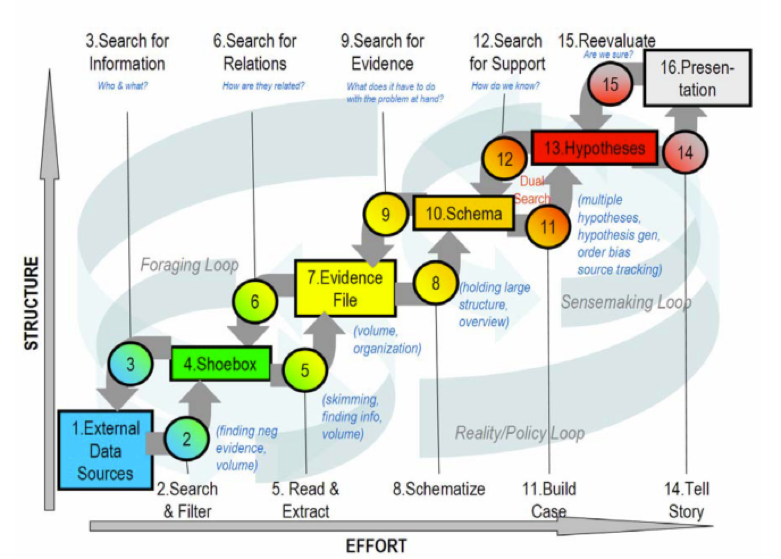
\includegraphics[width=.8\columnwidth]{02-Literature/img/pirolli.png}
	\caption{Pirolli and Card's Think Loop Model)\label{fig:pirolli}}
\end{figure}

While Pirolli and Card's model suggests a more linear-like model, Wheaton \citep{Wheaton2011} addressed a 
parallel, or multi-phased model. He conceptualized the process as four functions: conceptual modeling, data collection, data analysis, and report production. The four functions are not in sequence, but all begin almost immediately. Throughout the course of the analysis, the dominating function could shift at some point, and the amount of time spent on each function could change. Similar patterns were observed in Borge et al.'s study \citep{Borge2012}. They observed behaviors of reading, sharing, synthesizing, interpreting, decision making, and receiving new information, yet no linear pattern or order of flow from one behavior to the other is observed. The workflow seems very flexible. Similar reports were conducted in Herrmann et al's study \citep{Herrmann2013a}.

\begin{figure}
	\centering
	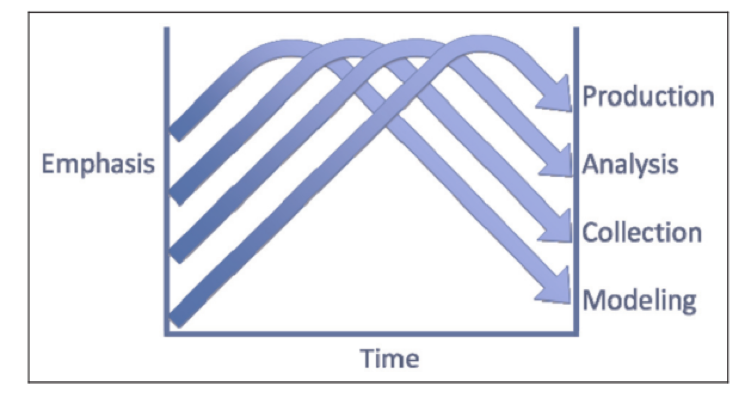
\includegraphics[width=\columnwidth]{02-Literature/img/wheaton.png}
	\caption{Wheaton's multiphasic model of information analysis process)\label{fig:wheaton}}
\end{figure}

Several empirical studies are conducted to contribute to a deeper understanding
of the process of collaborative information analysis. For example, \cite{Chin2009} observed practices of five professional intelligence analysts. Their report serves as an important source of truth because most professional analysts are inaccessible due to the classification level of
the content they address. They reported analysts first made annotations in their
source materials to highlight purported facts about people, places, and events,
then they constructed various artifacts to hold and present facts, and finally,
they tried to identify patterns or connections among facts. 

\cite{Kang2012b} chose intelligence analysts in training as the research target at a compromise of difficulty of accessing intelligence analysis professionals. They conducted a longitudinal observational field study of analysts' training course. They summarized that the analysis process covered four phases
overall: conceptual model construction, information collection, information
analysis, and production. Their observation highlighted a number of
misconceptions designers might have about the intelligence analysis. For
instance, intelligence analysis was more of an exploratory activity than an
answer-finding process. Analysts might not have a specific hypothesis in mind;
instead, they were like ``cutting a path through the jungle that’s never been
explored'' \citep[p.145]{Kang2012b}, and did not necessarily know where they
were going. Also, analysts did not rely
on a specific analytic tool; they tried out various techniques and strategies to
solve a problem. 

Another type of empirical study is a laboratory
experiment, in which ordinary people are usually recruited to perform a
controlled task, either with a low-fidelity prototype (e.g. paper and pen) or
existing commercial analytic tools. The premise is that observations of people’s
interactions with non-digital artifacts can help reveal the basic work processes
and thus inform functions digital tools should support. People’s interactions
with familiar tools would reflect the way they understand and think about the
problem at hand. For instance, \cite{Borge2012,Carroll2013} developed a crime investigation scenario and recruited
college students to investigate into the case as groups. They identified six
primary activities: 1) reading/searching intelligence reports, 2) sharing
information, 3) synthesizing information, 4) interpreting information, 5) making
final decisions, and 6) receiving new information. With paper and pen,
participants spontaneously created graphic artifacts to aid reasoning and
memory. Most frequently seen artifacts included tables, lists, calendars, maps,
node-link graphs, and text annotations. When comparing performance across
groups, researchers found that in better-performed teams, participants had a
higher proportion of push acts, in which people voluntarily shared information
with partners with being asked to. Also, groups tended to perform better when
they created artifacts to synthesize and schematize findings, in addition to
simply recording facts. Besides, high-performance teams were usually not dominated
by an individual. Collaborators contributed their expertise without block and
shifted authority as needed. Similarly, \cite{Isenberg2008b} conducted a paper-based experiment and observed participants’
temporal sequence of processes in analysis. They derived a framework
characterizing the analysis activities, which consists of browse, parse, discuss
collaboration style, establish task strategy, clarify, select, operate, and
validate. Specifically, they noted that as opposed to many models, no typical
temporal ordering of the sequence was evident. Analysts approach the problem
with different strategies and workflows depending on the problem and the group
dynamics. Findings from these laboratory experiments also contribute to the
understanding of group behavior in information analysis and inform the design of
future systems. 


\subsection{Structured techniques}

Structured techniques are often adopted in information analysis. Compared to casual analysis, which often relies on experience and intuition, structured analysis provides a systematic, transparent method to approach the analytic process. The rationale behind structured techniques is effectively encapsulated by Heuer's claim \cite[p.31]{Heuer1999}: 

\begin{quote}
	Intelligence analysts should be self-conscious about their reasoning process. They should think about how they make judgments and reach conclusions, not just about the judgments and conclusions themselves.
\end{quote}

Structured techniques externalize internal thought in a systematic and transparent manner so that they can be shared, extended, and critiqued by other analysts. Thus understanding structured techniques and their application in the state-of-the-art is critical in designing and supporting collaborative information analysis. 

However, due to the complexity of these techniques and limited support of technology, the practice of structured techniques is often simplified or even abandoned \citep{Chin2009, Wright2006}. It is an open question to address the tension between the benefit of structured technique and time cost in implementation. In this section, we review three structured techniques that have been widely used in the intelligence community and their challenges.

\paragraph{Analysis of competing hypotheses}
Analysis of competing hypotheses (ACH) \citep{Heuer1999} emphasizes a rational, transparent process of analysis. The general steps of ACH are designed for systematic assessment of all hypotheses and evidence. These steps include identifying a complete set of hypotheses, identifying all pieces of evidence, assessing the diagnostic value of each evidence against each hypothesis, and drawing conclusions of the likelihood of hypotheses. The principle of ACH is to refute rather than confirm alternatives. ACH guarantees an appropriate analytic process and increases the chance to avoid common analytical pitfalls. Studies by \cite{Lehner2008} and \cite{Lord1979} demonstrate the function of ACH in reducing confirmation bias, the tendency to seek and interpret evidence in favor of a theory perceived most likely a priori. PARC ACH \citep{PARC} is an implementation of ACH, facilitating hypothesis and evidence input and assessment. 

Yet ACH has several pitfalls. For example, ACH does not provide a measure of uncertainty among hypotheses. Efforts have been made to combine ACH with probability reasoning systems, such as pairing with Bayesian Network \citep{Karvetski2013} or Bayesian statistical model \citep{Duncan2008}. Our project differs from these efforts in that we employ a human-center approach and investigate how technology could assist teams of human analysts in applying structured techniques effectively.

Gelder \cite{Gelder2008} listed five problems of ACH from a practitioner’s experience. For example, ACH treats evidence as an individual entity, forcing analysts to assess the value on its own with each hypothesis. In practice, however, evidence diagnosticity is often mediated by other propositions; judgment of one item of evidence is based on the judgment of several other items. The rigid matrix structure of ACH does not allow for the factoring of these mediating propositions. Also, the ACH matrix represents hypotheses in a “flat” structure: each hypothesis is entered individually across the top row. In many cases, a more flexible representation of hypotheses is needed. For example, a general hypothesis can have sub-hypotheses, and two seemingly distinct hypotheses at the beginning of analysis might evolve into another alternative in a later stage. Such a hierarchical structure of hypotheses is unlikely to be represented in ACH. Besides, the judgment of the consistency of evidence with each hypothesis is decontextualized. Analysts have to make a judgment on whether each item of evidence is consistent or inconsistent with hypotheses, but the supporting evidence for that judgment is not represented or documented anywhere. The issue, known as data provenance, is critical in information analysis \citep{Chin2009}. Lack of data provenance makes it difficult to ground a judgment, resolve group decision conflict, or correct mistakes. 

In addition, we observed several deficiencies of ACH in our observation of student analysts performing ACH in class when we worked with instructors in the Security and Risk Analysis program. For example, manual efforts are required in generating and updating views of data. Analysts have to manually copy and paste evidence from a document into cells of ACH matrix. This is not only a redundant effort but also subject to errors in the process. This also results in a missing connection between evidence in the matrix and the source of evidence in the original document. It is difficult to review the credibility or reliability of a piece of evidence later. Besides, information analysis is a dynamic process: analysts tend to re-interpret and re-assess evidence iteratively. Once evidence is changed, analysts have to manually change the evidence in the ACH matrix as well, which again increases the chance of error.

Besides, ACH demands a high expertise bar for analysts. Users are required to identify a complete set of mutually exclusive hypotheses at the very beginning, which is difficult for people with little expertise and experience in the domain. Further, hypotheses tend to evolve as analysis proceeds. A hypothesis valid in the beginning may no longer be of value later, or two seemingly separate hypotheses in an early stage of analysis could be combined in a way to better explain the situation later on. The assumption ACH makes that all hypotheses and evidence are identified and set in the very beginning limits the dynamic development of analysis. 

We propose to address these problems by employing a more flexible approach and leveraging several other structured techniques. Our tool integrates information gathering with information analysis so that analysts can develop hypotheses based on their generated data models and the insights can be traced back to the context where data models were created. Building on the data models, we leverage such structured techniques as link analysis and evidence marshaling to assist analysts in hypothesis discovery and development. 
 

\paragraph{Link analysis}
Much of the data in intelligence analysis can be represented in link form, as a collection of connected nodes.  Examples include contact reports (two people witnessed together at a specific time and place), phone calls, and financial transactions. Link analysis enables analysts to see the bigger picture of connections, and also reveal patterns that might otherwise remain unnoticed. Link analysis helps analysts answer questions such as “who is central in this organization?”, “What role does an individual appear to be playing in an event?”, “How is this event related to other events?”, etc.
 
Link analysis is a popular structured technique employed in the intelligence community. In their empirical study of professional intelligence analysts, \cite{Chin2009} emphasized the importance of link analysis in the reasoning process. They observed that analysts created graphs by hand drawing facts and relationships, or used Microsoft PowePoint to construct the network. A number of specialized tools are available, including i2 Analyst’s Notebook \citep{IBM}.  These tools provide node-link visualizations and facilitate storing, modifying, organizing, and querying links. But these tools are designed for individual use only. For collaboration, participants have to either be physically co-located and share the same screen, or screen capture the visualization and manually share it through other tools. 

Another issue of link analysis tools, similar to PARC ACH, is that analysts have to duplicate data from the document space to the analytic space; they have to manually construct entities and relationships in a separate tool, which, again, is not only time-consuming but also might introduce unnecessary errors and lose data provenance. 

Moreover, a criminal network is often characterized as dynamic rather than static \citep{Sparrow1991}. The relationships between entities often have a temporal distribution. For example, a person who is trivial in an organization might become critical later, or in a specific event period. This dynamic network feature often fails to be reflected in link analysis tools due to their lack of temporal data structure. 

Our tool employs multiple coordinated views. We display temporal data in a timeline, spatial data in a map view, and relationship data in a node-link graph. Views are coordinated, meaning that change in any one view will cause a change in another view. Thus analysts can investigate the criminal network during a specific time range when applying a temporal filter on the timeline, or network within a specific geographic area when applying a spatial filter on the map. 

\paragraph{Evidence marshaling}
Evidence marshaling is a common technique to tie the evidence to hypotheses and assertions. The technique connects bits of information together and provides a big picture of the story. It is an important step in Pirolli and Card’s sensemaking model \citep{Pirolli2005}. Without tool support, analysts often do a simple, informal marshaling in their minds. With an elaborate computer-based method, analysts can coordinate events along a timeline, or organize evidence into stories about typical topics (e.g. what, when, where, who, and how).  

Several tools are designed to support evidence marshaling. For example, Entity Workspace \citep{Bier2010} displays an entity-based view of documents. Users can organize their entity-based evidence into collapsible stories. Jigsaw \citep{Gorg2014} implemented a ShoeBox tool for evidence marshaling and note-taking. Users can record hypotheses and connect them with supporting or contradicting evidence. However, they eventually abandoned the design because it ``was just too complex and did not allow analysts to take free-style notes in the way they would do on paper'' \citep[p. 342]{Gorg2014}. As an alternative, they designed Tablet, a simplified tool for evidence marshaling, which essentially is a networking tool linking entities as well as the interpretation of entities. An advantage of the Tablet is that it becomes more flexible and users can do a free-style note-taking much like on paper. Another recent tool is SAVANT \citep{Goyal2016}, in which participants could make sticky notes anywhere in the dashboard, and connect notes as their sensemaking process proceeds. They also include a hypothesis window, allowing users to explicitly enter their hypotheses and supporting or refuting evidence. Similar to the result of Jigsaw, however, their user study indicates that the interface is too complex and discourages users from using it. Sandbox \citep{Wright2006} takes the metaphor of paper and analysts can arrange information within the workspace to their need. Rich interactions are designed to facilitate information manipulation. A limited user study was conducted, however, to prove its effectiveness in supporting analytic process.


\section{Collaboration and Awareness}

While several attempts, as discussed above, have been made to implement support for various structured techniques, most of them are designed for individual use only. However, prior work \citep{Chin2009, Warner2008} emphasized that the work of information analysis at non-trivial scales is fundamentally collaborative, and that the single person operating the software is a bottleneck to the team process. A report from National Intelligence \citep{Vision2015} states that intelligence analysis increasingly becomes a collaborative enterprise, with the focus shifting “from traditional emphasis on self-reliance toward more collaborative operations ”. This is a major change from the traditional concept of intelligence analysis as largely an individual activity.

Structured techniques are reported to be best utilized in a group effort so that collaborative opinions insights could be built \citep{Heuer1999}. The transparency of structured techniques ensures that divergent or conflicting perspectives among analysts are heard and seriously considered early in the analytic process. For example, ACH is often used in team collaboration because ACH leaves an audit trail showing what hypotheses were identified, what evidence was used, and how they were interpreted. If teammates disagree, the ACH matrix could highlight the source of disagreement, and be used to ground further team discussion. Te@mACH is a recent advance in ACH technology, developed by Globalitica, LLC, in 2010. It is designed as a collaborative version of PARC ACH. It allows distributed analysts to work on the same ACH matrix simultaneously. Other tools for supporting structured techniques, however, mostly remain a single-user application. 


With single-user applications, teams of analysts have to rely on external view sharing tools \citep{Greenberg1990} or manually share notebooks and screenshot graphs. This has the consequence that the tools are employed only at specific points in an analysis, often only in the early stages during which analysts are working on their own. Indeed, the use of these tools directly diminishes a team’s activity awareness, requiring repeated manual resynchronizing to identify redundant or missing pieces of information, analyzes of information, and analytic hypotheses. This can be mitigated through maintaining and pooling individual analysis reports using Google’s real-time editing tool set, Google Doc, Google Sheets, Google Calendar, etc. These tools enable collaborative document editing, and provide a revision history list of changes made to a document by each collaborator, supporting awareness of teammates’ contributions. However, the Google tools themselves are not integrated; each tool manages its own data representation. Thus an event report in Google Doc cannot be exported to Google Calendar or Google Map. Non-existent or weak support for coordinating multiple visual representations could undermine activity awareness. We found this to be a specific source of problems in our study of spontaneously created physical visualizations in the information analysis task \citep{Carroll2013}.

Vision 2015 also notes a shift “away from coordination of draft products toward regular discussion of data and hypotheses early in the research phase”. This emphasizes the importance of close coupling collaboration in the analytic process, as opposed to simple coordination as the final step. A key enabler of such effective and close collaboration is activity awareness, a critical concept for research in computer-supported collaborative work (CSCW). In prior work Carroll and his team \citep{Carroll2003, Carroll2011j} developed a conceptual framework, conducted design research investigations of software tools \cite{Carroll2003,Carroll2009i,Ganoe2003}, carried out field studies \citep{Ganoe2003,schafer2008emergency}, and made controlled experimental studies \citep{Convertino2008,Convertino2009,Convertino2011}. That body of work produced several results: Activity awareness can be measured, though this entails methods beyond those traditionally employed in awareness research, including conversation analysis \citep{sacks1995lectures} and artifact analysis \citep{fleming1974artifact,pearce1994thinking}. Activity awareness grows with the development of reciprocal knowledge about, experience with, and trust of partners. It is facilitated when the sharing of collaborator-specific knowledge is implemented as an explicit, public and documented interaction within the collaborative activity; indeed, activity awareness can be increased beyond measured levels in face-to-face interactions \citep{Convertino2011}, a rare result in computer-supported cooperative work (CSCW) sometimes referred to as “beyond being there” \citep{hollan1992beyond}. The growth of activity awareness qualitatively changes coordination strategies that partners adopt (for example, early in a collaboration, members pull information from partners by voicing their needs and concerns to the team, but subsequently, as team members become more aware of the responsibilities and roles of other members, they selectively push information to fellow members). Thus, becoming a team does not merely speed up or improve coordination; it changes what coordination means and what members do to coordinate. Activity awareness engages active and meta-cognitive strategies for improving team cognition, for example, through negotiating and sharing ad hoc representational artifacts \citep{Carroll2013}. Finally, activity awareness can be effectively supported with interactive tools, and the benefits of supporting it can be measured. 

More nuanced team behavior is reported in empirical studies. For example, \cite{Chin2009}'s study observed that the analysts  preferred to review the original source material.  Analysts had distinctive and strong beliefs about the artifacts they created themselves, yet claimed they would not trust another analyst’s artifacts, although they believed they could achieve better results by collaborating with others. In another study, \cite{Kang2012b} found that analysts worked as a team throughout the process and the degree of collaboration differs depending on the type of task. These findings reveal details of team behavior and are useful in understanding and designing for better collaboration features.



\section{Technology to Support Collaborative Information Analysis}

A number of tools have been developed to support information analysis. For example, the Analyst’s Notebook \citep{IBM} and ACH \citep{PARC} are widely used in intelligence analysis areas. However, these tools were developed for individual use only. Prior work demonstrated that the work of information analysis at non-trivial scales is fundamentally collaborative. In practice analysts have to manually share notebooks or graphs to coordinate their work.

As the need of support for collaborative information analysis is capturing increasing attention, more technologies are being developed. Most of the tools take advantage of visualization techniques and display awareness information in a visual way. This is not hard to understand since the human visual channel has a high bandwidth and can take in a large amount of information in a short time. Visualization can efficiently capture user attention and represent awareness information in a concise and vivid way. Fussell and her colleagues \citep{Balakrishnan2010e,Goyal2013,Goyal2016} have done a series of controlled, comparative laboratory experiments investigating the effect of visualization on collaboration. They found that groups using visualization tools had better performance and shared visualization increased group discussion. Various visualization techniques have been designed to facilitate different facets of awareness, and most of them fall into the categories below. 

- Who are collaborators. Knowledge of the existence of potential collaborators and their skills and expertise is important. \cite{Forsen2009a} proposed the concept of Pinpoint, an interactive visualization radially presenting colleagues that are most closely related and affords browsing, filtering, and further exploration of the networks of the organization. \cite{Marlow2015a} examined the effect of visualization on the attitude towards peer collaborators. They found that different details of visualization of work history have a different impact on behaviors and attitudes towards collaborators, which further influence group engagement.
  
- What are they doing. While it is easy to know what collaborators are doing in face-to-face settings, e.g. pointing at a figure, walking towards a whiteboard, etc., such signals are nonexistent in distributed collaboration and have to be explicitly supported by technology. Therefore \cite{stefik1987wysiwis} introduced WYSIWIS (What You See Is What I See), in which collaborators share the same view. While this design ensures everyone looks at the same thing, it blocks production as only one person has control of the view at one turn. A relaxed-WYSIWIS design \citep{Gutwin1998h} was then proposed, which enables team members to have control of their own view while having a miniature overview of partner’s workspace, known as radar view \citep{Gutwin1996}. Radar view conveys information not only about what collaborators are doing, but also where they are working on. Greenberg et al. (1996) also proposed the idea of telepointer, where participants can see the mouse cursor of their colleagues. They then further augmented telepointers with traces be means of visualization of the previous motion of the remote cursor. This provides a bit of context of the cursor and makes the mouse gestures easier to interpret. Similarly, \cite{Hajizadeh2013} attempted to support awareness of collaborator’s activities by visualizing their bushing actions. They found that persistent selection, which adds a “fading-away” effect to past selections, gets people more aware of collaborators’ activities. Technologies as such are often applied in synchronous collaboration, attempting to help collaborators stay aware of what others are doing by embodying a remote gesture in visualization.

- What have they done. People may not be active in a team for all the time. When they come back it is important to know what collaborators have done and what changes they have made. In their approach to visualizing the change of data, \cite{Schumann2013a} used color to encode when a node was created. They also provided a replay function to show the evolution. Similarly, \cite{Edwards1997i} visualized the history as a non-linear tree and argued that the design enabled transition from loosely-coupled work to tightly-coupled collaboration. In the context of collaborative Web search, \cite{Paul2010} posited that displaying users’ search history avoids duplicated efforts and increases team performance. 

- Information sharing. Making sure everyone in the group has access to all information and is aware of the existence of the information is essential for collaborative information analysis. Participants can implicitly share information. For example, \cite{Goyal2014} examined the consequence when user-generated notes are automatically shared with other teammates. They found that participants remembered more clues about the task and participants perceived the tool more useful when implicit sharing is available. However, users may not want to share everything. They also need more control over what to share and what to keep private \citep{Mahyar2013b}. \cite{Convertino2011} designed an explicit but low-cost sharing mechanism through a “Copy-To” button. Analysts could create geo features on their private map and only share those features they wanted to onto a public map by manually clicking on the button. The function grants users explicit control over their acts but requires extra efforts. \cite{Nobarany2012} attempted to combine the advantages of explicit and implicit sharing. They introduced the concept of “obscurity of privacy” and posited that information in a public space can still maintain some level of privacy, depending on the availability of the information to others, awareness of the availability, and the amount of attention it receives. In their system, users can mark a piece of information as private, public, or published. Private information is only kept to the user who produced it. Public information is visible to all group members but does not show up on a highlighted position. Published pieces are not only visible to the group but also highlighted. The effect of this more sophisticated sharing mechanism, however, required further research, according to the authors. 

- Insight sharing. Sharing insights enables people to build on the endeavors of teammates and get aware of what others are thinking or why they are doing that. In the project of Many Eyes \citep{Viegas2007}, a social visual analytic platform where people can collectively analyze data and share visualizations, the primary way to exchange ideas is through the comment system, where users can see other people’s comment on a specific state of visualization. Another social platform, sense.us \citep{Heer2008a}, supports doubly-linked discussion, which means that comments and visualizations are bi-linked: a comment is attached with a visualization (same as Many Eyes), and a specific visualization is linked to comments if anyone has already commented on that state. 

Annotation is a widely used technology to externalize analysts’ insights. For example, \cite{Xiao2008c} asked participants to annotate the rationale when they are performing an act, and found these annotations help other people understand why their colleagues did that. \cite{Hopfer2007b} designed a geospatial annotation mechanism, which attached annotation to a specific area of the visualization. This provides the annotation with clearer context. \cite{Dorn2015a} went further and constrained an annotation with a temporal dimension. Their system allowed students to annotate on a specific position of a video at a specific time point. The system helped instructors know better about students’ puzzles and problems. 

However, tools supporting information analysis are often targeted at a single phase of activity, and thus not supporting the whole workflow. For example, research efforts have been made to understand information collection and modeling \citep{Shah2014i, Jansen2010c}, but little support is provided to extend these models to analysis. Techniques such as Information Extraction and Weight (IEW) helps structures data evidence but offers no structure to turn the evidence to hypothesis development. Similarly, tools supporting the activity of data analysis assume data has been modeled. For example,  Analysis of Competing Hypotheses (ACH) assumes that data has
been modeled, and that relevant evidence can be adduced appropriately to various
hypotheses, but provides no structured support for either. Analytic tools such as interactive visualization emphasize presenting data in insightful means but provides no utility to data re-modeling.
\cite{Ware2012} warned of the \emph{``asymmetry in data rates''} (p.382),
pointing out that visual analytic tools emphasized data flowing from systems to
users far more than from users to systems. Functionalities are mostly designed
to adjust data representation rather than modeling, which are in fact equally
important. Similar calls were made in other data intensive task domains as well. For
example, in interactive machine learning, researchers \citep{Chen2016,Amershi2015} call for an all-in-one environment in which machine learning
practitioners can iteratively refine training data and evaluate model performance through
visualization in one place. Our work aligns with these efforts, and contribute to the design and
evaluation of an integrated workspace in supporting information analysis tasks.

Another gap in the research of collaborative analytic technology is the lack of rigorous empirical evaluations. Little is known how analysts in the real world will employ these technologies in their work processes, and how their work processes will be transformed by these technologies. This study tries to investigate effects of technologies on different facets of activity awareness, and to examine the group processes that make the effects happen.

\chapter{CAnalytics: Tool Supporting \\ Collaborative Information Analysis}
\section{Task Analysis}

We investigated the design needs for collaborative information analysis in three ways. First, we examined existing works that already conducted empirical user studies of information analysts, particularly the works by \citep{Chin2009,Carroll2013,Pirolli2005, Kang2012,Kang2012d}. These works summarize the design needs for supporting collaboration and analytics, as well as empirical user data in support of their arguments. Among them, we used the works by Carroll and his colleagues \citep{Carroll2013,Borge2012,Borge2014} as the most important guidelines because their paper prototype study context was most close to our study. In their study, they observed 22 teams investigating a crime scenario using paper and pen. Teams of participants spent four hours analyzing 222 propositions embedded in a set of problem documents. This study sheds light on team process patterns, collaboration breakdowns, and possible technical support teams need. We reused their experiment materials in our second user study.

We worked closely with the Red Cell Analytics Lab at Pennsylvania State University for over one year. The lab is an instructor-directed student club that is designed to give students experience in analyzing real-world problems to prepare students for the professional world by helping them develop structured analysis skills and critical thinking capabilities. We worked with a fresh student analyst who had just begun to learn the skills and two senior analysts who had more than two years of experience. We met about once every two weeks, observing what and how they performed analytics and having informal interviews in terms of why and pain points.  We also talked to the lab director, Colonel Jake Graham, who had rich in-person experience in professional intelligence analysis before retirement and now a professor teaching analytic skills at Pennsylvania State University. 

We also observed an intelligence analysis course instructed by Colonel Jake Graham. The course  In the course, students learned theories of analysis (e.g. bottom-up analysis vs. top-down analysis, and concepts of hypothesis, assumption, and evidence), analytic techniques (e.g. Analysis of Competing Hypotheses (ACH) \citep{Heuer1999} and Link Analysis \citep{Sparrow1991}), as well as the state-of-the-art tools to support the implementation of those techniques (e.g. PARC ACH \citep{PARC} and Analyst’s Notebook \citep{IBM}. Below we summarized our findings.

\subsection{Major activities: data annotation, data analysis, and hypothesis development}

On a high level, we observed three categories of activities: data modeling, data analysis, and hypothesis generation. A typical workflow is shown in Figure~\ref{fig:workflow}. Analysts received a collection of documents periodically. The documents included police reports, social media collections, news reports, video summaries, and other textual data. Analysts must extract useful information from these documents, connect these pieces of information, make hypotheses of event indicators and warnings. 

\begin{figure}
	\centering
	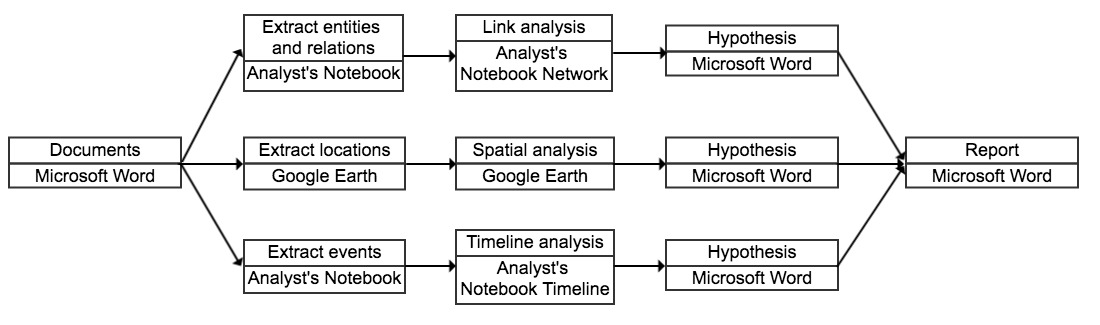
\includegraphics[width=\columnwidth]{./03-System/img/workflow2.jpg}
	\caption{Participant reported intelligence analysis workflow\label{fig:workflow}}
\end{figure}

Upon receiving the documents, analysts would read through and mark critical information. When with pen and paper, they highlighted text and made annotations. They would extract these items and organize them in an ``Information Extraction and Weighting'' table (\ref{tbl:iew_table}). In the table, they investigated each item's face value and alternative value against analytic problems. When with computer support, they created ``entities'' in i2 Analyst's Notebook, a popular software product by IBM for data analysis and investigation. These entities were data objects that described critical attributes and properties. Analysts connected these entities by marking relationships between them. Some frequently seen relationships included ownership, organizational belonging, and phone contact. Location was a special type of entity. To represent the spatial information, analysts replicated the location entities in Google Earth. One interesting detail was that analysts manually exported the location icons used in Analyst's Notebook and imported them into Google Earth. The purpose was to keep consistent the representations in different tools. 

\begin{table}
	\caption{Sample Information Extraction and Weighting table}
	\label{tbl:iew_table}
	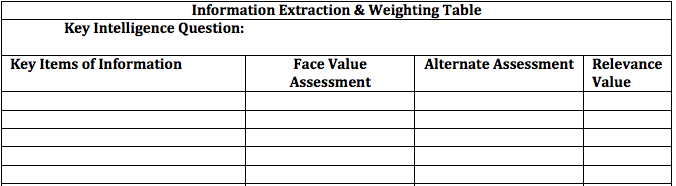
\includegraphics[width=\columnwidth]{./03-System/img/IEW_table.png}
\end{table}

Another special entity type was ``event'', which included a temporal attribute. Event time was important for sequence analysis. Analysts added the start time and the end time of an event, and the repeated date and time if it was a recurring event. 

With the modeled data, analysts tried to find connections and patterns through data visualization. They made use of Analyst's Notebook network tool to map out the entities and their relationships. The timeline tool in Analyst's Notebook displayed the sequential relationship and overlaps between events. They also used Google Earth and identified spatial relationships among events.  To share and keep record of supporting views, they took screenshots and saved in a Microsoft Word document as evidence files. 

Based on these evidence files, analysts generated and recorded hypotheses. These hypotheses are in form of text, but often refer to supporting evidence, either an entity or a visualization of relationships between entities. To compare hypotheses, they often employed the technique of Analysis of Competing Hypotheses (ACH). ACH lays out a full set of hypotheses and examines each item of evidence of its diagnostic value against each hypothesis. Analysts sought evidence to refute hypotheses and picked the least unlikely one. The final delivery was an intelligence report, in which analysts composed their hypothesis and all supporting evidence.

Note that we describe the three activities in a linear fashion for the sake of writing, but analysis could be performed in any order, and most commonly, in an iterative approach.

One problem in the workflow is a breakdown between activities. Systems that support intelligence analysis are aimed at a single activity and therefore only support part of the overall analysis workflow. This imposes a clear boundary between each of these activities on the analysts. For example, IEW helps structure evidence modeling, but does not extend the utilization of evidence to hypothesis generation; ACH assumes that data has been modeled, and that relevant evidence can be adduced appropriately to various hypotheses, but provides no structured support for either. The unintended boundary between phases has the consequence that data modeled in one software cannot be effectively utilized in hypothesis development in another system. And analysts have to handoff, often via replicating the data in the new system, information between software systems, making it difficult to revisit and revise the data model.


\subsection{Collaboration}

Intelligence analysis is fundamentally a collaborative activity because the task can easily become complicated enough that no single individual could handle it. Collaborative intelligence analysis then becomes not only a mental process, but also a group process that involves the management of team resources (tooling, teammate expertise, etc.), teammate goals and motivations, and partner's contemporary and past activities.

Most tools supporting intelligence analysis, however, are not designed for collaborative use. We observed several pain points in participants’ collaboration. For example, participants were unable to contribute simultaneously. Working on the same file would cause conflict. Collaborators had to wait when one teammate was working on the tool. This was known as production blocking \citep{Diehl1987a}, in which individual performing a task became a bottleneck of the team process. To work around the issue, participants often divided their work by tools: each person picked a tool and then created and analyzed an artifact with the tool on their own. This had the consequence that findings and hypotheses be made without integrating collective efforts and diverse knowledge. Participants shared their findings only after they already had a conclusion, which was obviously opposed to collaboration.

Analysts coordinated work outside the tool, by manually sharing documents or graphs through email or cloud storage service (e.g.~Dropbox). As shown in Figure~\ref{fig:workflow}, analysts manually took screenshots of views and copied them into Microsoft Word. This has the consequence that multiple views exist in distributed locations, adding a burden to the analyst’s limited cognition. Analysts could easily overlook certain aspect when they were evaluating hypotheses. The interactive views become static images, making it impossible for collaborators to further explore. Worse, if the data model changes, analysts must manually update the views, resulting in multiple versions of views.
\section{Design Objectives}\label{design-objectives}

Based on our task analysis, we come up with five design objectives for our collaborative analytic tool.

\subsection{Objective 1. Provide an integrated, dynamic  analytic workspace}

While functions can be provided to support a single analytic activity (i.e. data annotation alone, or data visualization alone, and indeed a lot of tools exist to support either activity separately), a critical design objective is to integrate these functions in a single workspace. This is more than simply put together these functions; rather, a smooth transition should be enabled between activities. The goal should be achieved in at least two aspects: (1)
the same data pool and structure is utilized in all analytic activities. Data
created in data annotation can be visualized in analysis, and utilized in
hypothesis development; (2) The system provides a consistent user experience in
different activities. Analysts should be confronted with a consistent user
interface and interaction throughout the process.


\subsection{Objective 2. Support structured data annotating and visualization techniques}

Our design should allow for a structured approach to modeling and analyzing data. Analysts spend a large amount of time and effort annotating critical information from text documents. The essence of an annotation is to turn a set of unstructured, noisy data into structured, useful information while preserving its source. We want to provide a computational method that facilitates the annotation process so that analysts can focus on information itself rather than the logistics. 

The annotated data objects should then allow for a structured analysis of patterns from multiple aspects through visualization. For example, temporal visualization helps analysts keep track of the temporal evolution
of events. Spatial visualization helps identify patterns in the same area. Interactions should be provided so that analysts can coordinate and arrange these views into a bigger picture. These closely presented views form into a proximity-based projection \citep{Kang2014a}, where each view presents a related insight. Analysts can easily navigate these evidence views and marshal them together to support hypothesis development \citep{Pirolli2005}. 

\subsection{Objective 3. Support information sharing and team awareness}

Collaboration is a process of management of team resources and group process. And a pre-requirement for group management is to stay aware of them. We propose to enable real-time data sharing and explicit awareness support.
Analysts should be able to share source documents, annotated data objects, patterned
views, and hypotheses and insights in real-time. Partners can verify who
identified and shared the information and can validate against the source
document to confirm sanity. One’s activities should be transparent to teammates
without extra effort so that everyone is aware of other’s activities.

\subsection{Objective 4. Enabling collaborative hypotheses development}

A more advanced objective is to enable hypothesis development and particularly collaborative development on a team basis. While simply
sharing each teammate's hypotheses is beneficial, its positive impact is
limited to an extent as it is not completely leveraging the various expertise
of a team. Where instead, the combining and evolving of hypotheses from and by
multiple members of the team (where the evidence that the hypothesis is based
on is included in the hypothesis object) creates an environment where the team
is more than just a sum of its parts. We will help analysts to share their
insights/hypotheses with supporting visualization early in the process. To
impart knowledge, visualizations conveniently improve the understanding of
complex problems. When users are exploring the visualization and find
insight, they will be able to share the insight together with the grounding
visualization. The visualization will be interactive rather than a static
screenshot, keeping the ad hoc visualization state. Insofar as stating unknowns
is a difficult task, at least making what analysts do know more explicit and
the assumptions that they made increases a large amount of transparency into
their analysis

\subsection{Objective 5. Capture team behavior}

Other than assisting analysts in accomplishing the task more efficiently, we develop the tool as an instrument to gain a deeper understanding of team behavior. The computing tool can capture and log all interactions analysts have made. These interaction data provide a promising window into which researchers can identify insights in analysis patterns on both an individual level and a team level. Compared to video recording, computing logs have user interaction data already in structure and ready for data analysis without the hassle of human annotating. Log analysis is also easier to scale up to analysis of longer-term interactions than video analysis (e.g. in Study One, we have 73 persons (25 teams),  each person working for about 6 hours, adding up to 428 hours!)

\section{CAnalytics Features}\label{canalytics-features}

\begin{figure}
\centering
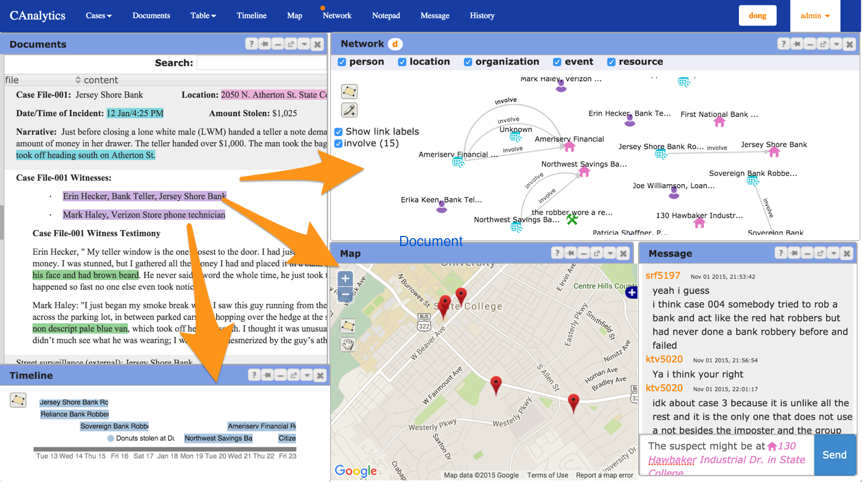
\includegraphics[width=\columnwidth]{03-System/img/interface.png}
\caption{CAnalytics user interface \label{fig:interface}}
\end{figure}

CAnalytics is a web application that aims to provide an integrated workspace
environment wherein teams of analysts identify, visualize, integrate, and assess
facts from multiple sources. The interface is shown in Figure~\ref{fig:interface}. The design is
informed by our cognitive task analysis described beforehand. The system evolved over time. We tagged it as two versions, corresponding to the two classroom studies I have done. Most of the features are available in both v1 and v2, unless noted separately. in v2 we added a couple of new features focusing on hypothesis development, which we will discuss below. 

A use case of applying CAnalytics to an intelligence analysis project: \url{https://youtu.be/2eE92My09Yo}.
A demo of real-time view sharing is available at \url{https://youtu.be/Giz675rMIlE}.And a demo of collaborative hypothesis development is available at \url{https://youtu.be/pHqOukeg2KA}.


\subsection{An integrated workspace: annotation, visualization, and hypothesis}

The CAnalytics workspace is conceptually composed of three functionalities:
annotation for data modeling, visualization for data analysis, and hypothesis
for hypothesis development. To make it an integrated environment, these functionalities share a
consistent interface and data pool, and can communicate to each other in the
same protocol. Each function resides in a self-contained floating window with a title in the top left, a set of functional buttons (help, fixed position, minimize window, maximize window, collapse window, and close window). Users can close a window when that functionality is not needed at the time of analysis to save screen space.

CAnalytics supports evidence annotation in the document view. The
document view displays the text file each analyst receives. When a user selects and highlights snippets of information, a little icon pops up suggesting the text can be annotated. Clicking the icon brings up the annotation editor (shown in Figure~\ref{fig:annotation-editor}). The selected text is used by default as the name of the annotated entity but can be modified by the user. The analyst can then mark the object as one of the following types: person, location, event, resource, organization, and a relationship. These entity types are reported to be the most frequently used by the Red Hat Lab and Colonel Jake Graham . 

Annotations are ``semantic'', meaning
that users are not only highlighting plain text, they are also creating
meaningful, structured data objects with attributes. For example, users can add
such information as gender, job to a person entity. Users can also
make reference to other entities; for example, users can name people who were
involved in an event. Utilities are provided to assist in such input. Figure~\ref{fig:annotation-location} shows the editor of location annotation. A place name-based search utility is provided to help find the place and geographic coordinates as users type. The location entity is then added to the right place in the map automatically.

\begin{figure}
	\centering
	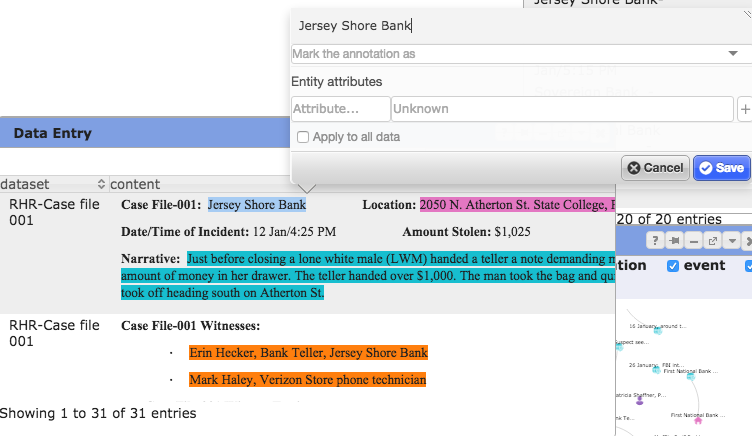
\includegraphics[width=\columnwidth]{03-System/img/annotation-1.png}
	\caption{Annotation in document view \label{fig:annotation-editor}}
\end{figure}

\begin{figure}
	\centering
	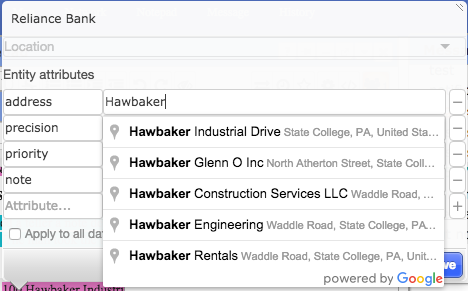
\includegraphics[width=\columnwidth]{03-System/img/annotation-location.png}
	\caption{Utility for location annotation \label{fig:annotation-location}}
\end{figure}

\subsection{Multiple coordinated views of annotated evidence}

CAnalytics supports multiple views for data visualization. Each view provides a means to schematize data, and thus an analytic perspective to understand data:
Timeline organizes data by time, so analysts can do time-sensitive analysis, such as the sequence of events and overlap between events.  The map visualizes evidence by location; with that analysts can do spatial analysis, understanding the proximity of events.  Node-link graph demonstrates the entities and relationships; connected entities are pulled closer by links and form into a cluster. This helps analysts easily decide the role of an entity: if an entity has a lot of connections in a big cluster, it is likely that it plays a leading role in the event. Finally, Table displays entity attributes and allows analysts to examine entities in detail.  

These views are generated automatically from user-created annotations. As shown in Figure~\ref{fig:interface}, when an annotation is created in the
document module, with attribute information about time, location, participants, and their
relationships, a new event is created in the timeline module, a new location is
created in the map module, and new people are created in the node-link graph
module with a typed edge representing relationships among the people (or new
edges are added to existing nodes). Different views are coordinated; that is,
when users do a filter on a piece of information in one view, related
information in other views will be highlighted. Filtering on different
views/schematization provides different analytic strategies; e.g. timeline
offers filtering by time, the map offers filtering by location, and node-link graph
offers filtering by related data objects. Based on the default view of the evidence,
users can continue to schematize it. For example, users can drag the nodes in
the node-link graph to make clusters. Users can also create a relationship in
the graph by drawing a link between two nodes and input relationship attributes.


\subsection{Information sharing and team awareness}

Annotations are immediately shared with collaborators. CAnalytics supports
real-time collaborative editing, similar to Google Tools. Users can open
several concurrent editors to collaboratively edit multiple annotations. Views
are shared together with hypotheses. Team members will then be able to
understand the hypothesis right in that visualization context. They can also
leverage that visualization and continue exploring by reorganizing the view, to
challenge, confirm, or refine the shared hypothesis. In this way, the team is
leveraging each other’s efforts and co-developing hypotheses beyond simply
sharing. CAnalytics has a number of awareness features, including animation of
data change, a notification system, a design we named “tool coordinator”, a
messaging tool, and a history tool. As mentioned before, annotations and data
objects created by collaborators are immediately shared, and updated in the
views. A fade-in and fade-out  animation in the views indicates the creation
and deletion action by collaborators. A notification system sends individual’s
actions to the team, in the form of a text box in the top right corner of the
workspace, keeping the team up to date with collaborator’s actions. To reduce
notification noise, instead of broadcasting whatever actions, we define a set of
rules to determine which actions will be notified. For example, the action that
creates an entity will be notified, but that re-layouts a view will not. Tool
coordinator refers to a small indicator on the tool menu bar, suggesting who is
working on the tool.

A messaging tool enables real time team communication. Chat history is persistent
for traceability. We design a “mention” feature—users can refer to created
entities and relationships in the workspace when they are composing a message.
We believe this will improve communication efficiency because analysts are often
observed to mention critical information entities in a face-to-face discussion.
When the message receiver hovers over the object, attributes of the object shows
up, ensuring that the team is referring to the same thing.

The system maintains a persistent log of time-stamped individual activities. A
history tool presents who did what to which object at when. Together with the
notification system, users who work synchronously can be informed of others’
activity continuously, and be aware of the bigger picture of the team’s activity;
users who work asynchronously will be able to use history to reconstruct
their work status and become aware of changes beyond the point of their last
interaction. Different from awareness features developed in existing systems
which are simply read-only text, the awareness information in our system is
closely integrated with the analytic environment. For example, data objects that
are changed and presented in the history view are clickable links. Users can
hover over to read detailed attributes and click to do a filter on the object.

\subsection{User activity log}

We designed our log schema based upon the work by \cite{Yi2007} and
\cite{Guo2016}. Our log focuses on high level activities that capture the
task the user intends to accomplish rather than their mouse movement. Actions
are categorized under the three top-level activities supported by the system:
data modeling, visual analysis, and hypothesis development. More detailed
actions, their definitions, as well as application-specific actions are shown in
Table~\ref{tab: log}.

\begin{table}
	\caption{Specification of user activities}
	\label{tab: log}
	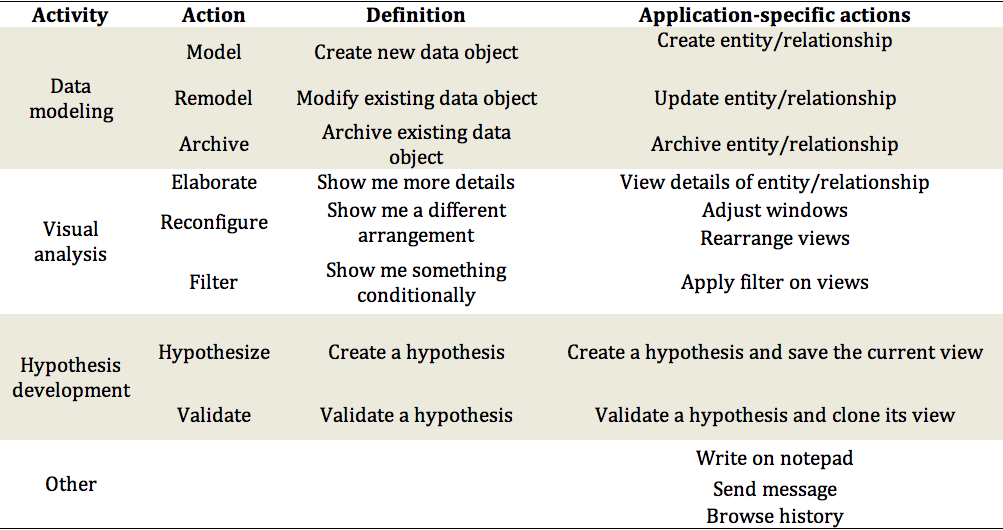
\includegraphics[width=\linewidth]{03-System/img/log_specification.png}
\end{table}


\subsection{Collaborative hypothesis development}\label{feature-hypothesis}

\begin{figure}
	\centering
	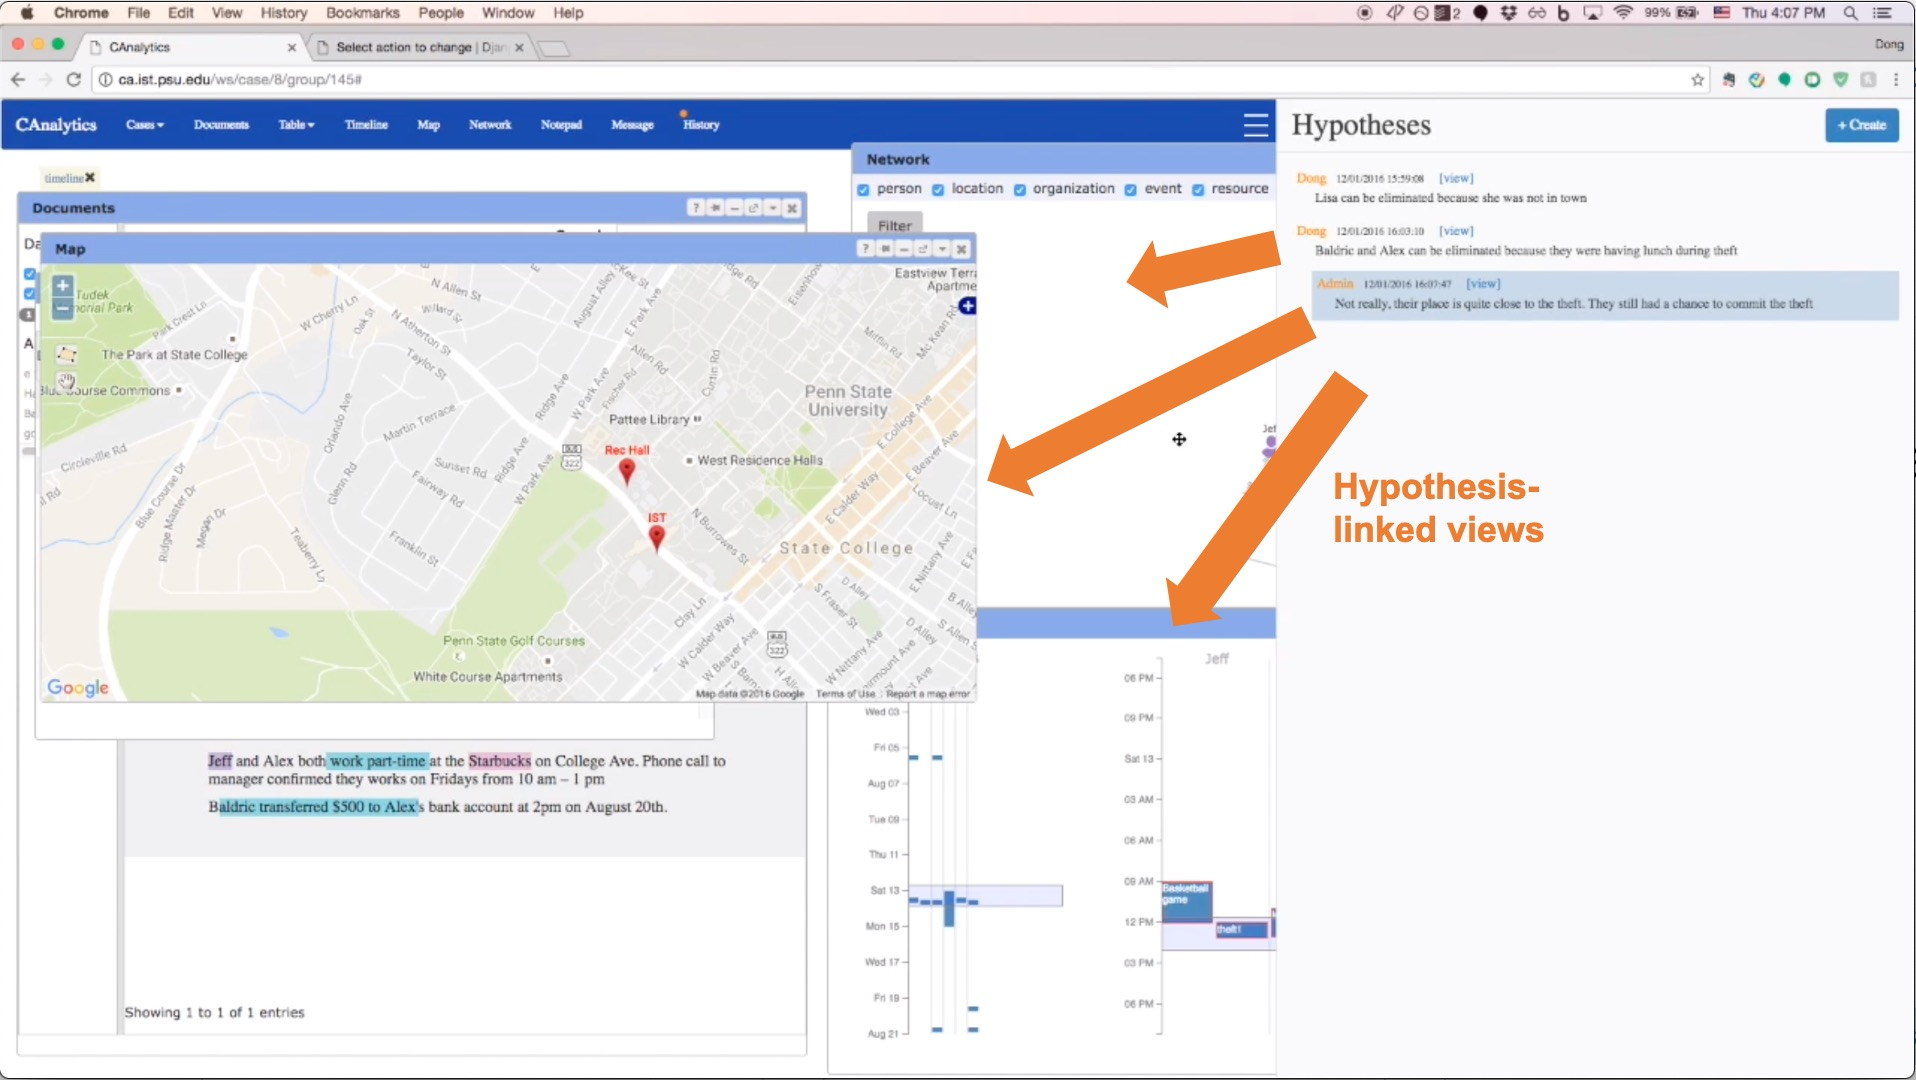
\includegraphics[width=\columnwidth]{03-System/img/hypothesis.jpg}
	\caption{Hypothesis development with linked views \label{fig:hypothesis}}
\end{figure}

All the above features are included in CAnalytics for the first classroom study. In study two, we developed CAnalytics2. A major addition is a structured approach to supporting collaborative hypothesis development. 

In study one with CAnalytics V1, teams put down their hypotheses and notes in a shared note editor. The editor is similar Google Doc, where text is synchronously shared. Hypotheses are shared in plain text, and no structured support is provided. Our first study suggests participants easily lost track of hypothesis development, and it was challenging to re-validate a hypothesis because the context in which it was created was gone. 

In CAnalytics V2, a hypothesis tool is developed as shown in Figure~\ref{fig:hypothesis}. At any time during the process of making annotations or analyzing visualization, analysts can create a hypothesis (with a textual note). In the meantime, the system will automatically record the ad hoc visualization state of all windows, including the data, layout, filtering conditions,etc., and save it together with the hypothesis. The hypothesis is shared with collaborators together with the bound visualization. Teammates who are interested in a specific hypothesis statement can restore the linked visualization. They can then continue to interactively explore the graph from which the statement was derived, either validating or deputing the previous hypothesis, or finding further evidence to propose a new hypothesis. Watch the video demo at  \url{https://youtu.be/pHqOukeg2KA}.
\section{Implementation}

\subsection{Managing team analytic states}
% 
% visualization state
% Shrinivasan2008b discusses managing visualization states in an analytic process


A particular challenge in implementing CAnalytics is effective management of dynamic states that occur throughout the information analysis process. Rather than simply displaying a static set of data as in many visualization systems, data and views in CAnalytics keep updating as analysts collect evidence, re-arrange views, and develop hypotheses. Each change generates a new ``state'' in the analytic system, which is like a ``shot'' of system dynamics that determine how a
system looks like. Managing the dynamically changing states is particularly important in collaborative analysis as states of all analyst's system should always keep synchronized; otherwise, a coordination breakdown could occur. 

\begin{figure}
	\centering
	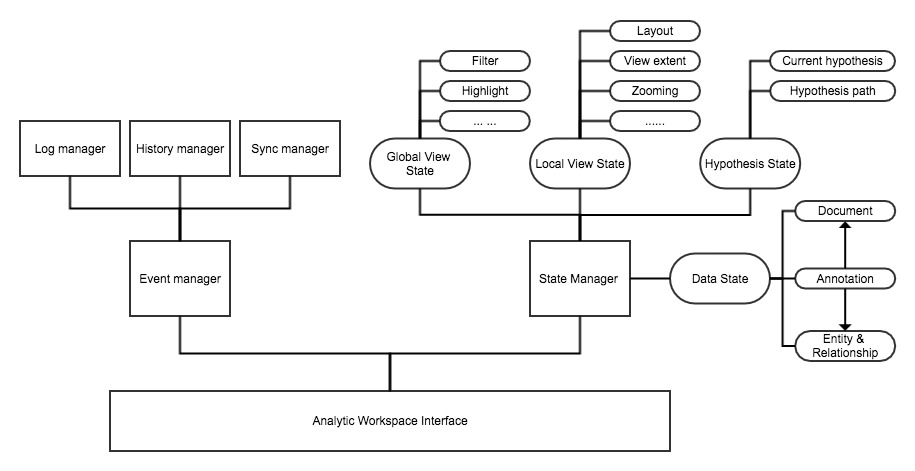
\includegraphics[width=\columnwidth]{03-System/img/architecture.jpg}
	\caption{State management in a dynamic system.\label{fig:architecture}}
\end{figure}

Aligned with the three major activities in information analysis, we create state managers for each activity, as shown in Figure~\ref{fig:architecture}. A data manager is in charge of the raw documents, user-created entities and relationships, and annotations that indicate in which part of a document is an entity created. A view manager controls the contemporary visualization state in the system. It includes a global view state and a local view state. The global state controls factors that affect all the views in the system. For example, a filter applies to all views so that the same subset of data is shown across views. A highlight determines which entities are on focus and underscore them in their representation. A local view state manages each individual visualization, including the position of the view in the workspace, the view extent, the zooming level, etc. 
Finally, the hypothesis state manager controls the current active hypothesis, as well as a path of hypotheses it builds upon. The path keeps track of the development of hypotheses and enables analysts to trace back. 


\begin{figure}
	\centering
	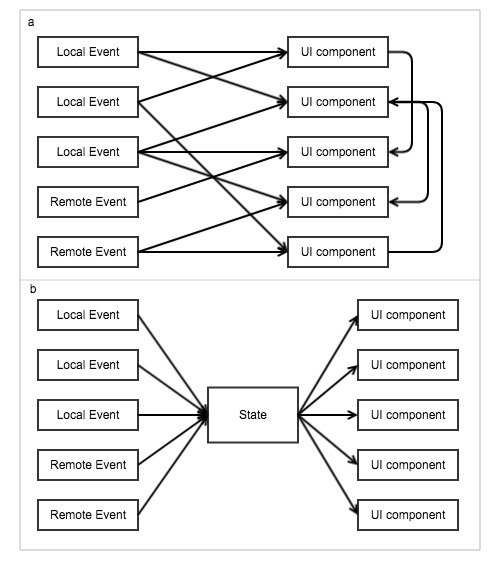
\includegraphics[width=.4\linewidth]{03-System/img/state_management.jpg}
	\caption{Diagrams showing two state management approaches. a) Event-driven approach: each interface component manages its own state and updates itself driven by events. b) Our approach: a central state manager takes care of all events and notifies interface components whenever there is a need to update.\label{fig:state_management}}
\end{figure}

User interactions drive the change of system states. These interactions are modeled as events and controlled by a manager. Depending on the type of events, the system includes a log manager, which saves events as system logs and team activity history, and a sync manager, which broadcasts events to the other systems in the team. 

After defining state managers and event managers, another challenge is to connect them to function as a dynamic system. A common implementation is event-driven:
each system component manages its own state and subscribes to events that change its state (e.g. \cite{hardisty2011geoviz}). This approach works for simple applications, but may be difficult to scale up in a complex system, especially a collaborative system in which there exist multiple sources that could change the system states. As shown in Figure~\ref{fig:state_management}a, a local
component can be changed by both a local (the user in operation) and a remote interaction (teammate). In turn, the
change of the local component could cause a change to another local component or
even a remote component. For example, a brushing interaction on the network changes
the state of the network (highlight entity nodes). The change of network state
in turn causes change to other views, for example, a reduced data view in the
map showing related locations to those highlighted entities. The state could
also be changed by a remote interaction when collaborators are sharing their
view, and, similarly, cause change to other views. To some extent, the groupware
developer no longer understands what changes a view, and the state of the
groupware would become out of control.

To address the issue, we employed a state-centered approach to make state control more structured and
clear. As Figure~\ref{fig:state_management}b shows, an event manager takes control of all events, whether
they are local or remote events. The event manager dispatches events to
different event handlers and makes changes to a central state manager. Whenever
the state changes, the state manager sends a signal to related interface
components, notifying them to update the view. This approach centralizes the
management of states, and the central state becomes the ``single source of truth'' \footnote{Single source of truth: \url{https://en.wikipedia.org/wiki/Single_source_of_truth}}. 
All user interfaces (including the ad hoc user and teammates) subscribe to \emph{the} state so that they will always be consistent. 

A typical event flow is demonstrated in Figure~\ref{fig:flow}. An event is triggered by a user
interaction. The event is sent to the Event Manager for processing. Depending on the nature of the event, the event manager may do three things. The event could change the local state directly (could be data, view, and hypothesis). The event is also sent to the history manager. It is saved as a system log for research purposes. There are also a set of rules that decide if the event is of interest to analysts. If it is, it is also saved as part of team history. Finally, the event is also passed to the sync manager if considered necessary. The sync manager then broadcasts the event to other systems in the team so that it can make exactly the same change in their state. 



\begin{figure}
	\centering
	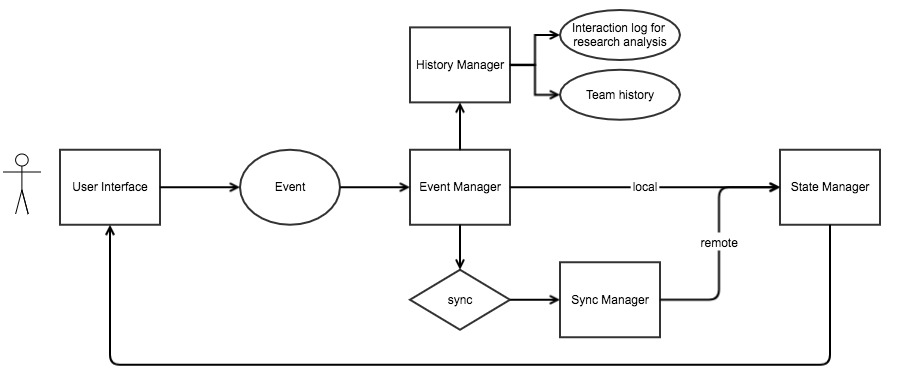
\includegraphics[width=\columnwidth]{03-System/img/flow.jpg}
	\caption{Event flow in a collaborative system.\label{fig:flow}}
\end{figure}

The system employs a standard three-layer web application architecture. The frontend is the application running in a browser that end users interact with directly. It is implemented in Javascript and HTML. We use PostgreSQL as the database. The backend server is implemented in Python/Django and Node.js. The Django server takes care of most REST API requests and reads and writes data into database. The Node.js is responsible for broadcasting data to systems in a team so that they can communicate with each other and keep their system state consistent. 
The tool takes advantage of the state-of-the-art HTML5 WebSocket technique to
realize real-time communication. WebSocket is a bidirectional, full-duplex
communication channel that operates through a single socket over the web. It is
part of HTML5 and provides a true standard for building scalable, real-time web
applications. Since most modern browsers implement the protocol as a standard,
no plug-in or other installation is required, which ensures convenient
accessibility to users. We intentionally keep the API server and sync server separate so that they are loosely coupled. Each server works on its own (the Django server will be like a single-user application on its own, and the Node server can be potentially plugged into other applications to enable collaboration). This approach opens an opportunity to develop the Node server into a \emph{service} that provides a more general collaborative functionality to standalone applications in the future. 

\subsection{Conflict resolution}

An important consideration in supporting collaboration is conflict resolution. A potential issue in CAnalytics is the addition of multiple annotations to the same text. CAnalytics supports multiple annotations by stacking them and marking the author and creation time of each annotation. The same issue may exist when users add multiple relationships to two entities. The node-link graph in CAnalytics resolves the issue by displaying multiple labeled links between two nodes (as in the node-link graph in Figure~\ref{fig:interface}). Therefore analysts can identify the potential conflicts and try to resolve them. It is also possible that it does not conflict at all. It may be two possible hypotheses due to uncertainty. In either case, this approach helps analysts identify potential issues. 

\subsection{View restoration and sharing}
Views in CAnalytics are handled as global views and local views. Global views refer to the window of each visualization, including which windows are open, the size of the window, and its position. Global views are saved and shared in JSON format. 

Local views are more complicated as they include all the nodes and paths of visualization. To restore the view back to the same layout when the analyst reopens it, positions of all individual nodes are saved. This means a large amount of data will potentially be downloaded and parsed when individuals intend to restore an existing view. This is still fine (though it probably would take a longer time), yet presents a challenge for real-time sharing. If we share the whole view state node by node in real-time, we need to pass a lot of data for each frame, and several frames per second for smooth animation. Obviously, this is not optimal. Instead of state sharing, we adopt event sharing. Only attributes of an event, for example, type of event (e.g. 'click', 'scroll'), the target of the event (which node is the event applied to), are shared. When partners receive the event, the event is applied to the visualization. Since each event has a deterministic effect, the partner will see the same animation and result of the visualization as the event source. By sharing only event and ensuring event effects are deterministic, we make possible real-time view sharing a smooth experience.

\chapter{The First Classroom Study}

\section{Problem Statement}

The first classroom study aims to evaluate our design Objectives One, Two, Three, and Five listed in Section~\ref{design-objectives}; that is, the study explores:

1. the effectiveness of supporting information analysis with an integrated workspace;

2. the effectiveness of structured data annotation and visualization;

3. the effectiveness of supporting activity awareness of the tool;

4. and how teams behave with the computing tool support.

\section{Setting and Method}\label{classroom-study-settings}

The setting for this study was an undergraduate course in an intelligence
training program at Pennsylvania State University. The program was designed to train students
to become professional intelligence analysts. A key requirement of the course is
to emphasize hands-on practice on team-based intelligence analysis.

 %\bvh{I would make a bigger point about the training in the tools that they
 %already had, they were sort of primed to not use a collaborative tool}

 % \bvh{separate the argument about waterfall and what students were already trained in and how it played out}
 During the first ten weeks of the course
 students learned several analytic techniques, including IEW (a technique
 to extract evidence and assess their values), ACH (a technique to evaluate
 multiple hypotheses against evidence), timeline analysis and network
 analysis, as well as state-of-the-art tools to implement these
 techniques, including Analyst's Notebook and PARC ACH. Students also practiced applying these
 techniques in two hands-on projects before our study. Students follow a typical ``waterfall'' workflow: they start with IEW to
 extract evidence from documents and model them into a structured format. With that data available, they start building analytic
 artifacts such as an ACH Matrix in PARC ACH, and a timeline and a network
 graph in Analyst's Notebook. Sometimes the process is not necessarily sequential, and they want to jump back to edit data when building analysis. Yet since the tools are separate and data within the tools are not sharable, the annotation activity and analysis activity are largely isolated and streamlined. 
 
 Most tools in use lack serious collaboration
 support (except that some teams use Google Doc to construct an IEW
 table). Analysts were unable to contribute simultaneously, an issue
 known as production blocking \citep{Diehl1987a}. Students often divide their work by tools: each person picks a tool, creates and analyzes an artifact
 with that tool on their own, and puts individual analysis together towards the end. This had the consequence that findings and
 hypotheses be made without integrating collective efforts and diverse
 knowledge. Analysts coordinated work by manually sharing documents
 or graphs through email or cloud storage service (e.g.~Dropbox),
 resulting in a scattered placement of results, requiring repeated manual
 resynchronizing to identify redundant or missing pieces of information,
 analysis of information, and analytic hypotheses. In summary, the students in our study had learned and practiced with tools lack of support for collaboration and were all aware of the shortcomings.

 %\bvh{do demographic stuff first}
 Of the 98 students enrolled in the course (from
 two sections), 73 consented to participate in the study. All of the 73 students
 held major in the program of Security and Risk Analysis. Most (75\%) of them
 were in the third academic year ($M=3.06 \text{ years}, SD=.44$), indicating that participants in
 our study had relatively advanced experience and knowledge in intelligence
 analysis. Participants' age ranged from 19 to 28 ($M=20.4, SD=1.18$). 77\% of the
 participants were male.

 Students were given a tutorial on CAnalytics a week before the project began.
 One of the authors walked through the features of CAnalytics, without enforcing or implying any strategic use of the tool. Students then accomplished a small case analysis at their own pace. During the week of the
 actual study, one author was constantly available to help with any technical
 issues. Although students were encouraged to make full use of CAnalytics, to
 ensure a naturalist environment students were always free to employ any other
 tools that they believed useful.

 \begin{figure}
 	\centering
 	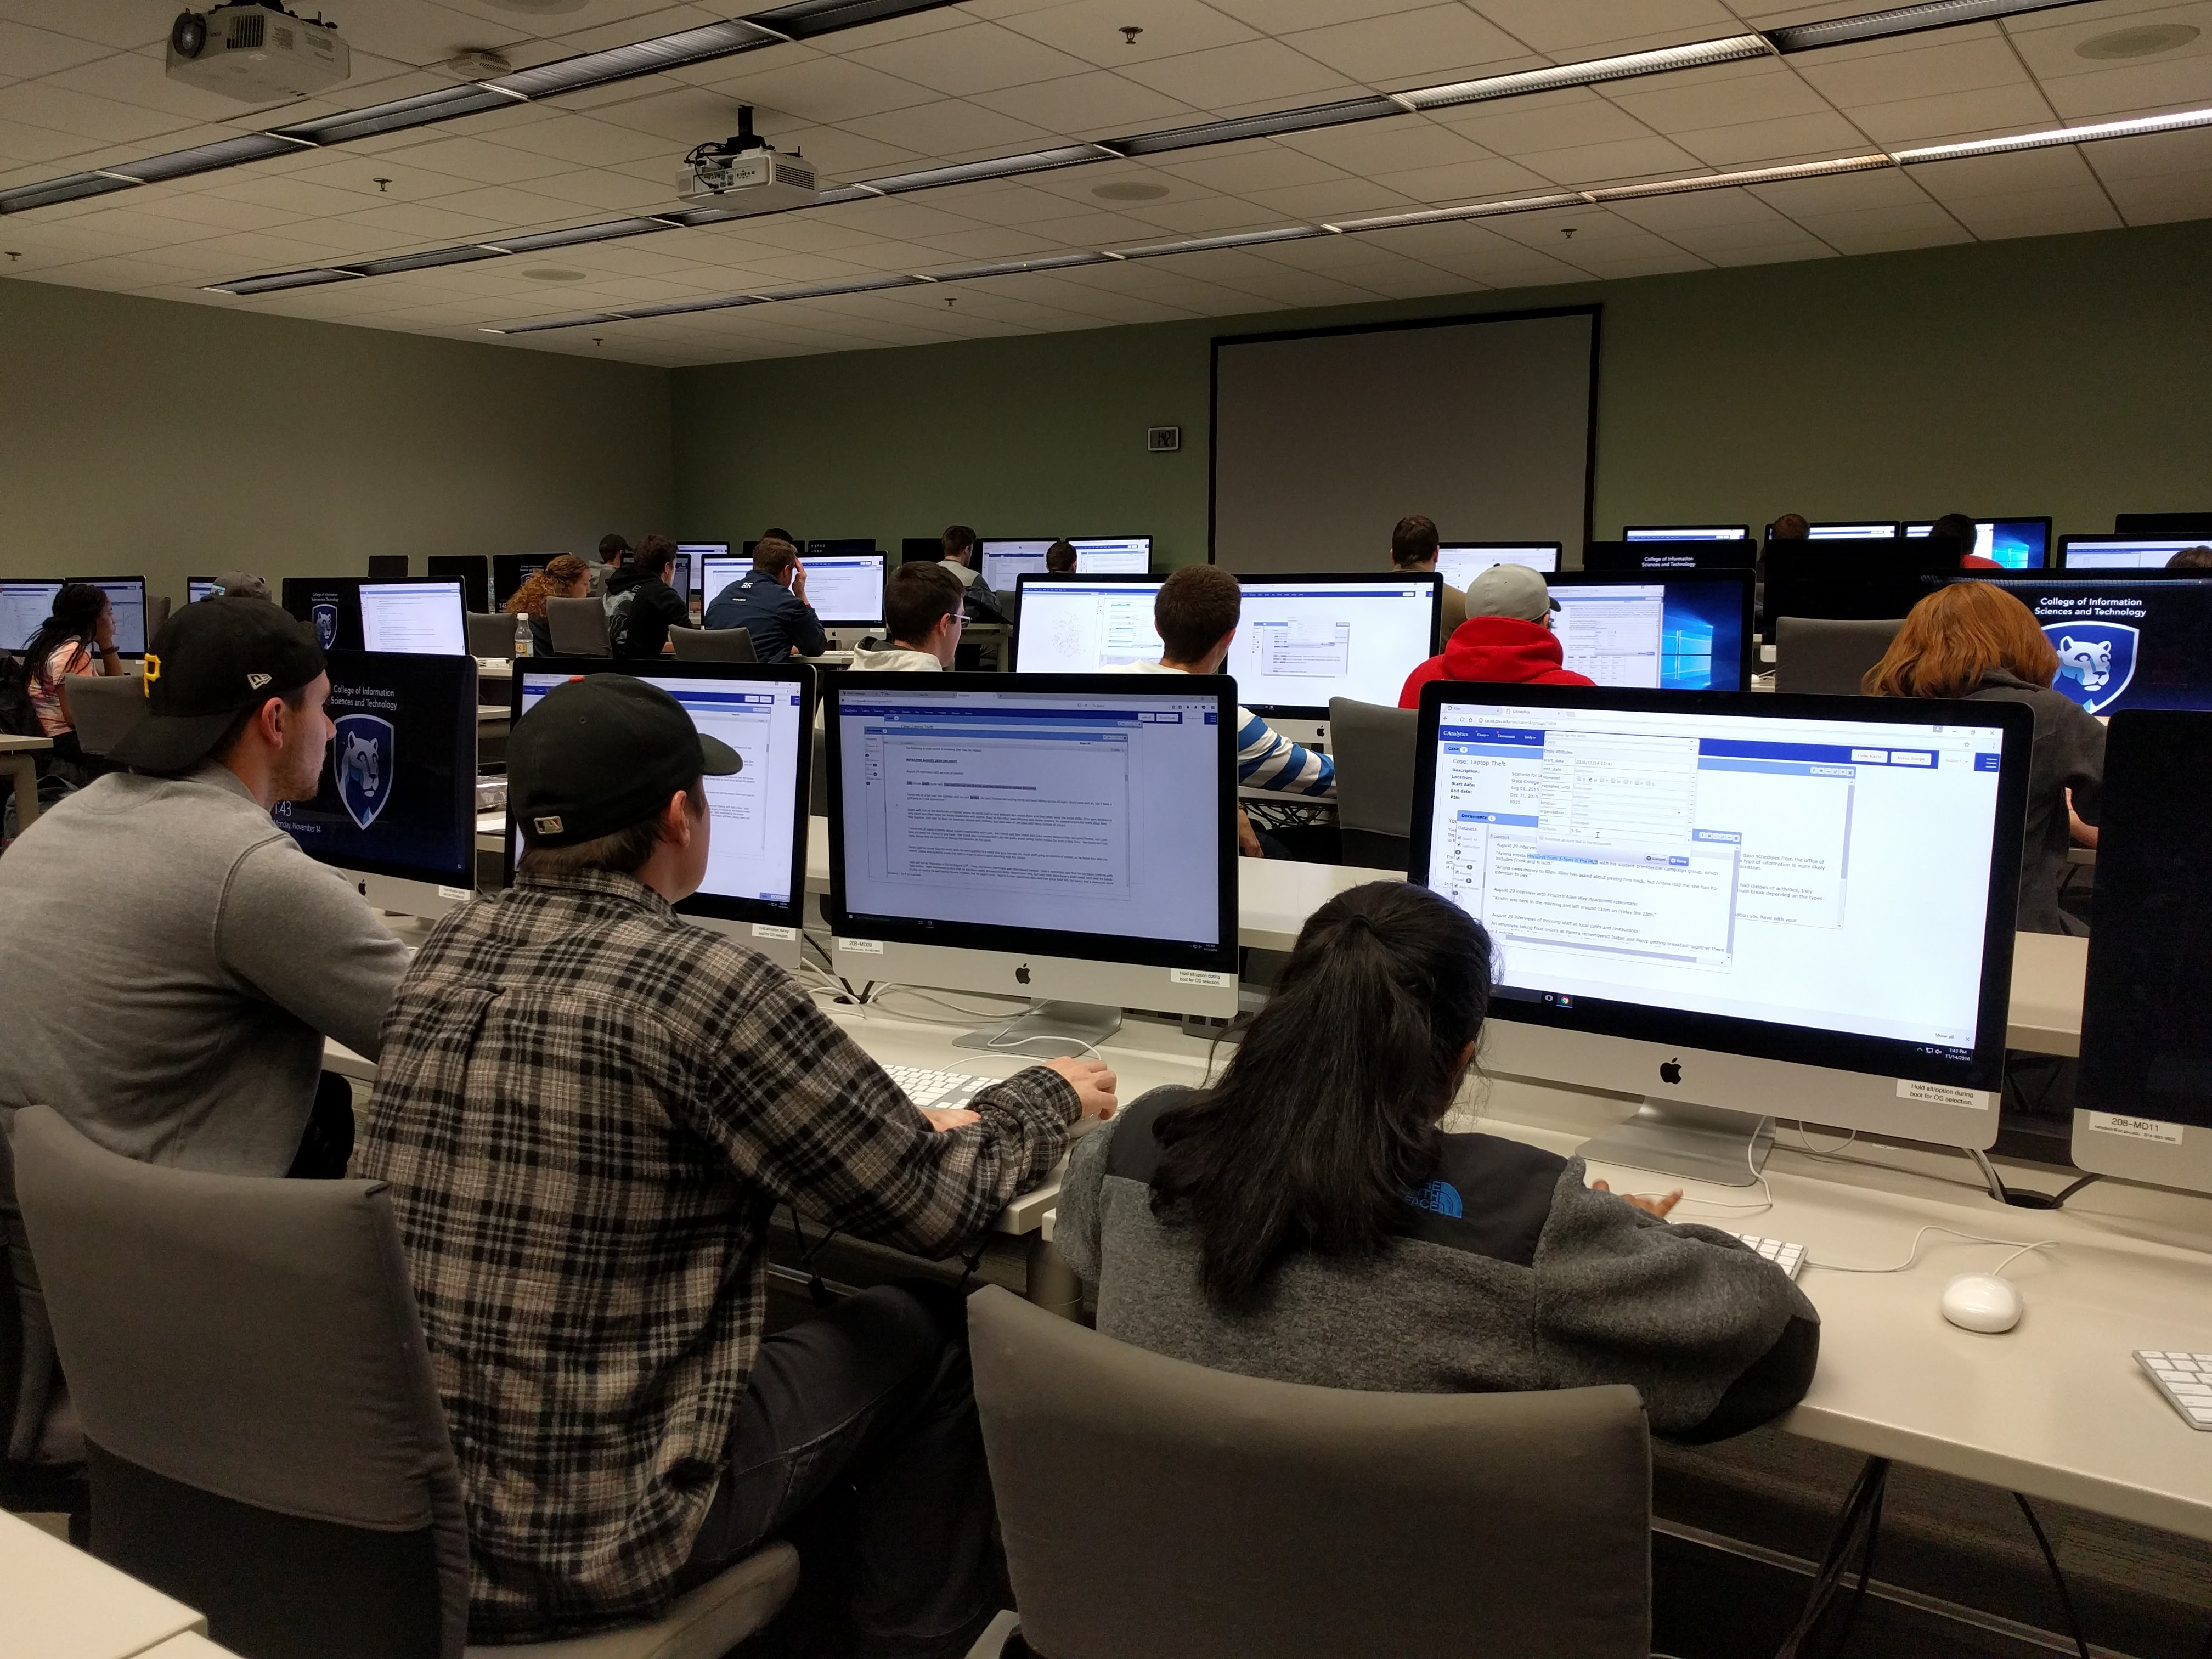
\includegraphics[width=3in]{04-Study_one/img/classroom_setting.jpg}
  \caption{Classroom setting}\label{fig:classroom}
 \end{figure}

Our study began on the 10th week of the course and lasted for one week. The
analysis that students performed on our tool was an investigation of a series
of bank robberies. The case and materials were fabricated by the course instructor. Teams
were provided a set of documents pertaining to seven robberies, including police
reports, witnesses reports, video records, and news media. The analysis was
designed to be open-ended, meaning that there was no single, definitive answer.
The instructor explained that the task was to simulate real world scenarios, in
which analysts always reasoned in the circumstances of uncertainty, ambiguity,
and complexity. The instructor told the students that he expected the analysis
to take around 6 hours, including in-class and outside-class work. At the end of
the project students were required to submit a team report, describing their
hypotheses, assumptions, conclusions, and supporting evidence. When in class, students used a 27-in Macintosh desktop (as shown in Figure~\ref{fig:classroom}. Students could use any equipment when outside class.

Students were randomly assigned into 25 teams (23 three-person teams and 2
two-person teams). Research suggested that group size be an important factor in
group collaboration, and two-person teams might behave differently from
three-person teams. We thus excluded data from the two-person teams in our
analysis in this paper. Also, from the log (and confirmed by their
questionnaire), we found that one team made little use of CAnalytics and opted
for other tools (Google Doc). Hence their data were also excluded. Our final data report includes the result from 22 teams.

We employed several data collection approaches. We administrated a post-study
questionnaire. The questions used a 7-point likert scale and included 9 items measuring an individual's
self-reported awareness, 7 items for
communication quality, 6 items for collective efficacy, and 3 items for perceived performance \citep{Convertino2011}. We also used NASA-TLX \citep{Hart1988} to measure cognitive load. The questionnaire
also included open-ended questions asking how the tool helped or impeded their
work. We captured user interactions with system logs. Instead of simply logging
low-level events like mouse clicks and keyboard strokes, we recorded meaningful actions such
as creating an annotation and deleting an entity. Finally, we reviewed team
reports and graded them as an indicator of team performance. Since the task was
open-ended, there was no single right answer. We constructed an assessment
rubric together with the course instructor by listing all possible hypotheses
and evidence from the documents, with a full score of 16. I and another researcher graded the reports independently. If the grades differ by
less than 2, an average is set as the final grade (14 out of 22 reports).
Otherwise (the rest 8 reports), the two graders review the reports together and
make an agreement.

\section{System}

The system, CAnalytics, used in this study includes all features described in Section~\ref{canalytics-features} except for the hypothesis tool. To sum up, CAnalytics includes an integrated workspace for data annotation and visualization, and enables real time sharing of user created data objects. It also includes a shared notepad which a team uses to put down their note and hypothesis. 
\section{Results}\label{study1-results}

Over the week, teams created 1805 entities and 1529 relationships in
total. The number of entities teams created ranged from 24 to 223 ($M=82,
SD=39.9$), and the number of relationships ranged from 7 to 237 ($M=69.5,
SD=51.0$), showing a large variety. The big range was related to different team data modeling strategy,
which will be discussed in detail later. While teams could work on the project any time, we found three intensive usage sessions from the interaction log: two were in class and one was before the team report deadline, outside of class.

CAnalytics was generally well-received by the students. An overview of
the related survey items (shown in Figure~\ref{fig:survey}) shows that students positively rated all aspects
of the tool except cognitive load, towards which they had a close to neutral feeling, which is understandable as the tool does not necessarily reduce the complexity and load of the task.  % \bvh{provide more detail here, don't just rely on the figure}

\begin{figure}
\centering
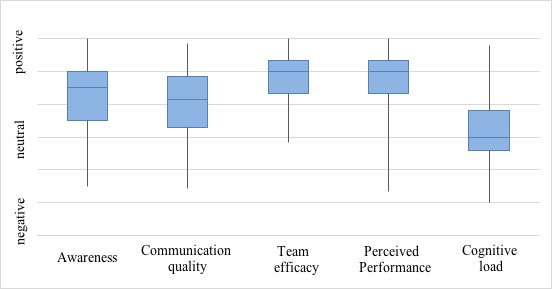
\includegraphics[width=\linewidth]{04-Study_one/img/survey_boxchart.jpg}
\caption{Survey responses (box shows Q1-Q3 and median; ends of whiskers show
maximum and minimum)\label{fig:survey}}
\end{figure}

\subsection{Filtering vs. Accretion}


\begin{figure}
	\centering
	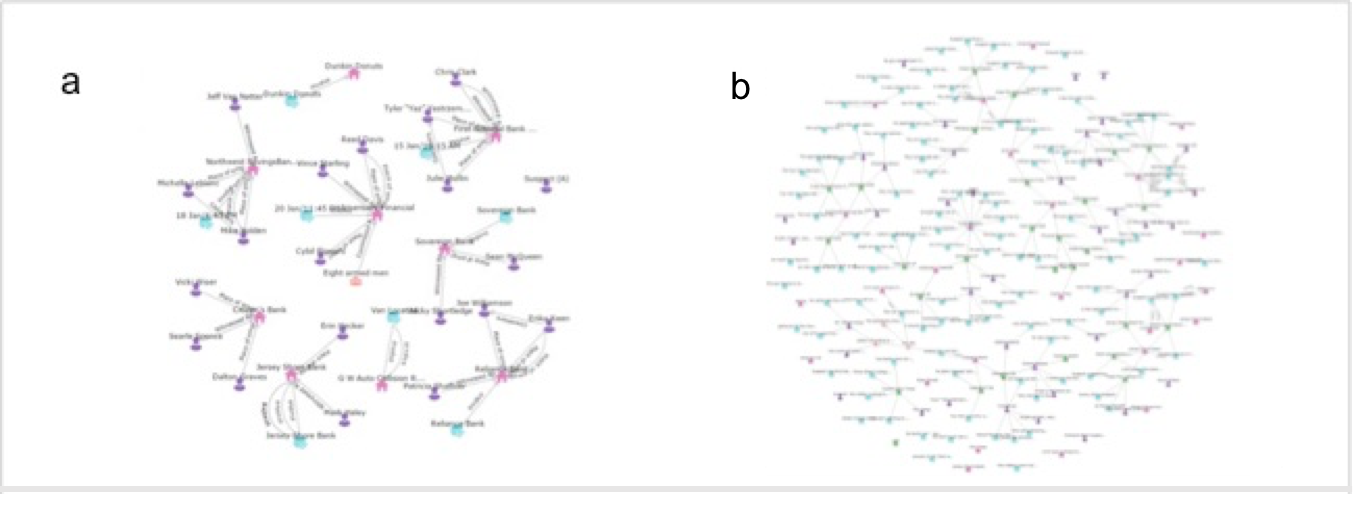
\includegraphics[width=\columnwidth]{./04-Study_one/img/network_accretion_filter.png}
	\caption{Network artifact comparison: filtering (a)
		vs.~accretion (b) \label{fig:network_accretion}}
\end{figure}

In examining participants' created data objects,
we noted a distinction between filtering and accretion
strategies, similar to what was reported in the paper prototype study \citep{Carroll2013}. Filtering is selectively modeling of data
and adding to an artifact. Users must decide what information is
relevant, and thus what is to be excluded, as well as what granularity
of information is to model. Filtering requires more team coordination
because teammates must reach a common ground of the current problem as
well as information needed to answer the problem. Figure~\ref{fig:network_accretion}a is an example of network built with filtering strategy. It only represented key information of robberies.

Accretion is an attempt to comprehensively represent the problem by
adding all information to an artifact. Users extract every fact from the
document, regardless of its immediate relevance to the problem.
Accretion requires less coordination as it is relatively mechanical note-taking. A disadvantage of accretion is that it can be time-consuming
to model all details and the produced artifact could be fairly complex.
An example is Team 108, who modeled
every step the suspects took, which resulted in far more entities (223) than
the average (82) and a more cluttered network view (Figure~\ref{fig:network_accretion}b). This accounted for the large range of entities created. Users also realized the problem. They reflected that they spent too
much time in detail events, and many did not help their analysis at all:

\begin{quote}
	\emph{I felt that after we were done annotating, we hadn't really accomplished
		anything and that we were no closer to solving the case than when we had
		started. In the end it didn't really help that we had annotated the
		data. (P86)}
\end{quote}

\subsection{Situational logic vs. Comparison}

\begin{figure}
	\centering
	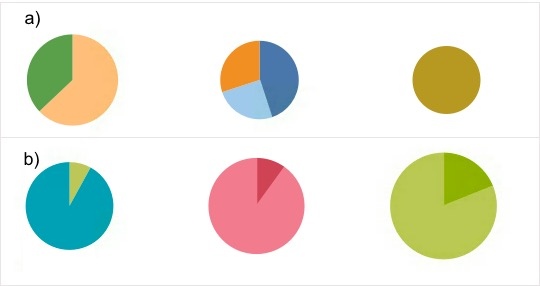
\includegraphics[width=\columnwidth]{04-Study_one/img/labor_division.jpg}
	\caption{Pie charts showing different labor division strategies. Each
		pie chart corresponds to annotations created by one team member. (a) Document-based
		collaboration. Each pie chart shows the documents a team member
		annotated, color coded by document ID. It is clear from the graph that the three team members work on different documents. (b) Entity-based collaboration.
		Each pie chart shows the entity types a team member created, color
		coded by entity types. It is clear that the three team members create different entity types across documents.
	\label{fig:labor_division}}
\end{figure}

We examined the patterns of the annotations teams created. We saw a clear distinction in terms of how teams divided their work in creating annotations. Seven
teams created annotations with a document-based pattern: each teammate focused on their own set of documents and made concrete detailed annotations.
(as shown in Figure~\ref{fig:labor_division}a). Individuals consider the known facts of the current document and seek to identify the cause-effect relationships of this document. We take the term \textit{situational logic} from \citep{Heuer1999} to describe this pattern, in which teams start hypotheses ``with concrete elements of the current situation, rather than with broad generalization that encompasses many similar cases'' (p.32). The team relied on partners to identify and share useful information within their assigned documents. The failing of this
strategy is thus in case an individual fails to identify or convey
evidence in the document, the team may overlook or misunderstand the information
altogether.

Four teams followed a different strategy. Instead of dividing by documents, they divided work by entity types: each individual went through all documents but only focused on and annotated
entities of certain types, e.g.~teammate A only annotated persons and
teammate B annotated locations (as shown in
Figure~\ref{fig:labor_division}b). This is known as a \textit{comparison} strategy \citep{Heuer1999}. When analysts recognize two entities as comparable, they use the known entity to fill gaps in their understanding of the present entity. They build connections between two entities, make analysis of similarities and distinctions. Different from situational logic, comparison interprets the present evidence in the context of precedent elements in other documents, and they could examine entity patterns across multiple documents simultaneously. The challenge is of course to decide whether two entities are truly comparable. There is a tendency to conclude two entities are equivalent simply based on the fact that they are equivalent in some aspects. When individuals fail to convey the assumptions made in the comparison, it could mislead the whole team's reasoning.

The rest (eleven) of the teams did not show specific labor division
patterns. Teammates were reading and annotating
the same document concurrently. Concurrent analysis of a document was challenging if not impossible with paper documents or traditional tools but is possible because the groupware allows them to see new annotations by others in
real time and to build on top of other's annotation. Figure~\ref{fig:close_collaboration}
shows an example where one team worked on the same document simultaneously.
The three team members exhibited high synchronicity in which document to
analyze, which we believe was not by accident. This has the advantage that
teammates are always on the same page and can discuss hypotheses
throughout the analysis process. A problem with this approach is scaling. It demands a lot of individual efforts since each teammate is required to analyze all documents and entities and constantly switch between individual work and collaboration work. As data size increases and analysis time tightens, the team may not afford this approach.


\begin{figure}
	\centering
	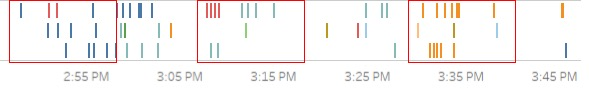
\includegraphics[width=\columnwidth]{04-Study_one/img/close_collaboration.jpg}
	\caption{Graph showing the timeline of one team creating annotations.
		Each row corresponds to one team member. Each bar represents an
		annotation, color coded by document ID. The red blocks highlights the
		periods when teammates worked on the same documents
		simultaneously.\label{fig:close_collaboration}}
\end{figure}



\subsection{Inferential connection vs. Factual discrete}

\begin{figure}
	\centering
	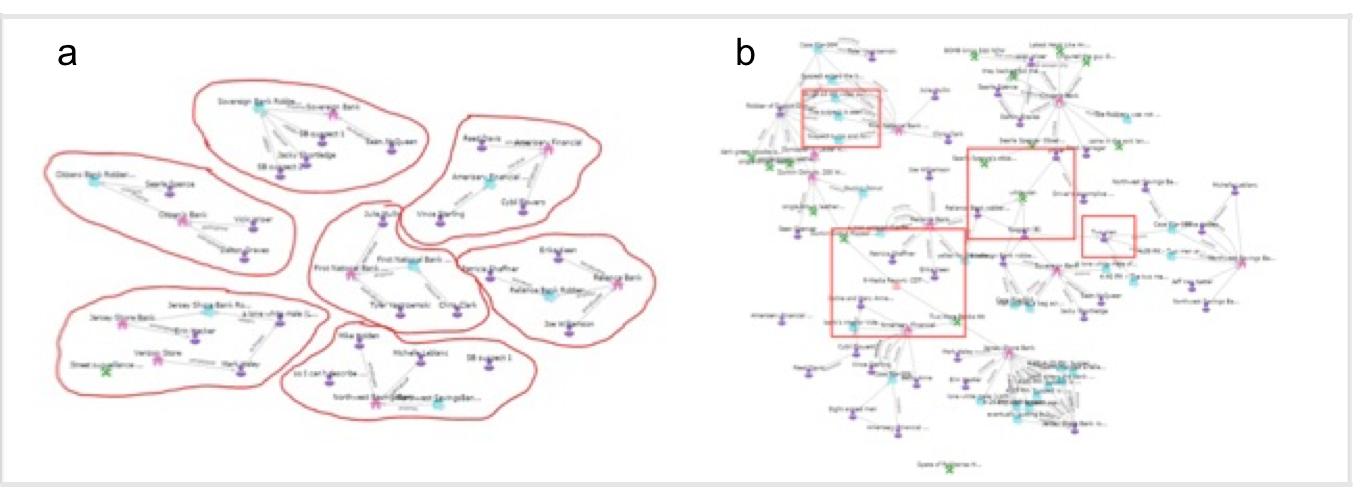
\includegraphics[width=\columnwidth]{04-Study_one/img/network_cluster.png}
	\caption{Network artifact comparison: separate clusters (a)
		vs.~connected clusters (b). The parts highlighted in red squares in (b) are key
		evidence that connects clusters\label{fig:network_cluster}}
\end{figure}

When examining the network artifacts participants created, a clear distinction exists in the shape of clusters. Networks from eight teams consist of discrete clusters
(Figure~\ref{fig:network_cluster}a): Nodes within a cluster are
connected. They are factual entities and relationships extracted from one single robbery case.  Each cluster is self-contained, with no links in between. In contrast, six other teams created networks that consist of connected clusters. Nodes and links within a cluster are similar to ones in the discrete cluster, but these clusters are connected through an
inferential link (Figure~\ref{fig:network_cluster}b, marked in red in the graph).

The differences in network artifacts relate to how teams annotated and represented entities in documents, especially in circumstances of incomplete, ambiguous information. For example, we have the following document snippets:

\begin{quote}
	Case 1: Suspect is shown running down N Atherton and jumping the passenger side of a white van
	
	Case 2: [...] we all watched as the guy ran around the parking lot. I went to the door and saw him jump into a white van of some type
\end{quote}

In both cases, suspects are associated with ``a white van''. Yet with only that information we are not able to conclude the white vans are the same one. That's the \textit{uncertainty} analysts must consider, and must properly represent. We see three types of annotation in team's network artifacts, as shown in Figure~\ref{fig:van}. In figure a, the vans are treated as two separate entities with the same name. It keeps their relationship open to question, yet analysts might have difficulty in identifying this hidden link in later analysis, especially when the network scales. In figure b, analysts merge the two vans into a single entity. This representation makes the connection apparent, yet misses the uncertainty information, which could mislead teammates. We found some teams using the notepad tool in CAnalytics to complement that the link is hypothetical. In figure c, vans are perceived as two entities but connected with a link, which is often labeled with text like ``hypothetical''. 

The three representations reflect different strategies in handling uncertainty. In figure a, analysts are more ``negative'', or conservative, toward uncertainty. They avoid bringing in any hypotheses during the stage of annotation, so as to avoid any bias confirmation in the analysis. In contrast, analysts in figure b are most ``positive'' with uncertainty. If they believe the inferential connection is a high possibility, such representation helps them identify important patterns and make quick decisions. In general, figure c appears to be more reasonable. It represents the connection while preserving the uncertainty, yet requires more annotation efforts. 


\begin{figure}
	\centering
	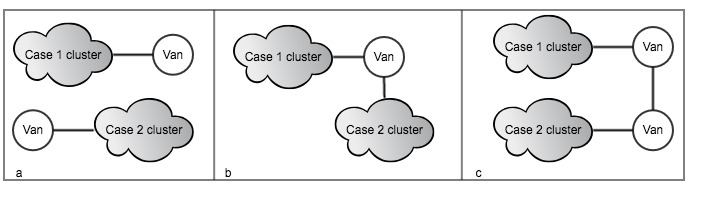
\includegraphics[width=\columnwidth]{04-Study_one/img/van.jpg}
	\caption{Three different representations of uncertainty for entity relationships\label{fig:van}}
\end{figure}

However, it does not mean these teams believe these cases are irrelevant. In fact, these teams still discussed connections between robberies in their report.
It turned out that these teams documented possible relationships in the notepad tool in the form of free text, separate from the network graph. That is, these teams distinguished information content and synthesized them in different artifacts.

%\bvh{how about this - same comment, outline what it means in a sentence and then tie them together like you do in the next sentence.}

By comparing these two types of networks, we found that links within a cluster were typically
\emph{factual} relationships modeled from raw documents (e.g.~a white van was
witnessed at a location), and links between clusters were often
\emph{inferences} beyond literally documented (e.g.~a white van at location A
is the same van witnessed at location B). Teams creating separate
clusters represented only facts in the network and held evidence of
uncertainty in a separate artifact. One advantage of distinguishing
facts and inferences is that teams can always be aware of assumptions made when
making a conclusion. And since all inferences are held in one place,
teams are forced to confront them and review their uncertainty
iteratively in the process. However, the strategy also adds difficulty
to analysis as analysts may overlook or fail to combine evidence
scattered in different artifacts.

% place table simply for paper layout
% % Please add the following required packages to your document preamble:
% \usepackage[table,xcdraw]{xcolor}
% If you use beamer only pass "xcolor=table" option, i.e. \documentclass[xcolor=table]{beamer}
% \usepackage[normalem]{ulem}
% \useunder{\uline}{\ul}{}
\begin{table*}[]
\centering
\caption{Subject feedback of awareness aspects}
\small
\label{tab:awareness}
\begin{tabular}{p{3cm}p{14cm}}
\rowcolor[HTML]{9B9B9B}
\multicolumn{1}{c}{\cellcolor[HTML]{9B9B9B}\textbf{Element}}                           & \multicolumn{1}{c}{\cellcolor[HTML]{9B9B9B}\textbf{Example}}                                                                                                                                                                                                                                                                                                                                 \\
\rowcolor[HTML]{C0C0C0}
\begin{tabular}[c]{@{}l@{}}Social awareness\\ \emph{who is present?}\end{tabular}             & CAnalytics helped me stay aware,of my teammates activities because I could see who was logged on in the top,right corner (P123)                                                                                                                                                                                                                                                              \\
\rowcolor[HTML]{EFEFEF}
\begin{tabular}[c]{@{}l@{}}History awareness\\ \emph{Who has done what?}\end{tabular}         & The way you are able to view when and where your teammate made or updated annotations/information was the key to staying aware of what your team has done. It is a great tool in respects to that. For example, I was able to view the changes my team made while I was not using the CAnalytics tool at the same time they were using the history tab. (P171)                               \\
\rowcolor[HTML]{9B9B9B}
\begin{tabular}[c]{@{}l@{}}Information awareness\\ \emph{What is being changed?}\end{tabular} & CAnalyitics was very helpful in keeping us updated on what was being changed/noted/amended by whom and when. This was very beneficial for staying on the same page and knowing what changes were being made so no one individual was out of the loop. (P157)                                                                                                                                 \\
\rowcolor[HTML]{EFEFEF}
\begin{tabular}[c]{@{}l@{}}Action awareness\\ \emph{Who is doing what?}\end{tabular}          & I liked how you could always see what your teammate were viewing on the website. For example I was working on the bluf when my teammates were working on the network part of the program. If I were to come across a piece of information that I thought might be helpful to them I would just tell them. My teammates did the same thing in return. (P51)                                   \\
\rowcolor[HTML]{C0C0C0}
\begin{tabular}[c]{@{}l@{}}Intention awareness\\ \emph{Who is going to do what?}\end{tabular} & CAnalytics showed what tab {[}tool{]} my teammates were working on which helped me be aware of what they were working on. For example, if I saw that one of my teammates was on the network tab, I knew that they were attempting to connect the information that was relevant to one another.,I would then be able to mention any new findings I had that could influence their work (P160)
\end{tabular}
\end{table*}



On the contrary, in connected-cluster networks, facts and inferences overlaid in one artifact together drive the layout of the
network, are better synthesized, and give analysts a clearer picture in one place. Teams may discuss and evaluate the level of uncertainty of inferences to decide whether to add them to the
network. This strategy makes analysis more interactive among teammates:
they need to negotiate, evaluate, and reach consensus on the value and
validity of inferences. However, a problem with mixing facts and inferences is, to some extent teams might forget whether a
link is factual or inferred, and ask whether conclusion derived
from the visualization can be trusted under uncertainty.


\subsection{Interleaving data annotation and analysis}\label{interleaving-data-annotation-and-data-analysis}

%\bvh{you need the reason why this is interesting...i.e. evidence of these behaviors shows that the tool was used collaboratively}

%\bvh{also what exactly do you mean by interleaving ... you should probably give an example or something??? maybe not, up to you}

We examined the pattern of data modeling and analysis first by
qualitatively looking at a visualization of the entire interaction log
(e.g.~Figure~\ref{fig:interleaving}a shows one team's interaction). All teams
worked intensively on data modeling as they started off the project.
This was the phase when teams were getting themselves familiar with the
documents and made initial annotation input into CAnalytics. Starting from a certain
time point, all teams started analysis on visualizations,
followed by frequent transitions between data modeling and analysis. 11
teams started data analysis in the first usage session, while the other
11 teams had this transition in the second usage session. On average,
the transitions occurred in 47.6 minutes after the project began. The earliest transition occurred in 14 minutes after the team started the project, and the last team
had the transition around 104 minutes, later in the second session. We
also found performance differences among teams that started analysis
early and those late. Teams that started analysis in session one had
higher performance ($M=8.6$) than teams that started from session two
($M=6.7$), although the difference was not statistically significant.

The fact that participants returned to making annotations after analysis
indicated that they did not wait to start analysis till they had
finished modeling. Indeed, the activity of data modeling and data
analysis were highly interleaved throughout the project (as shown by the interleaving color bar in Figure~\ref{fig:interleaving}a). Participants switched from
one activity to the other activity frequently. The state transition
diagram (Figure~\ref{fig:interleaving}b) demonstrates the interleaving in an aggregated way, in which we
encode the number of transitions as the width of a link. This result
confirms our design expectation that data modeling and analysis should
not be supported as separate staged activities, and that an integrated
environment should streamline the workflow.

\begin{figure*}
\centering
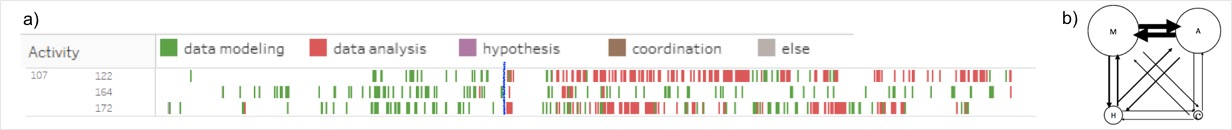
\includegraphics[width=\columnwidth]{./04-Study_one/img/intertwined.jpg}
\caption{(a) Visualization of interaction logs of Team 107. Each row of
colored marks indicates the sequence of top-level activities a
participant performed. (b) State transition diagram of interaction logs of Team 107. Each node is an activity, whose size represents the time spent on it (M: data modeling; A: data analysis; H: hypothesis development; C: coordination); a
link represents a switch from one activity to another, whose width
encodes the number of switches. We see highly frequent transitions between data modeling and data analysis \label{fig:interleaving}}
\end{figure*}




\subsection{Collaboration and
awareness}\label{collaboration-and-awareness}


One recurring theme in the subject feedback we collected was that the
collaboration features were helpful for solving the problem. In the survey
88\% of the students positively rated their
group awareness. Participants appreciated that the tool complemented
traditional analytic tools, describing CAnalytics as Analyst's Notebook with real-time
synchronization features similar to Google Docs, or described it as Google Doc with added visual analytics. To quote one participant,
\emph{``CAnalytics is like an analysts notebook that multiple people
could work on at once {[}\ldots{}and{]} an analysts version of a Google
Doc'' (P65)}.

Participants reflected that they could now contribute simultaneously
without concerns of interference and could
have everything in one place instead of manually sharing documents via a
cloud service.

\begin{quote}
\emph{It was much easier to coordinate as a team with CAnalytics because we
could all work on the same system at the same time. Without CAnalytics,
we were forced to do the work separately and compile all the work onto
one system after we had finished. (P156)}
\end{quote}

Students also reported that being able to see teammate's status made the
task more motivating and engaging:

\begin{quote}
\emph{During class I wasn't sure if my teammates were doing work for that
class or another thing but then seeing their dot {[}tool indicator{]}
switch between applications on the software and updates pop up on my
screen I knew they were doing work for 231. (P141)}
\end{quote}

\begin{quote}
\emph{The fact that you can see what other teammates are doing and they can
see what you are doing creates a sense of accountability in terms of
separating the workload. (P51)}
\end{quote}

The motivating effect of awareness might account for, at least partially,
the fact that teams were participating equally. We measured the equality of
participation in terms of the number of created entities and time spent on
CAnalytics. We refer to Olson \cite{Olson2017} in calculating equality: one
minus the variance of proportions times 100 (for better readability). Thus
the score ranges from .67 (when only one person contributes in a three-member
team) to 1.00 (when everyone participated exactly equally), and a higher
score indicates higher balanced participation. The resulted equality of
created entities and time was .96 and .99 on average respectively. This
indicates participants contributed fairly evenly.

Another repeated theme was the awareness features helped assure all teammates were executing
the team plan. Participants reflected on their experience that a common
team breakdown was a misunderstanding of the team plan, and that they did
not realize the misunderstanding until everyone had spent significant efforts
finishing their ``perceived'' job. CAnalytics made plan execution assured
because they could always see where teammates were working and what they
were generating; and if anything unexpected happened, they could communicate
immediately rather than at the end of the project.

Participants reported many other instances of awareness they realized
using CAnalytics. We categorized them based on the element of awareness,
or the essential problem of awareness of \emph{what}
\citep{Schmidt2002}, into social awareness, information awareness,
action awareness, history awareness, and intention awareness, as shown
in Table~\ref{tab:awareness}.


\begin{table}
	\caption{User reported awareness}
	\label{tab:awareness}
	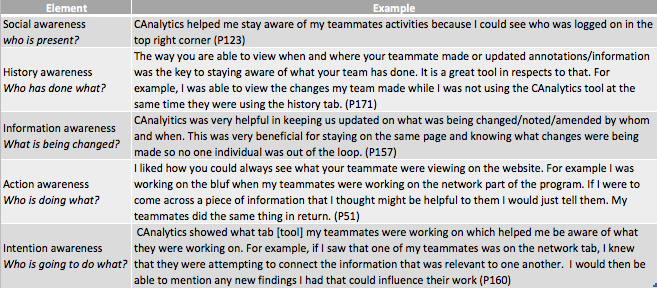
\includegraphics[width=\linewidth]{04-Study_one/img/awareness.png}
\end{table}


When asked what features helped them stay aware of team activities, 28
participants mentioned the tool coordinator, 24 mentioned the
notification system, 19 mentioned the history tool, 14 mentioned the
real-time update of user-generated data, 12 mentioned the collaborative
editor, and 7 mentioned the message tool. Although the number of mentions
does not simply indicate tool usefulness, it suggests users were explicitly aware of these awareness features and appreciated their support.


Students' positive feedback on awareness was further corroborated by
interaction logs. For example, we measured the number of entities
accessed by other collaborators. While data
generated by users is automatically shared, it is up to collaborators
whether to read/edit the shared information or ignore information altogether.
The log showed that on average, 77.6\% of the created entities
were \emph{read} by at least one other teammate. Further, We measured how
many entities were \emph{edited} by collaborators, a phenomenon we argue
requires higher awareness, because the collaborator must not only realize
the creation of the entity, but also understand its content. We
defined \emph{peer editing}, manipulated as the ratio of editing 
entities over editing those created by oneself. We found that all teams
edited collaborator's entity objects, with a peer editing value equal
to .83 ($SD=.45$). The result suggests that teams had little difficulty
accessing and modifying partner's created data objects.

%/bvh{I don't understand this paragraph...what are you trying to say...that they would like to have a shared space?}
One major critique is the lack of support for sharing intermediate analytic
insights. Insight is revealed and contextualized by a specific arrangement of views, e.g.~a reduced data view of interest through filter, a highlighted entity representing the analytic focus, and a clustering layout of network to demonstrate a specific relationship. While teammates share the same data pool, they are likely to have different views of data, and thus different \emph{interpretations}
toward the data. A dynamic view together with its interpretation represents
user's intermediate analytic status. Sharing these insights could inspire team analysis \citep{Gotz2009d}. With CAnalytics
participants complaint that they could not easily make such communications. The team could \emph{``be
looking at the same information but arranged in completely different
ways'' (P131)}.

\subsection{Interaction with team performance}

To systematically evaluate factors that influenced team performance,
we conducted a multiple linear regression between team performance
as the dependent variable and team collaboration characteristics
(i.e.~equality of entities and time respectively, peer editing, number of entities created, shared
entities, switch time from data modeling to analysis) as independent
variables. We treated a team as a system \citep{Henman2003b} and modeled team-level
relationships.
The relationship of individual level variables (e.g.
survey items) could not be simulated with regression directly because data within a team was interdependent. The analysis was performed using \emph{R} \citep{R2016}.

The result is shown in Figure~\ref{fig:regression}. The regression model was found to be statistically significant ($F(5,16)=4.58; p<.01$), with an R squared equal to .59, meaning 59\% of the variability in team performance was explained by the model. Five team-level variables contributed significantly to the prediction of team performance. The model suggested that balanced contribution of entities predicted higher team performance scores ($\beta=45.79, p<.05$), but balanced participation time did not show such effect. More peer editing led to better performance ($\beta=3.89, p<.01$), implying that analysts should be encouraged to model data as a team, and to remodel other's entity objects as needed. Longer elapsed time before a team started analysis (\emph{switch time} in the figure) predicted lower performance ($\beta=-.05, p<.05$), which suggested that teams should shorten the time of pure data modeling and start analysis earlier. A larger number of entities teams created also predicted higher performance ($\beta=.03, p<.05$). This can be interpreted that teams providing sufficient model input did benefit from system support. However, we are not ready to claim more entities are always better because we should also be cautious that entities irrelevant to the team problem bear no value to team analysis, as discussed beforehand. Somewhat surprisingly, the number of shared entities negatively predicted performance ($\beta=-8.99, p<.05$).
%\bvh{hard to understand this sentence...not sure how to rewrite it.}
We considered this might also relate to the issue of entity value: sharing entities without relevance to the team problem leads to reduced team efficiency and creates distraction, which in turn would lead to worse team performance. Another possibility is that teammates may not necessarily access all entities their partners created. The theory of Transactive Memory \citep{Wegner1987} suggests that teammates do not have to know everything in the team but should know ``who knows what''. Individuals specialize in their own field (e.g. one specializes in event analysis while another in social relationship examination) and reach for collaborators when other knowledge is needed. In such cases, common knowledge in shared entities would actually be redundant. Individuals should stay aware of the creator of an entity, but not necessarily the content of every entity.

\begin{figure}
\centering
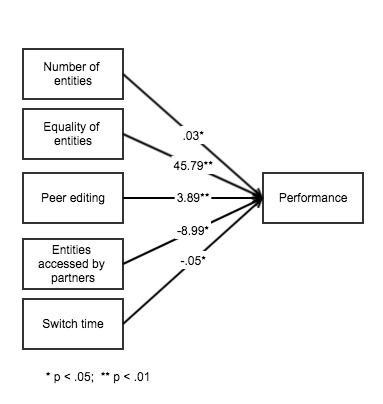
\includegraphics[width=0.6\columnwidth]{04-Study_one/img/team_analysis.jpg}
\caption{The relationship between collaboration characteristics and team performance.\label{fig:regression}}
\end{figure}

\section{Discussion}\label{discussion}

The goal of the study is to understand and support an interleaved, collaborative workflow in information analysis by evaluating tool usage in a natural
environment over multiple usage sessions. Our work responds to calls for an
integrated environment in the intelligence community as well as other data
intensive domains \citep{Shah2014i, Chen2016, Vision2015, Amershi2015, Ware2012}.
The system builds upon prior empirical studies (e.g. \cite{Carroll2013,
	Borge2012,Kang2011,Chin2009}) and embodies their design implications in our
tool. The study also complements research that only tests tools in short term
lab studies (e.g. \cite{Convertino2011,Goyal2016,Hajizadeh2013}) by
investigating tool usage over multiple usage sessions.

This study adopts an \emph{analyst-centered design} approach. A critical
requirement of developing tools that meet user needs is to understand their
needs and practices. When these needs and practices are specialized (as is the
case in intelligence analysis), it is particularly important to include the
target user population in the design process \citep{Scholtz2014}. Our classroom
study provided an opportunity with deep access to analysts in training. These
analysts have been trained with knowledge and skills of intelligence analysis,
and have experience with state-of-the-art analytic tools such as Analyst's
Notebook and PARC ACH. In their reflections, participants often compared
CAnalytics to those tools. Their multi-session usage of CAnalytics also allows
them to adapt to the tool and learn to appropriate it to the best of their team
purpose \citep{Stahl2006}. Therefore, while their feedback is admittedly not the
same as an experienced professional, their feedback does provide a deeper
insight into strengths and weaknesses of the tool.

The study provides encouraging results. Participants appreciated an integrated
environment where they could share raw documents, evidence snippets, views of
evidence and hypotheses in one place. They liked the fact that they could
contribute simultaneously without blocking or interfering each other. Another
llaborative tool is to keep teammates aware of each other's
activities. Staying aware of teammates not only helps establish a common ground
for planning team strategy, but also ensure everyone is following the plan as
expected. Moreover, results suggest the awareness features provide positive
\emph{social facilitation} \citep{Zajonc1965}: individuals found the task
motivating and engaging with awareness of each other's activity. We also
measured collaboration characteristics that impacted team performance, and found
that balanced contribution, peer editing, and earlier switching from modeling to
analysis predicted higher team performance. Most importantly, we documented the
interleaved workflow enabled by the integrated environment, and explored
momentum in modeling and analysis behaviors that drove the activity switching.
Below we discuss design implications that could potentially enable a better
collaborative experience in information analysis tasks.

\subsection{Scaffold a structured interleaved workflow}

An often misconception about information analysis is that data modeling and
data analysis are two staged activities. This is akin to the \emph{waterfall}
software development model, which features a sequential process that
flows downwards through the phases of requirement conception, software
design and implementation, and testing and maintenance. Critics have
argued against this approach and instead called for an iterative design
process that leads to reframe user requirements,
redesign, redevelopment, and retesting.

Our result demonstrates a similar iterative and dynamic process in information
analysis. The result is striking especially because our participants have been
trained with tools that impose a waterfall model. They could have followed their
old waterfall practice with our tool, yet instead all teams spontaneously
switched to an iterative manner. We projected that modeling on multiple granularities drives analysis on different levels, and uncertainty in analysis pushes analysts back to collecting additional data.

Realizing that, we probably could shape analysis into a more interleaved
workflow with a more structured approach. Annotation is a process in which analysts are constructing their own version of information space on the basis of information provided by the document. The resulted representation of annotation will strongly influence their analysis. Meanwhile, analysis generates hypotheses which will frame how analysts perceive their data. The gap between hypotheses and facts then drives analysts to annotate a new version of information space. Structured techniques such as IEW and ACH help users
perform analysis in a systematic and transparent manner in each well defined activity, yet fall short in guiding analysts in switching between the two activities
\citep{Kang2011}. Our system implies a structured modeling through annotation and
a structured analysis by visualizing data in multiple views. By sharing the same
data structure and consistent user interface, we enable a smooth switching
between the two stages. Our result implies the role of multilevel modeling and
analysis uncertainty in driving the switch. Based on that, there exist design
opportunities to enable a more interleaved flow. For example, we can build a more structured scaffolding process to bridge modeling and analysis. When user adds a
new data object, the system could suggest possible connections to existing
evidence in the context of an appropriate level of views, which is likely to
help analysts discover new patterns. When a user creates a new hypothesis with
uncertainty, the system could highlight associated evidence, which would prompt
the analyst to re-examine the data and look for more data. Such scaffolding
provides a basic structure to link stages of analytic activities that analysts
can take on without imposing a specific fixed workflow.

A smoothier interleaved workflow could also be made by increasing team
awareness of partner's modeling and analysis. That is, uncertainty in one's
analysis not only motivates oneself to data modeling, but also drives partners
(who is aware of the what and why of the uncertainty) to collect more data.
Similarly, one's modeling could influence and drive partner's analysis, given
the partner is fully aware of what is modeled and how the new data connects to
the level of existing data. Such ``team-level'' interleaving could make teamwork
more interactive and close coupling, but also requires support of higher
awareness, especially of hypothesis uncertainty and data model context. Improved
design for multi-granularity modeling, uncertainty representation, as well as
team awareness of these features opens up possibilities for coordinating
interleaving at the team level. We discuss these design implications in further
detail in the following paragraphs.

We noticed iterative data annotating activities, which indicates the need for analyst in control of data modeling process.
Depending on the questions and hypotheses in analyst's mind, an analyst may want to model different types of evidence. Therefore the analyst should always be in control of evidence modeling, while the computational method only \emph{facilitates} data modeling, e.g. ease data input, hide complexity of format structuring. 



\subsection{Represent uncertainty in collaborative analysis }

Our finding suggests that uncertainty in collaborative analysis requires deeper understanding and brings more design challenges and opportunities than in traditional data visualization. Uncertainty is prevalent in data. For example, evidence is uncertain depending on its source (witness reports vs. police report) and collection means (video vs. narrative). Most research efforts focus on representing uncertainty from data itself \citep{Pang1997,Zuk2008}, but teammates become a source of uncertainty as well in case of collaborative data analysis.  Collaborators share annotations and hypotheses based on the data and knowledge of their own, and such shared information is derived with uncertainty. 
Yet it is often easier (and people are more inclined) to represent information of certain, but those of uncertain tends to be lost or vague. These propose new research questions: how to allow and encourage analysts to represent uncertainty? How to represent collaborator-generated uncertainty together with data-bearing uncertainty? Shall we distinguish them or treat them equally? 

Further, there may exist nuance in understanding of uncertainty among teammates. Collaborators make their own evaluation of uncertainty, based upon their unique knowledge, experience, role, as well as trust in the source teammate \citep{Chin2009}. Thus it is important that teammates are aware of existence of uncertainty, and reach a team-level agreement of the information gap. \cite{Graves2000} characterized intelligence analysis as a progression where the analyst's certainty grows over time. And we can probably describe collaborative information analysis as a progression where a team of analysts establish awareness of certainty, and achieve a growing team agreement of certainty. 

While uncertainty poses a big challenge to analysts, we also perceive it as a design opportunity for a new round of team collaboration. Uncertainty emerges and that means a new need for teams to communicate and establish awareness. We should represent uncertainty in a way that is more discoverable and, and more referrable in their communication. Teams in our study spontaneously employed two different approaches: 
to represent uncertainty on top of data,  and to separate uncertainty from data. In fact the research community does not have an agreement whether it is better if uncertainty is visualized or suppressed, or under what conditions it is better \citep{Maceachren2005}. We should probably provide users with control in deciding how to display uncertainty. For example, users can \emph{filter} by uncertainty so that they can
choose to consider only evidence of certainty, or to review all
inferences and decide what extra data is needed to consolidate them. We should design a richer graphic language to encode uncertainty into the analytic view \citep{Bertin1983}. Teams need a channel to refer to, discuss, and consolidate uncertainty.

\subsection{Build collapsible views for multi-level modeling}

We observed that analysts built data models in multiple granularities and coordinated among multiple levels of details. For example, analysts jumped from digging into details of a single event, to comparing between two
events, and to overviewing all robberies as a complete story. When sharing these data, a critical requirement is to represent them in an appropriate context in order to ensure teammates understand them correctly. A collapsible data view could be a solution to accommodate such
multi-level modeling. This can help draw teammate's attention to a specific item
while keeping the global context available. Analysts can focus on a certain
level of detail at a time while conveniently switching between levels. A
collapsible view also reduces the problem of cluttered view when data volume
increases.  and when analysts dig into greater
details (e.g.~representing suspect's all actions to identify patterns of common
actions in two robberies). An analyst can overview all robberies and only unfold
detailed actions when investigating into a specific robbery.

\subsection{Share views as team resource}

View sharing provides an anchor for team communication and is important for sharing and understanding analytic result
\citep{Morton2014a} and. A common approach to view sharing is to enable a public view which always
keeps synchronized for all teammates \citep{Convertino2011,Greenberg1990}.
However, a single public view does not meet the need in dynamic information analysis.
Analysts often share multiple views in an iterative workflow. Most views are for evidence keeping, and some views are more important that may be repeatedly used in a report. Other views may be reused by teammates and further developed.

We propose that views should be treated as a \emph{team resource}. Just
like data, views can be sharable, extensible, and reusable. For example, an analyst
can save their current view as a shared resource when they feel it useful to
collaborators. Other people can reuse the view to their need. To facilitate the reuse of views, \cite{Nobarany2012} designed a recommendation system to help discover possible useful views from teammates. Shared views
should be interactive rather than static images, so that analysts can perform
all interactions including filtering and highlighting, and are able to evolve
the view with collective team efforts, a critical requirement emphasized in
\cite{Carroll2013}.

A public workspace to
which partners can refer sets up a common ground for discussion. Synchronous
groupware used to impose “what you see is what I see” (WYSIWIS) (e.g. \cite{stefik1987wysiwis}),  in which all team members share the same view. However, this design
blocks production as only one member is able to control the workspace in one
turn. Relaxed-WYSIWIS is thus proposed in contrast to the previous
strict-WYSIWIS, allowing people to navigate the workspace independently \citep{Gutwin1998h}. 
Indeed, in observation of empirical teamwork, participants
were found to keep private notes while contributing to shared note-taking \citep{Borge2012}.

\subsection{Distinguish visible vs. valuable contributions}

Finally, we noted cases where teams created far more entities than needed with an
accretion strategy. Strikingly, while similar data modeling strategy was
reported in the paper prototype study \citep{Carroll2013}, users with CAnalytics
seemed far more tempted to accretively add information, with far more entities
and cluttered views. For example, the extreme team created as many as three
times entities than the rest teams in our study, much more than the difference
in the paper prototype study. Why did this happen? We guess both the context of
classroom study and the system design contributed. Unlike in the lab study where
teams are temporarily assembled, teams in a class evaluate peers either
consciously or unconsciously and value how themselves are being evaluated. Such
social pressure motivate individuals to make contributions, and indeed to make
\emph{visible} contributions, more than \emph{valuable} contributions. That is,
participants noticed that their work activity was visible to their partners, and
accordingly prioritized doing more visible work over doing less visible work. In
some cases, this led to a new problem of easy and less valuable contributions
that were highly visible - such as creating and therefore sharing data entities
that were not particularly important, and subsequently made data models seem
cluttered. For example, creating and therefore sharing an entity gets
immediately notified to the team whereas weighing the importance and relevance
of an entity goes silent in the system. We need to investigate approaches to
making significant contributions more visible, or perhaps making it more
immediately visible that less important contributions are indeed less important.

\chapter{The second Classroom Study}
\section{Problem Statement}

Study One presents a positive impact on team behavior of an integrated analytic workspace and a structured approach of data annotation and visualization. On top of that, in Study Two, we want to explore the impact of a more structured approach to collaborative hypothesis development. 

Analysts generate multiple hypotheses and find evidence to confirm or disconfirm them. A common technique to evaluate hypotheses is Analysis of Competing Hypotheses (ACH) \citep{Heuer1999}. ACH emphasizes a rational, transparent process of hypothesis analysis. The steps include identifying a complete set of hypotheses, identifying all pieces of evidence, assessing the diagnostic value of each evidence against each hypothesis, and drawing conclusions of the likelihood of hypotheses. ACH guarantees an appropriate analytic process and increases the chance to avoid common analytical pitfalls such as confirmation bias.

In practice, however, we found students rarely came up with a complete set of hypotheses in the very beginning. Instead, they began with reading documents and got familiar with the suspects. They would propose a hypothesis in the process of extracting and marshaling evidence. They would share their hypothesis with teammates or document them in a note. With evidence accumulating, the team collaboratively refine the existing hypotheses and propose alternative hypotheses. The process was iterative, with hypotheses constantly being refined and evolved.

ACH demands a high expertise bar for analysts. Users are required to identify a complete set of mutually exclusive hypotheses at the very beginning, which is difficult for people with little expertise and experience in the domain. Further, hypotheses tend to evolve as analysis proceeds. A hypothesis valid in the beginning may no longer be of value later, or two seemingly separate hypotheses in an early stage of analysis could be combined in a way to better explain the situation later on. The assumption ACH makes that all hypotheses and evidence are identified and set in the very beginning limits the dynamic development of analysis.

We believe that analysts should not only share their hypotheses but should also collaboratively develop and refine their hypotheses. ACH tend to treat hypotheses as complete, well-defined objects. Analysts decide a set of alternatives and evaluate the evidence against them. In reality, however, hypotheses tend to change and evolve as analysts collect more information and gain a deeper understanding of the situation. Hypotheses that might be valid at the beginning of a process, may come to be inappropriate, or incorrect as the analysis progresses. While simply sharing hypotheses is beneficial to analysis teams, its positive impact is limited to an extent as it is not completely leveraging the various expertise of a team. Where instead, the combining and evolving of hypotheses from and by multiple members of the team (where the evidence that the hypothesis is based on is included in the hypothesis object) creates an environment where the team is more than just a sum of its parts.






\section{CAnalytics v2: supporting collaborative hypothesis development}

Based on feedback from study one, we developed CAnalytics V2 and made several improvements. A major change is to enable a structured approach to hypothesis development, as described in Section~\ref{feature-hypothesis}. We developed a hypothesis development panel. When the user creates a hypothesis,
the current state of views are automatically captured, saved and bound to
the hypothesis. Each hypothesis includes a statement as well as a link to the view.
The view includes the data, the filters applied to the data, as well as state of
the visualization, including the zoom level, element positions, graph window size, etc. The exact view could be restored to what it was like when the
hypothesis was created. The hypothesis is shared with the team immediately.
Teammates could ``clone'' the view and use it as a context to understand and further investigate the source hypothesis. Since the view is interactive rather than a static screenshot, collaborators can apply new filters or pivot a different focus, and develop a new hypothesis,
whether supporting or refuting the original one. The system builds a thread structure based
on how the view of hypothesis is ``inherited''. For example, if the view used in
Hypothesis A is re-arranged on the base of the ``clone'' of the view from Hypothesis B, A and B
are in the same hypothesis thread. However, if A and B are using different
views, or analysts believe they are different stories, A and B will be in two
threads.

Other than the sharing hypothesis feature, CAnalytics V2 includes several other improvements, including:

\paragraph{Timeline schematization}
Timeline is an important tool for analyzing the chronology of events. Yet the timeline in study one contains too much information to be useful. Based on user's feedback, we further schematize events by people (Figure~\ref{fig:timeline2}), so that analysts can easily examine availability of each suspect during critical event period. Given that the scenario spans a long period of time, we adopt an ``overview and detail'' visualization technique. Analysts can zoom into event details while keeping the big picture in view. 

\begin{figure}
	\centering
	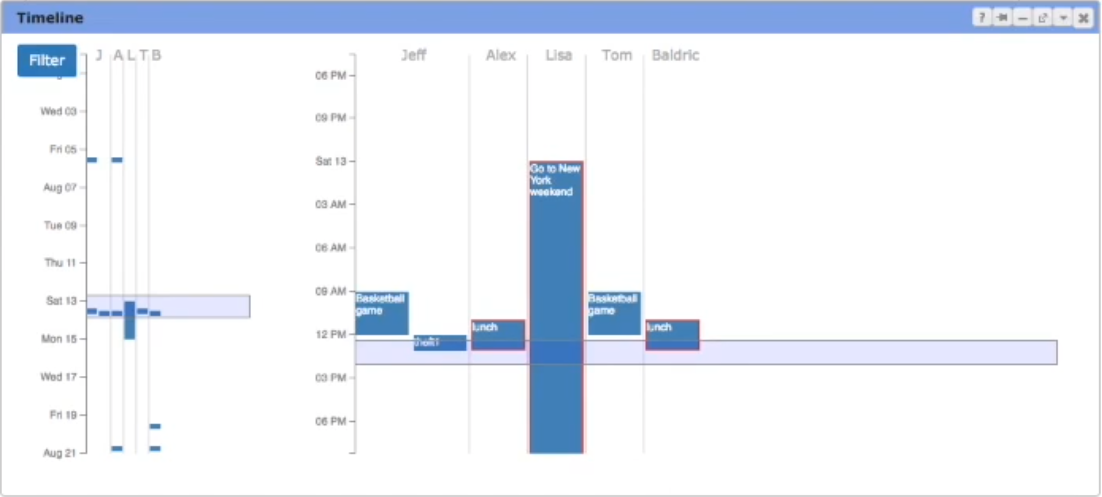
\includegraphics[width=\columnwidth]{03-System/img/timeline2.png}
	\caption{The improved timeline in CAnalytics V2 displays events schematized by people. Selection on the left overview panel zooms the view into a specific range of time. Selection on the right detailed view selects events that overlap with a time range and applies a filter to other views (e.g. map, table and network) to narrow down data relevant to the selected events. This tool helps find alibi of suspects and identify correlation of events/time with other pieces of information. \label{fig:timeline2}}
\end{figure}

\paragraph{Capability to restore deleted data}

In Study One we noticed that participants removed data that were not relevant to their hypothesis to reduce noise. For example, if they had excluded the possibility of a suspect, it made sense to remove the suspect from the visualizations. However, we found that it often happened that analysts refuted their hypotheses and rewound back to the original evidence. Going back and forth in the evidence is a frequent operation although analysts do not need all pieces of evidence all the time. 

In CAnalytics V2, instead of \emph{``deleting''} a data object, analysts can \emph{``archive'' } an object. Archived data are hidden in visualization such as the network and the map, but are still accessible in the data table. They were grayed out and ranked in the end, but were searchable and could be ``restored'' if needed. 

\paragraph{Animated change}

Another subtle improvement is adding animated change made by teammates. For example, when an analyst is deleting an object, collaborators can easily miss that person's intention to delete the object and even the deletion action itself. One design solution is to make small actions larger. In this case, we use animation to make the delete action more prominent. This could be done by adding a visual effect atop the deleted object to emphasize that it has been selected, and then adding an animation to the actual delete event to make it more salient, where it perhaps grows in size for a few seconds before shrinking to nothing \citep{Greenberg2001}. Similar animation is applied to adding a data object and editing an object.


\section{Use case demonstration}

To demonstrate the usage of the collaborative hypothesis development feature in CAnalytics V2, we run a use case in Table~\ref{tab:demo}. The full video is available at \url{https://youtu.be/pHqOukeg2KA}.

\begin{table}
	\caption{A demonstration of collaborative hypothesis development in CAnalytics V2}
	\label{tab:demo}
	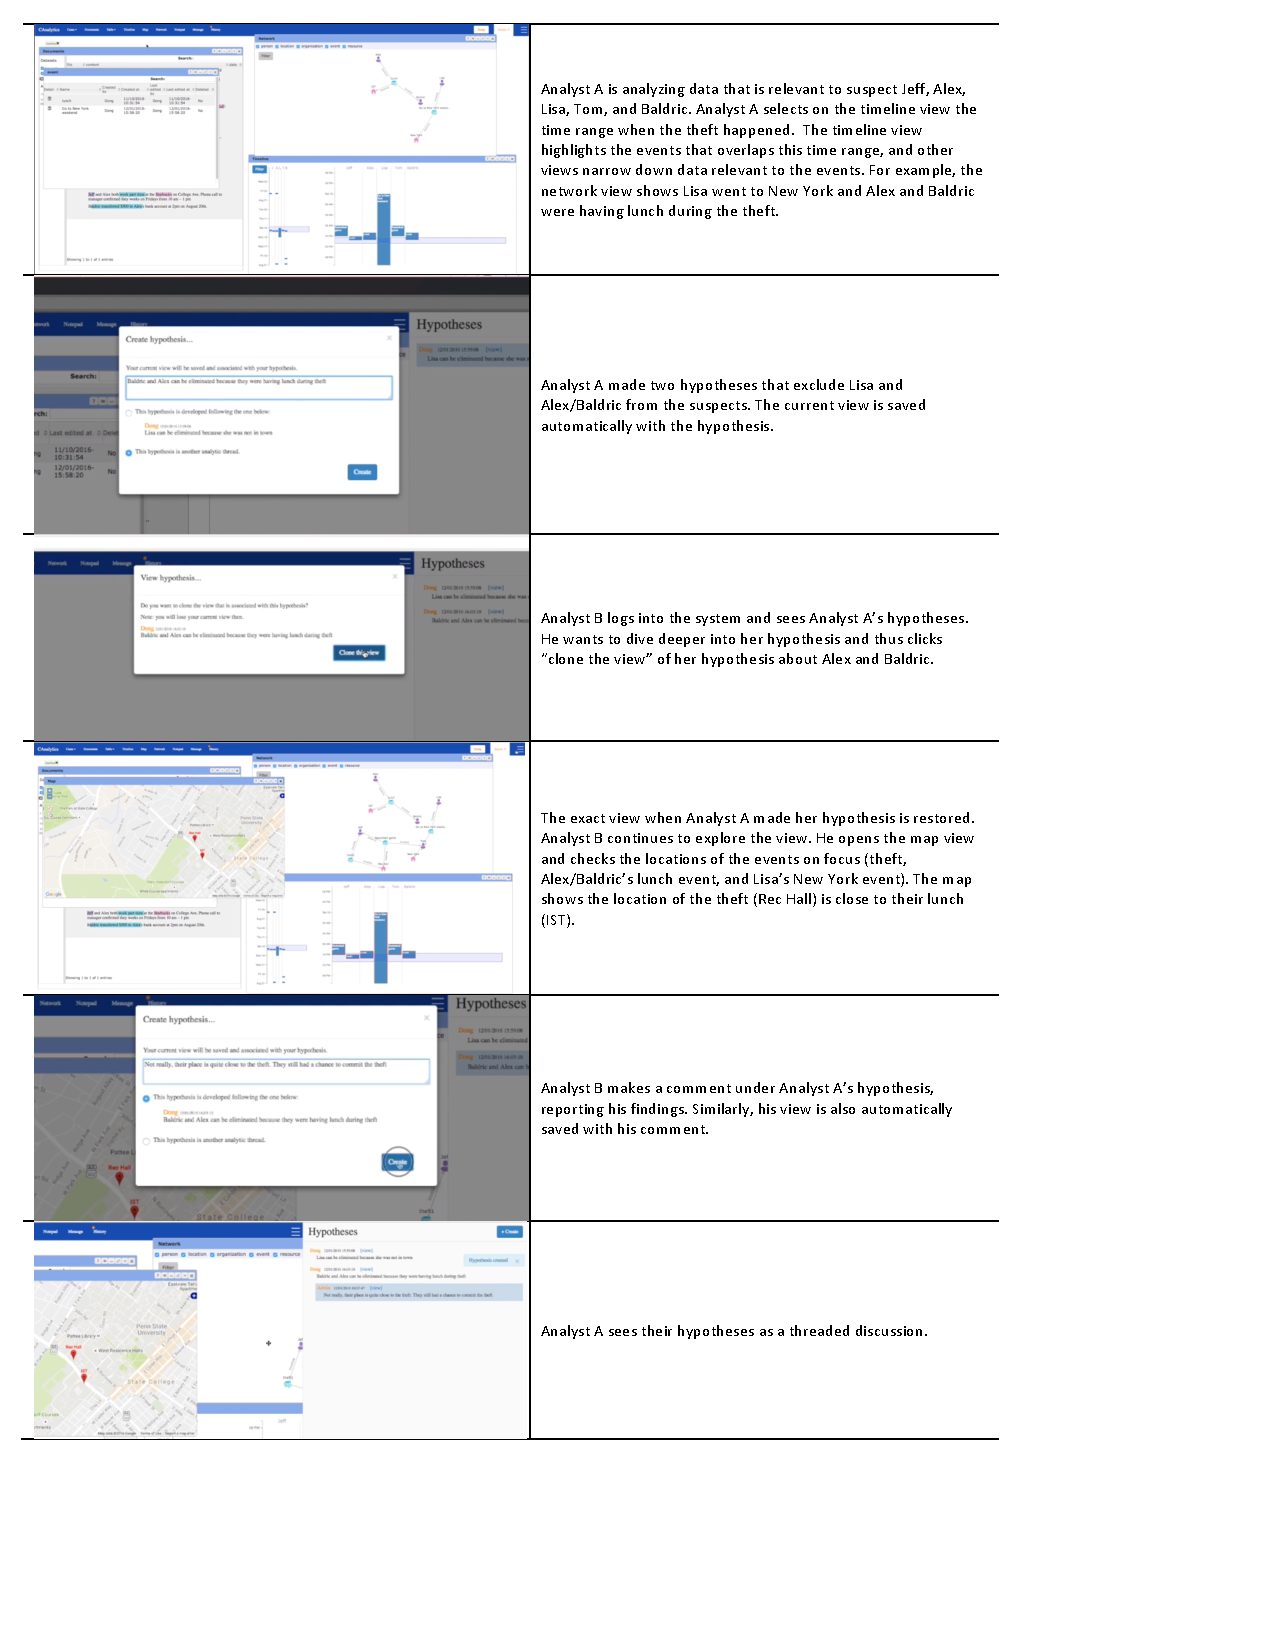
\includegraphics[width=1.2\columnwidth]{05-Study_two/img/demo.pdf}
\end{table}

\section{Classroom study setting}

 \begin{figure}
	\centering
	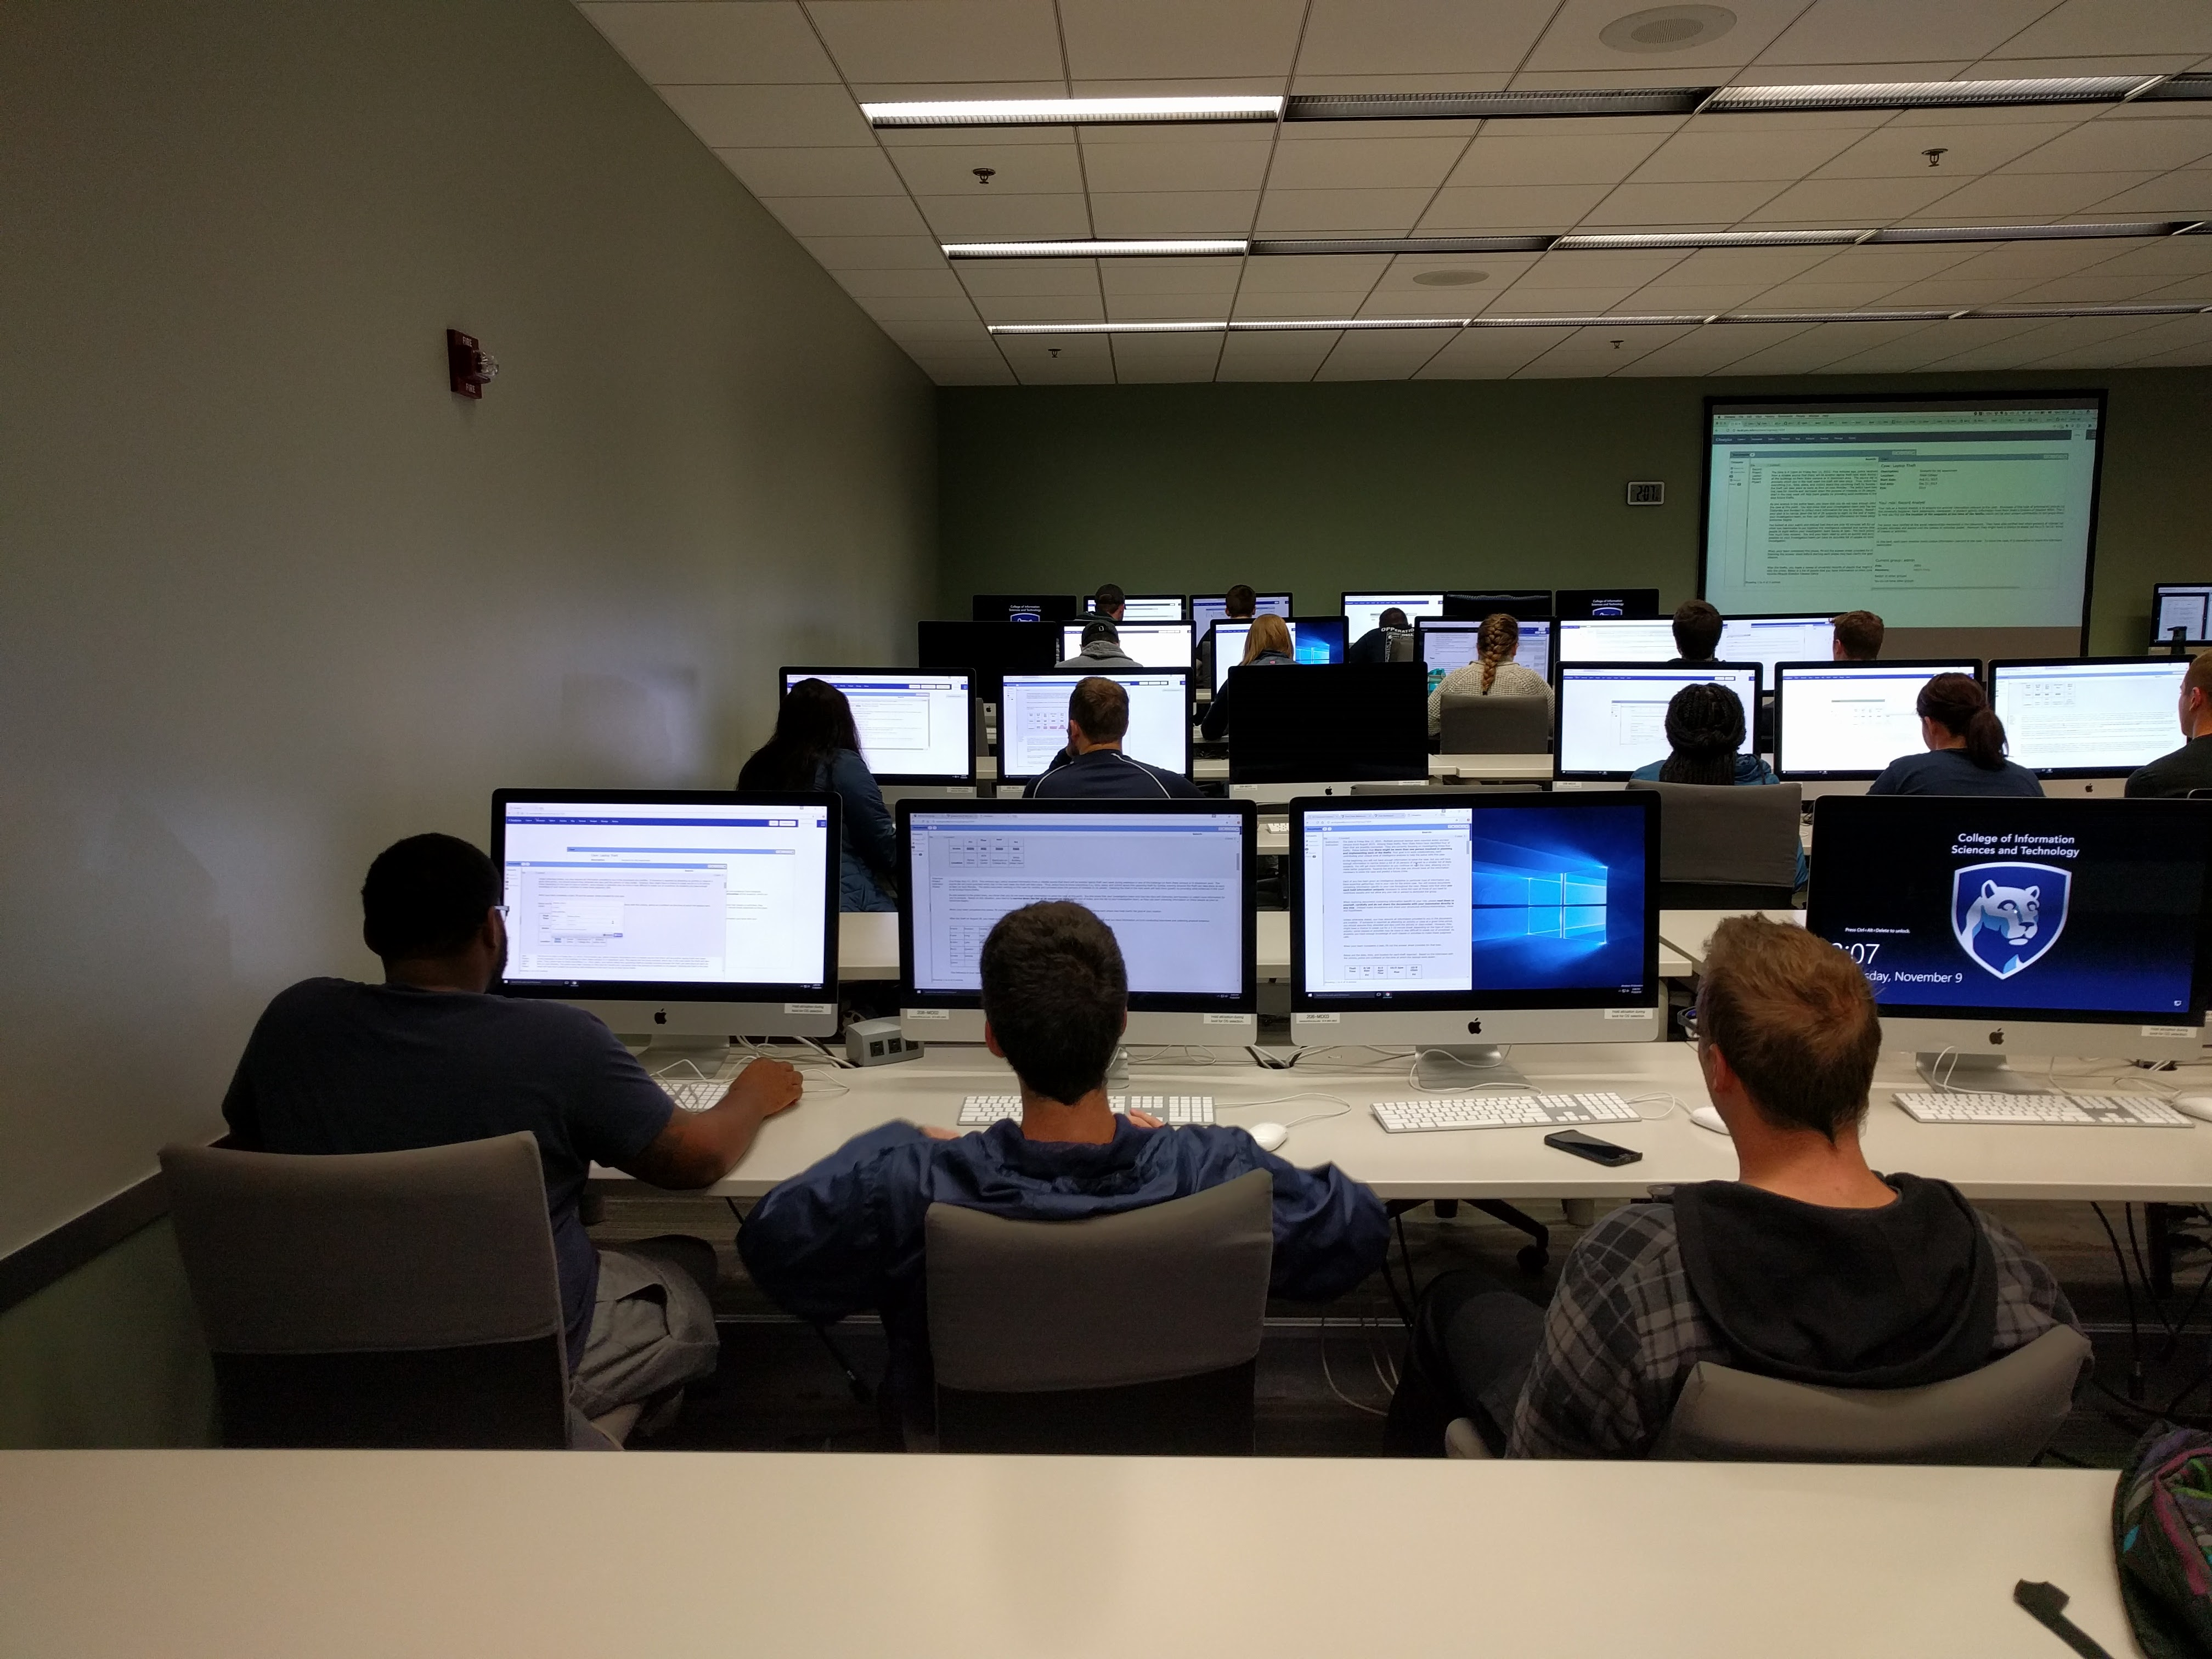
\includegraphics[width=.8\columnwidth]{05-Study_two/img/classroom_setting_2.jpg}
	\caption{The second classroom study setting}\label{fig:classroom2}
\end{figure}

We deployed CAnalytics in SRA 468, a course in the major of Security and Risk Analysis at Pennsylvania State University. The course was designed to teach senior undergraduate students about the application of visual analysis in the domain of intelligence analysis.

The study began in the later phase of the course, when students had learned about common techniques of visual analytics, such as time series analysis, tree-based data analysis, and network analysis, as well as popular visualization tools like ArcGIS and Tableau. With such equipment of basic visualization knowledge, from Nov 7 to Nov 18, we introduced CAnalytics and asked students to use the tool to solve a complex task.

Students were first given a tutorial and followed step-by-step instructions to use CAnalytics features to solve a simplified task. The students then had two full classes to do the project, each class lasting for 50 minutes. Due to the complexity of the task, students were asked to work for extra hours outside class.

The task used in the study was a fabricated laptop theft scenario. The task was applied and validated in earlier user studies \citep{Carroll2013, Borge2012}. The task consists of 222 pieces of information, involving social media data, bank transactions, suspect interviews, and other records. Teammates were randomly assigned one of the three roles and were responsible for a unique set of documents: a Web Analyst had social media data and would contribute mostly on social relationships; a Record Analyst had archival information about suspects' daily schedules and could contribute by providing locations of suspects when the theft occurred; and an Interview Analyst had interview data from people of interest and could contribute by identifying the motivation of suspects. To reach the right conclusion, teams had to share their unique information sufficiently. Students were told not to share documents directly but that they could share their information by creating data annotations in CAnalytics.

Of the 42 students enrolled in the course, 30 consented to our study and 21 (7 teams) finished the study (submitted reports for both phase 1 and phase 2 tasks). In our analysis, we focused on the 7 teams that completed both tasks. Of the 7 teams, one team (Team 163) in their post-task questionnaire reported that they ended up using Google Sheet to schematize data instead of CAnalytics. Therefore we excluded their interaction log in the analysis but kept their performance as a baseline reference for other teams.


\section{Data collection and analysis}

We did the same data collection as in the first classroom study. However, our analysis focuses on the part that relates to hypothesis development. In particular, we found user's answers to the open-ended survey questions most useful.  We asked participants to reflect the way how their team used the feature and how useful they thought of this feature. We triangulated their answer with their interaction logs captured by the system as well as hypotheses data saved in the system. This guarantees believable interpretation output in the study. In the result below, we describe our interpretations followed by users’ quoted comments. 
\section{Result}

\subsection{Confirming result from study one}

Many feedbacks from students in study two echo and confirm results from study one. For example, users like the feature that maps out annotated data objects to different visualizations. This allows them to put various perspectives into the otherwise unstructured text documents.

\begin{quote}
\emph{We feel that this service was helpful in that we could visually see the relationships that we mapped out as well as add our own parts to it without needing to email them to each other or having multiple networks.(P178)}
\end{quote}

Users also mentioned the usage of the new timeline. They appreciate the capability to match individual events against critical events; thus they can quickly target data of interest. The multiple tracks in the timeline view also encourage them to use the filter feature. 

\begin{quote}
\emph{It helped because we were able to see who was where at what times so when the crimes were taking place we knew who was near the crime or who was busy etc.(P150)}
\end{quote}

\begin{quote}
\emph{The main tool used to help eliminate subjects was by using the filter tool to see what suspects were not at the location of the thefts at the times for each incident (P188)}
\end{quote}

Users rate highly of the collaboration features. They feel the idea of sharing one common analytic artifact changes the way they collaborate. 

\begin{quote}
\emph{This differs because I can actually see what my team is doing as they are doing it, but we can also alter the information and that would change the entire network. Changing the network and altering information also updated and altered my own information, which was something new compared to the other tools I have used}
\end{quote}

One user also comments that he would first check his teammates' update before he sets out for his own analysis. 

\begin{quote}
\emph{Whenever I would work, I would go to the network first to see the connections that had been made. (P186)}
\end{quote}

Similar to the result in study one, students frequently associate CAnalytics with Google Docs and think of it as the Google Doc for analysts. 

\begin{quote}
\emph{CAnalytics tool is quite helpful when compared with other information analysis platforms such as google docs because it helps in real time annotating of various persons, relationships, events, etc. It also is a good tool when multiple people need to work on the same document and since it provides updates it helps reduce redundant work. Also, it provides additional features such as Timeline, Map, Network to help analyze information. (P193)}
\end{quote}

\begin{quote}
\emph{It gave us the ability to create and see the visuals that we would have only been writing about in programs like Google Docs. (P178)}
\end{quote}


\subsection{Feedback on hypothesis development tool}

Feedback on the structured approach for hypothesis development is mixed. We observe two major ways teams use this feature. First, they use it as a space for insight curation. As individuals go through annotation and visualization, they create notes about their hypotheses, findings, or ideas.

\begin{quote}
	\emph{The hypothesis was nice in the sense that it was a clean space to put final thoughts (p100)}
\end{quote} 

\begin{quote}
	\emph{As we went throughout our work we noted any important information and relationships that we found in the raw data to create hypotheses (P183)}
\end{quote}

These ideas then become a resource to which they refer when they compose their final report. This can be a useful feature as it helps analysts to focus on high level hypotheses instead of relooking at underlying data and visualizations. 

\begin{quote}
	\emph{I read through the hypothesis and used that to form my answers to the questions. (p183)}
\end{quote}


Secondly, participants use it to narrow down analysis and direct the team to focus on analyzing a particular aspect. When one team member creates a hypothesis, partners look into that hypothesis, retrieve the context where that hypothesis was generated, and help validate it connecting with their own knowledge. 

\begin{quote}
	\emph{It helped us focus and narrow in on an event and suspect.(P191)}
\end{quote}
\begin{quote}
	\emph{I confirmed the results by filtering out the maps, networks, and tables to confirm the conclusion. (P188)}
\end{quote}
\begin{quote}
	\emph{When my teammate shared a hypothesis about where some of the suspects work, I responded by using that hypothesis and applying it to my own analysis to see if I can make a connection between the hypothesis and the theft. (P198)}
\end{quote}


On the other hand, participants in one team commented that the way a hypothesis is generated does not follow their workflow. They reflect that when they find something interesting during their analysis, they would share it immediately with teammates (verbally). 

\begin{quote}
	\emph{We all agreed with each other when we posted hypotheses because we worked together the whole time (p100)}
\end{quote}

\begin{quote}
	\emph{We wrote it together so we didn’t really respond to it.(p150)}
\end{quote}

This team discusses possible hypotheses and comes up with a most reasonable one together. In other words, the team works closely in a synchronous manner to generate a hypothesis that everyone would agree on. This differs from the model our tool design was based on, which encourages frequent turn-around in developing a hypothesis; each turn-around would be more \textit{asynchronous} between which teammate would spend time assessing the validity of the last hypothesis. This closer approach to generating hypotheses seems prevalent as several teams mention the mismatch between the tool design and their workflow. This result is interesting as it is in contrast with the feedback on data annotation and visualization, for which the tool supports a similar structured technique. Participants mostly like those features as ``they reduced the efforts to frequently keep updated with the team''. We will extend exploration into this contrast in the discussion section.



One student mentions the scalability issue. When the team creates too many hypotheses, it becomes less efficient to continue developing these hypotheses. 

\begin{quote}
	\emph{we enjoyed making hypothesis together, and the tool quickly got out of hand when we all just tried tossing in info (P204)}
\end{quote}

It is true that the tool currently does not include any feature to search or manage hypotheses yet. The display is also not optimized for a large number of hypotheses. The goal of this study is to explore the feasibility of such a structured hypothesis development approach. But it will be an interesting future research topic to investigate how to enable large scale, long term hypothesis development and management. 

A few participants also mention the discoverability and usability issue of the feature. The feature is only accessible under a secondary menu in the system, thus it is not straightforward to start using the feature. The success of the tool also depends on how the whole team is using it. If one made a hypothesis but never got a response from the team, they gave up.

\begin{quote}
\emph{My team did not share a hypothesis, I created a couple but I did not get a response from my team (P186)}
\end{quote}

\begin{quote}
\emph{It was useful to see what they were indicating, but I still had to call them over to fully explain their rationale and logic. It was a good start point, but without them explaining in person to me what patterns they were seeing I was having difficulty making the same conclusions. (P204)}

\end{quote}

Interestingly, one participant did not use the feature but reflected that they probably should. 

\begin{quote}
\emph{We never completed a hypothesis within CAnalytics because it did not occur to us to do so. However, looking back, it might have been helpful to solve the case. (P197)}
\end{quote}

We do not know what makes him/her think that way, but research has observed such behavior before that might account for the reason. A structured technique demands more effort as users must explicitly externalize their thought, which takes more time than verbally communicating with teammates. Externalization, however, in the long run, benefits the team as they have an artifact for team reference. 




\section{Discussion}

The design goal of CAnalytics V2 is to support higher-level collaborative sensemaking while confirming the positive effect of integrating low-level data annotation and visualization efforts established in study one. Information analysis can be roughly divided into three key levels \citep{Pirolli2005,Kang2014a}: (1) identifying critical evidence; (2) organizing evidence into a schema; and (3) generating hypotheses based on evidence schema. Accordingly, CAnalytics provides data annotation, data visualization, and hypothesis threading tool for each level. Study one has suggested a positive impact with the integration of data annotation and visualization. Study two aims to provide a linkage between hypothesis development and data visualization and investigates the feasibility in a collaborative setting.

While collaboration occurred throughout the project, we observed that the degree of closeness in which they collaborated varied depending on the phase of analysis. When they set out the project, they usually had a close discussion on how they were going to tackle the problem strategically and how they would divide their work. This is often known as \emph{strategic coordination}, or functional collaboration \citep{Kang2011}. CAnalytics does not have a feature to explicitly support this, but we do observe participants discussing over the messaging tool. 

In our observation, teams then divided up the work and worked on their part individually. They still collaborated by sharing evidence they annotated, but the collaboration was looser because it was mostly \emph{content} sharing without a need for deep discussion. The real time sharing feature provided by CAnalytics helped facilitate collaboration. 

We observed a stronger demand for close collaboration in hypothesis development than in data annotation or visualization. We speculate that collaboration in higher level sensemaking requires a higher volume of information to be exchanged. While data annotation activities share only a piece of annotation, hypothesis development requires the sharing of a rich amount of evidence and schema at a high frequency. And based on the evidence, there can more than one direction analysts can draw from. The team needs a more synchronous, closer channel to exchange their ideas. This is probably why they would prefer to discuss over hypotheses together and compose hypothesis collectively.

This nuance in collaboration closeness suggests us to consider accounting for the different needs in our group design. Teammates in loosely coupled collaboration are weakly dependent on one another and can function autonomously, often without the need for immediate clarification or negotiation with others. Yet analysts in closely-coupled collaboration have high frequency of turn-arounds and high density information exchange, and thus a multi-channel communication is preferred. Groupware systems that are designed to support both couplings must address these differences. 



Another goal of this research is to explore alternatives to existing structured techniques such as Analysis of Competing Hypotheses (ACH). There are several key differences in our approach to hypothesis development.

First, it takes less effort to start generating a hypothesis. ACH asks analysts to cover a wide range of hypotheses in the very beginning; therefore it demands a decent level of experience and knowledge. It takes serious commitment to come up with all possible scenarios and often is intimidating enough to drive away junior analysts. In contrast, our approach is opportunistic. As analysts annotate key evidence in documents, they can create a hypothesis whenever they see a connection between two pieces of evidence. It makes analysts easier to get started and gain momentum to continue.

Second, the hypothesis development process is integrated with evidence annotation and analysis. Analysts can provide an associated visualization state for each hypothesis, and that visualization provides the full context with which partners can validate the hypothesis. Lacking context is often a critique of ACH \citep{Gelder2008} because each evidence/hypothesis is treated on its own. 

Third, hypotheses can be more flexibly structured. The matrix structure in ACH assumes hypotheses are isolated and are on a single level. It asks all hypotheses to be entered individually on the top row of the matrix. In reality, however, hypotheses can be more or less abstract or general. A hypothesis can have sub-hypotheses, and a hypothesis can be built upon another one. The threading structure in our approach allows for a more flexible way to develop hypotheses. A sub-thread can support, refute, or extend the parent thread. 

\section{Summary}
This chapter presents the second classroom study where senior undergraduate students were learning to apply visual analytic techniques on intelligence analysis and employed CAnalytics in their course project. With a focus on qualitative analysis on participants' answers, we confirmed results from the first study. Further, we identified different ways teams used the hypothesis development feature. While some teams used it as a collective insight curation space, other teams used it to direct the next collaboration opportunity. The result is followed by discussion on design consideration for nuance in collaboration closeness. In the next chapter, we will reflect on the two studies and discuss the lessons we learned overall.

\chapter{Discussion and Conclusion}
Design implications have been discussed at the end of each classroom study. This section discusses the reflection on my overall dissertation research.

\section{Design research}

Groupware research presents a lot of different challenges from research on individual tools. Groupware research involves dynamics between multiple individuals and such dynamics are heavily shaped and mediated by the tool. The tool and the team function as a single system in accomplishing a task. A single feature in the tool may change team behavior altogether. In single-user tool research, a research method that is often employed is to mock up features to test the user's reaction and mock out other features that researchers are not interested in. However, this method does not work for evaluating groupware. To understand how groupware will influence team dynamics, the groupware must be fully functional, with full capability to support team communication and coordination. The team dynamics cannot be simulated. 

Team dynamics take time to evolve. This includes the development of social awareness, situation awareness, workspace awareness, and activity awareness. Such awareness needs time to be established and maintained to a level where the team can start work effectively. This is also different from single-user research, in which user reaction to a tool can be mostly measured immediately. Longer-term research is preferred if we want to investigate the real impact of groupware. And again, to enable a longer-term investigation, full features of the groupware must be implemented. 

Teams behave totally differently with tools of different levels of collaboration support. Teams with the paper prototypes naturally do more synchronous, co-located collaboration than teams with computer prototypes supporting distributed work. To some extent, teams with the paper prototype are accomplishing a different \emph{task} than teams with computer support. 
Tasks people engage in or wish to engage in define requirements for artifacts. Those artifacts, in turn, open up new possibilities to accomplish the task, while, inevitably, introduce new errors and complexities in task performance. Again the new tasks devolve into requirements for further technology evolution, provoking another round of transaction. 

This cycle, known as task-artifact evolution (Figure~\ref{fig:task-artifact}) \citep{Carroll1992a}, drives the underlying rationale of my research on groupware: to develop a tool to drive task evolution in possible directions, understand the resulting team behavior, and in turn make design changes to the tool. The design, development, and evaluation iterations result in knowledge in team behavior and design implications for collaborative analytic tools, which eventually contribute to the exploration and understanding of the design space of groupware. 

I take a \emph{design research} approach \citep{Zimmerman2007a,Convertino2008e} to explore how interactive visualization could support collaboration. The goal of design research is to address the ``wicked problems'' \citep{Rittel1973} in real world and the increasing complexity of situations that need software support. The outcome of design research is not only artifacts of more effectiveness but also new knowledge that can inform future design. Therefore, the developed groupware is not only a team-supporting \emph{tool} that facilitates their intelligence analysis projects, but, and arguably more importantly, also a research \emph{instrument} that reveals team behaviors and patterns in that specific setting, and ultimately contribute to the knowledge pool of design rationale for groupware. 


\begin{figure}
	\centering
	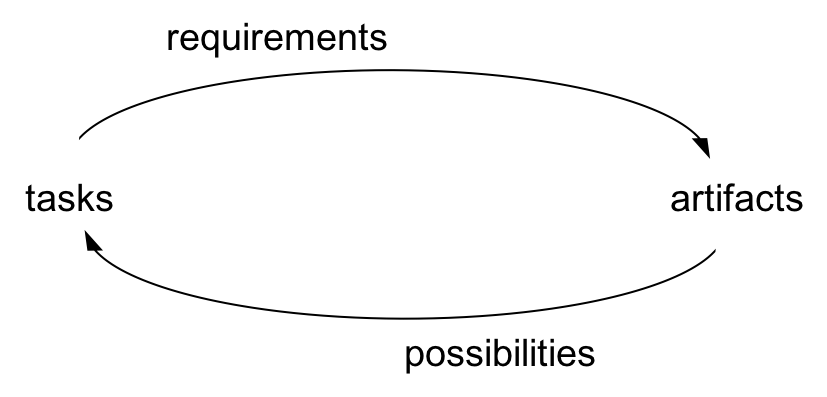
\includegraphics[width=\columnwidth]{06-Discussion/img/task-artifact-1.png}
	\caption{Task-artifact co-evolution structured with design methodology from \cite{Carroll1992a} \label{fig:task-artifact}}
\end{figure}


\section{Classroom study}

A critical requirement in design research is to understand the user's needs and practices. When these needs and practices are specialized, as is the case of Intelligence Analysis, it is 
particularly important to include the target user population in 
the design process. I take Intelligence Analysis as a specialized,
domain-specific task of information analysis. Therefore it is important to understand analysts with domain knowledge, 
learn their practice, and observe their reaction to tool features \citep{Scholtz2014}. 
However, professional analysts are hard to include 
in a long-term design cycle due to confidentiality and security 
issues. The classroom study provided an opportunity with deep 
access to analysts in training. These analysts have been trained 
with knowledge and skills of intelligence analysis, and have experience with state-of-the-art analytic
tools such as Analyst's Notebook and PARC ACH. In their reflections, participants often compared CAnalytics to
those tools, as well as the different teamwork experiences. Therefore, while their feedbacks are
admittedly not identical to experienced professionals,
they do provide a deeper insight into the strengths and
weaknesses of our tool than ordinary users. In addition, the students are young learners
that are willing to employ new work practices supported by features in
tools. They are important parts of the future intelligence community. In
this sense, their practice can be treated as a view into the future of
practice of the community \citep{Martin2014}.

Studies in this research spanned multiple user sessions.
This gave participants time to learn to adapt to team functions and to appropriate
the tool to best serve their team purpose. Teams were able to explore different team strategies and to
make changes if they got stuck \citep{Stahl2006}. For example, we
noticed that two teams decided to change the use of the tool halfway in
their analysis. One team started with dividing work by case documents
but later decided members should annotate different entity types.
Another team started with an accretion strategy by annotating all
entities and later discovered that this strategy brought too much
noise and decided to clean out irrelevant entities (filtering
strategy). Such change occurs as a consequence of increased awareness of
team functions and tool capabilities, which takes time to develop.

With deep access to these analysts, I can interpret and triangulate our data from multiple sources. I qualitatively analyzed participants' feedback to understand their first-person experience and corroborated them with surveys and interaction logs. The interaction logs provided us a detailed view of their analysis process and allowed us to quantitatively characterize their team behavior. Finally, their analytic products, including the visual artifacts and team reports, helped us distinguish team outcomes. In summary, this research contributes to the study of computer-supported collaboration work with valuable empirical data.

Yet classroom study also has limits. For example, many factors and
variables could exist that affect team performance. The fact that these
factors are often impossible to model or control adds to the difficulty
in data analysis (e.g.~teammate absence). Also, data collection is
challenging because team interactions are not always accessible. Teams
can choose to work synchronously or asynchronously, and it is difficult
to predict when or where the interaction of most interest is to occur.
Verbal communication is not accessible, which could be useful to infer
team awareness as a complement to interaction logs. Our work identifies
both positive evidence and problematic situations, and propose potential
solutions and possible hypotheses, yet rigorously evaluating these
solutions and validating hypotheses is beyond this study. Lab studies
and case studies can be conducted in the future to address these
problems with greater control and deeper data access.

\section{Analyst in control}

Throughout our study we observed that analysts are constantly annotating new data, restructuring existing annotations, archiving irrelevant data, and examining data in visualization. This is an extension compared to many other visualization tools, with which users are faced with pre-populated data and tasked with creating visual mappings to identify hidden patterns behind the data. In Intelligence Analysis and many other information analysis tasks, analysts frequently create and re-recreate data models to serve their analysis as their hypothesis evolves.

Data modeling is often seen as a precondition to perform any visual analysis. Data modeling transforms raw data to structured entities that are readable and processable to software. The focus of Visual Analytics has been largely put on combining automated modeling with interactive visualizations to facilitate reasoning \citep{Keim2010}, emphasizing the role of human in the loop of visualization and insight generation. In practice, however, we find that data modeling is an iterative process that is intermingled with visual analysis. New insights inspires analysts to re-model data either in a different scope (horizontally) or in a different level of detail (vertically). 

Horizontally, analysts annotate different parts of the data. For example, an intelligence project typically includes data that consists of a series of \textit{critical events}. Analysis of the data though can focus on some of the events. Analysts decide which events to look into first. As they come up with new hypotheses or need more data to validate his hypothesis, they may continue annotating and visualizing other events.

Vertically, analysts annotate data to the level of detail they prefer at the moment of their analysis. The same piece of a document can be annotated in different ways according to the analyst's need. For example, when the analysts are in the early phase of the investigation and want to get an overview of all events, they can annotate an event with time, place, and a brief summary. As they get more interested in a specific event, they can add the people that were involved and tools/resources that were used in the event. If the event becomes critical and needs to be compared with other events to find patterns, analysts might annotate the step-by-step process how people did it in the event. In contrast, if an event becomes irrelevant to the hypothesis, the analysts may remove its details or the event altogether to avoid distraction. 

We use annotation to allow analysts to create and modify their data of interest. This complements the popular approach which employs 
automated modeling such as natural language processing (NLP) techniques to extract and
model entities \citep{Bier2010, Stasko2008}. While algorithms for named
entity recognition have improved significantly, developers of the
entity-based systems \citep{Gorg2014} admitted that the
accuracy of automatic entity extraction is not sufficient to support
human analysis. This is especially true when the tasks are exploratory in nature, where the questions are ill-defined and no training data is available \citep{thomas2005illuminating}. Besides, relationships identified by algorithms are
limited to the co-occurrence of entities in the same document, whereas
identifying meaningful relationships \emph{implicit} in documents that
are of more importance to analysts is not possible. And perhaps the most
problematic is the fact that the NLP treats all pieces of information
equally with no regard to the problem analysts have at hand. 

We posit
that information analysis is a progressive process, wherein analysts
place a varying priority on evidence depending on how they frame the
problem \citep{Heuer1999}. Annotation allows for user
control in the process, allows integrated source data objects to be identified,
and avoids the problems associated with automatic identification of
disaggregated people, locations, and times \citep{Bier2008}. Analysts can
decide their own information of interest and granularity that best suits
their ad-hoc analytic needs. The guide to visually exploring data ``Overview first, zoom and filter, then details-on-demand'', as proposed by \cite{shneiderman2003eyes} describes how data should be presented on screen. We suggest extending the guide to be ``Overview first, model data, analyze, zoom and filter, re-model, then details on demand''.

\section{Collaboration, structured technique, and the role of computing tools}

Collaboration is, in essence, the development of \textit{content} common ground and \textit{process} common ground within a team \citep{Convertino2009}. Content common ground encompasses ``I know that you know that I know \textit{what}''. It is the result of information sharing. Process common ground encompasses ``I know that you know that I know \textit{how}''. This is the shared understanding across team members of the procedures, rules, and manner in which collaboration will occur. Process common ground helps teams achieve high awareness and result in content common ground.

Process common ground can be achieved with ad-hoc team discussion and negotiation, or agreement on a predefined set of procedures. Structured technique is such a predefined set of procedures, rules, and manner in information analysis. Structured technique breaks down information analysis into a defined process of reasoning, and define a set of procedures teammates agree upon \textit{before} they start to collaborate on work. With all analysts understanding the structured technique, it provides teams with a base process common ground. Following the structured techniques, each team member has their role and task. By implementing the technique, individuals focus on their own piece of work, while understanding what and why teammates are working on, without constantly re-coordinating and re-aligning team intentions and individual behaviors. Structured technique has little dependency on the team attributes or individual experience, and thus can be applied to various teams with relative ease. In that sense, It is a methodology of common ground development that can be abstracted and generalized to collaboration between other teams, to enable effective teamwork. 

Structured technique emphasizes the externalization of reasoning and preserve the process that leads to the conclusion. Human mind is often blamed for its stateless memory--people keep updated with the current thinking, but lose track of the last idea even seconds ago. Information analysis typically takes an extended period of time, and the final conclusion may differ completely from the original hypothesis. The situation becomes even worse in collaborative work. People fail to recall arguments or evidence from teammates. Structured techniques help organize information in a structured manner. For example, our tool requires analysts to put facts and relationships in a structured form. These representations can easily be shared across teammates. With real time sharing, every creation or modification of externalization is streamed to teammates as partner's action along the course, contributing to the development of team awareness. Structured technique preserves the path of reasoning, including the proposal of a hypothesis, evidence favoring or against the hypothesis, and development of the hypothesis. Such information provides references to team collaboration, anchors over which teams can discuss and improve.

Structured techniques are yet tedious to implement manually. It requires a lot of effort to externalize information and keep it organized. This is where computing tools come in. Computers are efficient at keeping consistent data structures and make cross-referencing data entities straightforward. There are at least four functions computing tools can support: 1) Keeping data input consistent from collaborators. Individuals from different backgrounds and roles could have different input habits and formats. The tool can enforce a format that complies with the structured technique. 2) Visualize information. 3) Share information and team actions properly. 4) Identify opportunities for collaboration.

\begin{figure}
	\centering
	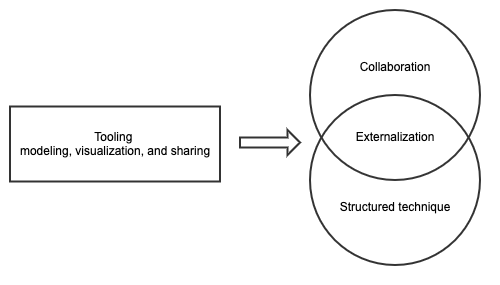
\includegraphics[width=\columnwidth]{06-Discussion/img/theory.png}
	\caption{Structured techniques, collaboration, and tooling}
\end{figure}


\section{Education in collaborative information analysis}

An important direction of this research is to explore how such a collaborative instrument could be employed to support collaborative learning in education. We studied an introductory intelligence analysis course, but many other courses involve heavy information analysis tasks, in which snippets of information must be annotated and analyzed with respect to concepts, connections, weights of evidence, and pros and cons of opinions. This is similar to generating and evaluating hypotheses in our case. Thus one could imagine courses in business, new media, and those involving heavy literature review adopting this tool similar to the case described here.

The goal is to shape students' behavior towards more collaborative learning. With traditional single-user tools, students often employ a divide-and-conquer strategy; they divide their job responsibility, work individually on their own part, and put the results together in the end for report submission. In our study, we observed that students spontaneously conducted closer collaboration and enjoyed being able to contribute simultaneously.
% cite education paper in intelligence analysis

In addition to shaping the \textit{learning} behavior of students, a collaborative supporting tool can also change how an instructor \textit{teaches} analytic skills. Anecdotal reflections from the instructor in our classroom study emphasized the role of system support in \textit{instructor intervention}. During our classroom study, the instructor frequently went over to the student's desk and checked how they were doing. The instructor commented that he valued students' analytic process as much as their final report. His emphasis on analytic process is consistent with the value of the intelligence community, who claimed that analysts \textit{``should think about how they make judgments and reach conclusions, not just about the judgments and conclusions themselves''} \citep{Heuer1999}. However, the process is hard or costly to capture for assessment in reality. In the context of education, for example, all students are conducting analysis at the same time. Without explicit support, the instructor has limited supervision over the process.

The collaborative learning instrument is likely to provide an opportunity to get a student's analytic traces preserved and assessed because the system has already captured and saved user interactions. These logs are currently saved for research purposes in our study, but potentially they can be displayed to the instructor for assessment purposes. Taking advantage of the system's synchronization capability, student's behavior can be streamed to a ``monitoring dashboard'' in real time, from which the instructor could check student's progress and take early intervention if any team deviates from the expected path.

\section{Summary}

This dissertation contributes an understanding of how analysts use groupware to analyze complex datasets over extended periods. The research presents a design process that identifies design requirements from task analysis, embodies requirements into groupware prototypes, observes team behavior mediated by the tool, and then repeats the process. Through a series of user studies, I investigated how we can better support collaborative information analysis. To this end, I implemented and evaluated two versions of a groupware tool to understand the effects of these design considerations on collaboration. Here is a brief review of the major contributions of the dissertation.

\textbf{C1: A characterization of collaborative information analysis activities.} 
These activities include data modeling, visual analysis, and hypothesis development. Structured techniques such as ACH and link analysis are often employed in the process. Collaboration is often impeded by the limit of concurrency and manual sharing.

\textbf{C2: A fully functional tool that supports collaborative information analysis.}
Features of the tool include integrated support for data modeling, visual analysis, and hypothesis development, a structured approach for data analysis activities, team awareness support, and capture of high-level, semantic usage logs. The architectural design and implementation can help future groupware overcome technical issues in synchronicity enablement and complex state management.

\textbf{C3: A characterization of analysts' team behavior mediated by groupware over extended periods.}
Evaluation of the tool through two classroom studies with analysts-in-training reveals various team behaviors such as filtering and accretion, situational logic and comparison, inferential connection and factual discrete, as well as a loose coupling in data modeling and close collaboration in hypothesis development. The result highlights the importance of providing an integrated workspace that supports the smooth transition of analytic activities.

\textbf{C4: Design guidelines to improve collaborative information analysis support.}
These guidelines include properly representing uncertainty both from data and from teammates, building collapsible views for hierarchical data, treating views as a team resource like data that are sharable, extensible, and reusable, distinguish visible and valuable contributions to encourage high-quality participation, and supporting multiple levels of collaboration closeness throughout the analysis lifecycle. It also calls for a combination of structured technique and awareness technology to better support collaborative information analysis.





%% now we include the appendices
%\appendices
%\chapter{Team analysis report template}
%

% 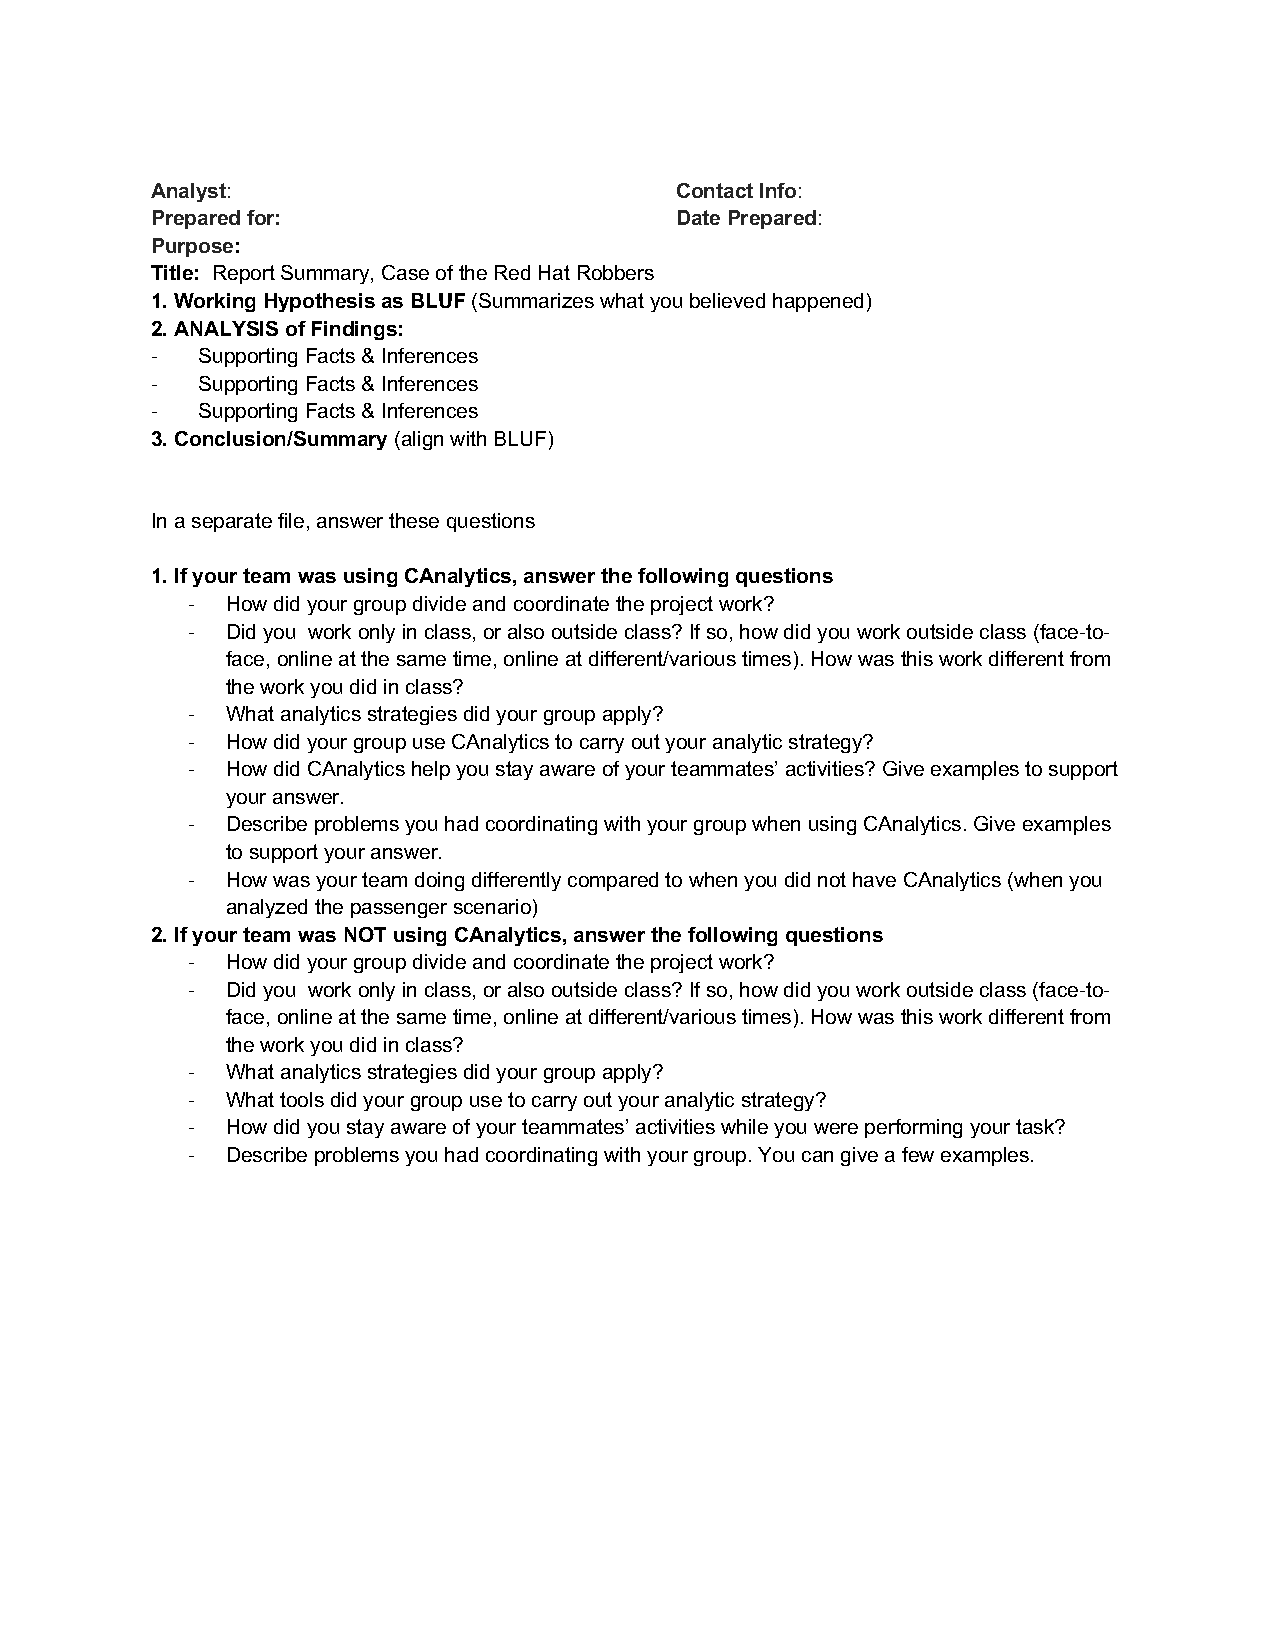
\includepdf[pages=-]{appendix/analyst_report.pdf}
%% omit this if there are no appendices

%% if there is only one appendix,
%% say \singleappendix instead of \appendices
% \singleappendix

%% these are the actual commands to include the apendix files:



%\include{ap-more}


%% finally comes the bibliography and vita
%% the bibliography is generated automatically using BibTeX
%% Note: in order to get the (author year) citation style, this example
%% includes a different *.bst style file than psuthesis.bst.  Sarah found
%% this style file on: http://www.ee.oulu.fi/~harza/latex/
%% This style includes the paper titles in the bibliography, so use it
%% if you want:
%\bibliographystyle{/enter/path/to/ayphdthesis_mod}
%% However, according to the grad school thesis guide (c.2004), there is no
%% special formating required for the bibliography, and to just follow
%% the citation styles of your field, in that case the ``apj'' style is
%% prefectly OK, so that is the one that is going to be included in this
%% example file (use whichever style you prefer):
\bibliographystyle{plainnat}

%% the following is the path to you *.bib file
%% (you do not need to enter the ``.bib'' extention)
\bibliography{./Dissertation}

%% ADS can generate the entries in the bib file for you, just call up
%% the abstract, then near the bottom of the abstract page there is a
%% link to ``Bibtex entry for this abstract'' - just copy that into
%% your bib file.  Here is an example bibtex entry:
%% @ARTICLE{citecode,
%%    author = {{Smith}, J. and {Jones}, M.},
%%     title = "{This Paper has some Really Cool Results}",
%%   journal = {\aj},
%%      year = 2002,
%%     month = sep,
%%    volume = 123,
%%     pages = {1-20},
%%    adsurl = {http://adsabs.harvard.edu/cgi-bin/nph-bib_query?bibcode=2002AJ....123.1S&amp;db_key=AST},
%%   adsnote = {Provided by the NASA Astrophysics Data System}
%% }
%% NOTE: ADS returns the AASTeX code for the journal name, you'll either
%% have to change that by hand in each bib entry, or include a
%% definition of the codes in your ``definitions'' file so LaTeX doesn't
%% freak out.  Also, what I entered as ``citecode'' can be changed to
%% whatever you want to use in the citations in the document, i.e., for
%% ``\citet{citecode}'' or ``\citep{citecode}''.

%
%%% the thesis must end with a Curriculum Vitae (**one page or less**)
%%% (this is Sarah's formatting, not sure how it compares to the other examples)
%\vita
%\Large
%\vspace*{-0.4truein}
%\centerline{{\bf Your Name Here}}
%
%\medskip
%
%\large
%\centerline{{\bf Education}}
%\normalsize
%
%\smallskip
%
%\par\noindent
%%\textbf{\{The Pennsylvania State University}}\, State College, Pennsylvania\hfill 199?--Present
%
%\smallskip
%
%\par\noindent
%\hspace{0.10truein}
%\parbox{6.15truein}{
%\par\noindent
%Ph.D. in Astronomy \& Astrophysics, expected in (Month) (Year) \\ Area
%of Specialization: Something }
%
%\medskip
%
%\par\noindent
%\textbf{\textit{(Undergrad Institute Name)}}\, (City), (State)\hfill 199?--199?
%
%\smallskip
%
%\par\noindent
%\hspace{0.10truein}
%\parbox{6.15truein}{
%\par\noindent
%B.S. in Physics (or whatever), \textit{cum laude} with distinction in the major (etc.)
%}
%
%\medskip
%
%\large
%\centerline{{\bf Awards and Honors}}
%\normalsize
%
%\smallskip
%
%\par\noindent
%Award Name \hfill year\\
%Another Award \hfill 200?--200?\\
%One more for good measure \hfill 200?, 200?
%%NASA Graduate Student Research Program Fellowship\hfill2000--Present\\
%%Pennsylvania Space Grant Consortium Fellowship\hfill1998--2000, 2000--Present\\
%%Zaccheus Daniel Foundation for Astronomical Science Grant\hfill1999, 2000\\
%%University Graduate Fellowship\hfill1997--1998\\
%%Roberts Fellowship, Eberly College of Science\hfill1997--1998\\
%%Summer Study Grant, Holderness School\hfill1996
%
%\medskip
%
%\large
%\centerline{{\bf Research Experience}}
%\normalsize
%
%\smallskip
%
%\par\noindent
%\textbf{\textit{Doctoral Research}}\, The Pennsylvania State University\hfill199?--Present
%\par\noindent
%Thesis Advisor: Prof. Someone R. Other
%
%\smallskip
%
%\par\noindent
%\hspace{0.10truein}
%\parbox{5.7truein}{
%\par\noindent
%This research involved lots of cool stuff.
%}
%
%\medskip
%
%\par\noindent
%\textbf{\textit{Graduate Research}}\, The Pennsylvania State University\hfill 199?--199?
%\par\noindent
%Research Advisor: Prof. Someoneelse R. Other
%
%\smallskip
%
%\par\noindent
%\hspace{0.10truein}
%\parbox{5.7truein}{
%\par\noindent
%This research also involved lots of cool stuff.
%}
%
%\medskip
%
%\par\noindent
%\textbf{\textit{Undergraduate Research}}\, Undergrad University\hfill 199?--199?
%\par\noindent
%Research Advisor: Prof. Name Goes Here
%
%\smallskip
%
%\par\noindent
%\hspace{0.10truein}
%\parbox{5.7truein}{
%\par\noindent
%Really cool stuff is what I did for this research.
%}
%
%\medskip
%
%\large
%\centerline{{\bf Teaching Experience}}
%\normalsize
%
%\smallskip
%
%\par\noindent
%\textbf{\textit{Guest Lecturer}}\, The Pennsylvania State University\hfill 199?--Present
%
%\smallskip
%
%\par\noindent
%\hspace{0.10truein}
%\parbox{5.7truein}{
%\par\noindent
%I taught lectures which involved doing cool stuff.
%}
%
%\medskip
%
%\par\noindent
%\textbf{\textit{Teaching Assistant}}\, The Pennsylvania State University\hfill 199?
%
%\smallskip
%
%\par\noindent
%\hspace{0.10truein}
%\parbox{5.7truein}{
%\par\noindent
%I taught labs and did cool stuff.
%}
%
%\medskip
%
%\par\noindent
%\textbf{\textit{Another Experience}}\, Some School, Some City, Some State\hfill 199?--199?
%
%\smallskip
%
%\par\noindent
%\hspace{0.10truein}
%\parbox{5.7truein}{
%\par\noindent
%I taught cool stuff to cool people.
%}

% \end{singlespace}
\end{document}

%%% Local Variables:
%%% mode: latex
%%% TeX-master: t
%%% End:
